%----------------------------------------------------------------------------------------
%	PACKAGES AND OTHER DOCUMENT CONFIGURATIONS
%----------------------------------------------------------------------------------------

\documentclass[
11pt, % The default document font size, options: 10pt, 11pt, 12pt
%oneside,% Two side (alternating margins) for binding by default, uncomment to switch to one side
twoside,
english, % ngerman for German
singlespacing, % Single line spacing, alternatives: onehalfspacing or doublespacing
%draft, % Uncomment to enable draft mode (no pictures, no links, overfull hboxes indicated)
%nolistspacing, % If the document is onehalfspacing or doublespacing, uncomment this to set spacing in lists to single
%liststotoc, % Uncomment to add the list of figures/tables/etc to the table of contents
%toctotoc, % Uncomment to add the main table of contents to the table of contents
%parskip, % Uncomment to add space between paragraphs
%nohyperref, % Uncomment to not load the hyperref package
headsepline, % Uncomment to get a line under the header
%chapterinoneline, % Uncomment to place the chapter title next to the number on one line
%consistentlayout, % Uncomment to change the layout of the declaration, abstract and acknowledgements pages to match the default layout
]{MastersDoctoralThesis} % The class file specifying the document structure

\usepackage[utf8]{inputenc} % Required for inputting international characters
\usepackage[T1]{fontenc} % Output font encoding for international characters

%\usepackage{mathpazo} % Use the Palatino font by default

\usepackage[backend=bibtex,style=numeric,natbib=true]{biblatex} % Use the bibtex backend with the authoryear citation style (which resembles APA)

\addbibresource{../config/references.bib} % The filename of the bibliography

\usepackage{tikz}
\usepackage{pgfplots}
\pgfplotsset{compat=1.7}

\usetikzlibrary{arrows,calc,shapes,decorations.pathreplacing,calligraphy}
\tikzset{>=latex}
	

	%% --------- Nodes ----------- %%
	
\tikzstyle{tensor}=[rectangle,draw=blue!50,fill=blue!20,thick,minimum height=0.55cm,minimum width=0.55cm]

\tikzstyle{matrix}=[diamond,draw=blue!50,fill=blue!20,thick,minimum height=0.5cm,minimum width=0.5cm]

\tikzstyle{operator}=[circle,draw=gray!80,fill=gray!50,thick,minimum height=0.6cm]

\tikzstyle{twositeop}=[draw=gray!80,fill=gray!50,thick,minimum height=0.6cm,rounded corners=0.3cm]
 
\tikzstyle{tensorl}=[rectangle,draw=orange!90,fill=orange!60,thick,minimum height=1cm,minimum width=0.6cm,rounded corners=0.1cm]

\tikzstyle{tensorc}=[rectangle,draw=red!90,fill=red!60,thick,minimum height=1cm,minimum width=0.6cm,rounded corners=0.1cm]

\tikzstyle{tensorr}=[rectangle,draw=violet!90,fill=violet!60,thick,minimum height=1cm,minimum width=0.6cm,rounded corners=0.1cm]



	%% --------- Custom Shapes ---------%%

\newcommand{\Left}[3]{
 	\pgfmathparse{#1 + #3}
 	\node[tensor] (tens) at (#1 , #2) {};
	\node (d1) at (\pgfmathresult , #2 + 1.5) {};
 	\node (d2) at (\pgfmathresult , #2 - 1.5) {};
 	\node (d3) at (\pgfmathresult , #2) {};    
    
    \draw[-] (d1.west) .. controls (#1, #2 + 1.5) .. (tens.north);
    \draw[-] (d2.west) .. controls (#1, #2 - 1.5) .. (tens.south);
	\draw[-] (tens) -- (d3);
}

\newcommand{\Right}[3]{
 	\pgfmathparse{#1 - #3}
 	\node[tensor] (tens) at (#1 , #2) {};
	\node (d1) at (\pgfmathresult , #2 + 1.5) {};
 	\node (d2) at (\pgfmathresult , #2 - 1.5) {};
 	\node (d3) at (\pgfmathresult , #2) {};    
    
    \draw[-] (d1.east) .. controls (#1, #2 + 1.5) .. (tens.north);
    \draw[-] (d2.east) .. controls (#1, #2 - 1.5) .. (tens.south);
	\draw[-] (tens) -- (d3);
}

\newcommand{\SVD}[3]{
 	\node[tensor] (U) at (#1 , #2) {};
	\node (Ulabel) at (#1 , #2 + 0.6) {$U$};
	\draw[-] (U) -- (#1 -0.8, #2);
	\draw[-] (U) -- (#1 , #2 - 0.8); 	
 	
 	\node[matrix] (S) at (#1 + #3, #2) {};
 	\node (Slabel) at (#1 + #3 , #2 + 0.6) {$S$};	
 	
 	\node[tensor] (V) at (#1 + #3 *2 , #2) {};
 	\node (Vlabel) at (#1 + #3 *2 , #2 + 0.6) {$V^{\dag}$};
 	\draw[-] (V) -- (#1 + #3 *2 +0.8, #2);
	\draw[-] (V) -- (#1 + #3 *2 , #2 - 0.8);
	
	\draw[-] (U) -- (S);
	\draw[-] (V) -- (S);
}

\newcommand{\Lfix}[4]{
 	\pgfmathparse{#1 + #3}
 	\node[matrix] (tens) at (#1 , #2) {$\boldsymbol{l}$};
	\node (d1) at (\pgfmathresult , #2 + #4) {};
 	\node (d2) at (\pgfmathresult , #2 - #4) {};    
    
    \draw[-] (d1.west) .. controls (#1 + 0.5 * #3, #2 + 0.5 * #4) .. (tens.north);
    \draw[-] (d2.west) .. controls (#1 + 0.5 * #3, #2 - 0.5 * #4) .. (tens.south);
}

\newcommand{\Rfix}[4]{
 	\pgfmathparse{#1 - #3}
 	\node[matrix] (tens) at (#1 , #2) {$\boldsymbol{r}$};
	\node (d1) at (\pgfmathresult , #2 + #4) {};
 	\node (d2) at (\pgfmathresult , #2 - #4) {};
    
    \draw[-] (d1.east) .. controls (#1 - 0.5 * #3, #2 + 0.5 * #4) .. (tens.north);
    \draw[-] (d2.east) .. controls (#1 - 0.5 * #3, #2 - 0.5 * #4) .. (tens.south);
} % Additional preambles

\usepackage[autostyle=true]{csquotes} % Required to generate language-dependent quotes in the bibliography

%----------------------------------------------------------------------------------------
%	MARGIN SETTINGS
%----------------------------------------------------------------------------------------

\geometry{
	paper=a4paper, % Change to letterpaper for US letter
	inner=2.5cm, % Inner margin
	outer=2.6cm, % Outer margin
	bindingoffset=.7cm, % Binding offset
	top=1.5cm, % Top margin
	bottom=1.5cm, % Bottom margin
	%showframe, % Uncomment to show how the type block is set on the page
}


%----------------------------------------------------------------------------------------
%	THESIS INFORMATION
%----------------------------------------------------------------------------------------

\thesistitle{Gradient-Based Optimal Control of Quantum Many-Body
Systems in Optical Lattices} % Your thesis title, this is used in the title and abstract, print it elsewhere with \ttitle
\supervisor{Jakob F. Sherson} % Your supervisor's name, this is used in the title page, print it elsewhere with \supname
\examiner{} % Your examiner's name, this is not currently used anywhere in the template, print it elsewhere with \examname
\degree{Masters Degree} % Your degree name, this is used in the title page and abstract, print it elsewhere with \degreename
\author{Frederik S. M\o ller \\ 201303717} % Your name, this is used in the title page and abstract, print it elsewhere with \authorname
\addresses{} % Your address, this is not currently used anywhere in the template, print it elsewhere with \addressname

\subject{Physics} % Your subject area, this is not currently used anywhere in the template, print it elsewhere with \subjectname
\keywords{} % Keywords for your thesis, this is not currently used anywhere in the template, print it elsewhere with \keywordnames
\university{Aarhus University} % Your university's name and URL, this is used in the title page and abstract, print it elsewhere with \univname
\department{Department of Physics and Astronomy} % Your department's name and URL, this is used in the title page and abstract, print it elsewhere with \deptname
\group{Quantum Measurement and Manipulation Group} % Your research group's name and URL, this is used in the title page, print it elsewhere with \groupname
\faculty{Science and Technology} % Your faculty's name and URL, this is used in the title page and abstract, print it elsewhere with \facname

\AtBeginDocument{
\hypersetup{pdftitle=\ttitle} % Set the PDF's title to your title
\hypersetup{pdfauthor=\authorname} % Set the PDF's author to your name
\hypersetup{pdfkeywords=\keywordnames} % Set the PDF's keywords to your keywords
}

\begin{document}

\frontmatter % Use roman page numbering style (i, ii, iii, iv...) for the pre-content pages

\pagestyle{plain} % Default to the plain heading style until the thesis style is called for the body content

%----------------------------------------------------------------------------------------
%	TITLE PAGE
%----------------------------------------------------------------------------------------


\begin{titlepage}
\begin{center}

\vspace*{.02\textheight}
{\scshape\LARGE \univname\par}\vspace{0.8cm} % University name
\textsc{\Large Masters Thesis}\\[0.4cm] % Thesis type

\HRule \\[0.4cm] % Horizontal line
{\huge \bfseries \ttitle\par}\vspace{0.4cm} % Thesis title
\HRule \\[0.9cm] % Horizontal line
 
\begin{minipage}[t]{0.4\textwidth}
\begin{flushleft} \large
\emph{Author:}\\
{\authorname} % Author name - remove the \href bracket to remove the link
\end{flushleft}
\end{minipage}
\begin{minipage}[t]{0.4\textwidth}
\begin{flushright} \large
\emph{Supervisor:} \\
{\supname} % Supervisor name - remove the \href bracket to remove the link  
\end{flushright}
\end{minipage}\\[1.3cm]
 

\includegraphics[width=7.5cm]{Figures/logo.pdf}\\[1.0cm]

\groupname\\\deptname\\[1.5cm] % Research group name and department name
 
\vfill

{\large \today} % Date
 
\vfill
\end{center}
\end{titlepage} 	


%----------------------------------------------------------------------------------------
%	ABSTRACT PAGE
%----------------------------------------------------------------------------------------

\input{frontmatter/abstract}


%----------------------------------------------------------------------------------------
%	ACKNOWLEDGEMENTS
%----------------------------------------------------------------------------------------

\input{frontmatter/acknowledgements}


%----------------------------------------------------------------------------------------
%	LIST OF CONTENTS/FIGURES/TABLES PAGES
%----------------------------------------------------------------------------------------

\tableofcontents % Prints the main table of contents
%\listoffigures % Prints the list of figures
%\listoftables % Prints the list of tables


%----------------------------------------------------------------------------------------
%	THESIS CONTENT - CHAPTERS
%----------------------------------------------------------------------------------------

\mainmatter % Begin numeric (1,2,3...) page numbering

\pagestyle{thesis} % Return the page headers back to the "thesis" style

\chapter{Ultracold Quantum Gases in Optical Lattices}

Ultracold atoms present an extremely powerful tool in quantum reasearch. At the scale of nanokelvins thermal effects no longer destroy the otherwise fragile quantum systems. Thus, quantum phenomena, otherwise only known from theory, can be studied directly. Atomic physics experiments with such ultracold, quantum degenerate gases offer some unique features: (i) a wide range of Hamiltonians can be mapped to the systems making experiments highly customizable. This can in part be attributed to (ii) the very high degree of control achievable through the manipulation of external fields. Through this, the cold atoms can be trapped and manipulated using magnetic and optical traps. Furthermore, the collisional properties of the atoms can be tuned through magnetic Feshbach resonances, and the properties of the gas can be probed through interactions between internal energy levels of the atoms and laser light \cite{JakschZoller, Bloch2012}.\\
In the regime of such cold temperatures many-body phenomena such as Bose-Einstein condensation takes place, where the ground state of a system gains a macroscopic populations. Ever since the first realisation of a Bose-Einstein condensate in 1995 \cite{WiemanCornell1995}, the special properties of this macroscopic quantum state have been used in a wide range of experiments. One method of utilizing Bose-Einstein condensates is to load them into an optical lattice, which is an array of potentials created through the atoms dipole interaction with laser beams. By utilizing the high controllability of these systems, one can perform quantum simulations of various systems, such as spin chains \cite{Simon2011}, Dirac cones \cite{Tarruell2012}, and artificial gauge fields \cite{Dalibard2011}. Furtermore, the properties of cold atoms in optical lattices is very favourable for experiments in quantum information, where quantum gates can be realised through controlled collisions \cite{Zoller1999} or Rydberg atoms \cite{Molmer2010}.\\

\section{Optical Lattice Potentials}
Cold atoms can be trapped in potentials generated by their own dipole interaction with light. Thus, superimposing laser beams allows one to create optical lattices in various shapes and forms. Such dipole traps realised using far-detuned light have important properties, as (i) they are capable of trapping neutral atoms, and (ii) the optical excitation from the trap is very low \cite{grimm}.\\
Optical lattices are a central component of many experiments, as they not only trap the atoms, but also determines many properties of the system.

\subsection{Trapping of Neutral Atoms}
Consider a two level atom in the presence of a time-varying electric field $\boldsymbol{E} = \boldsymbol{\varepsilon} E_0 \exp{ \left( i(\boldsymbol{k} \boldsymbol{r} - \omega_L t) \right)}$, where $E_0$ is its amplitude, $\boldsymbol{\varepsilon}$ is its polarization vector, $\boldsymbol{k}$ is its wave vector and $\omega_L$ is its frequency. The interaction between the atom and the electric field causes a perturbation of the atoms energy levels, otherwise known as the AC Stark-shift. The Hamiltonian describing this interaction is
\begin{equation}
	\hat{H}_{int} = \hat{d} \boldsymbol{E} \; , \label{eq:Hdipint}
\end{equation}
where $\hat{d} = -e \hat{r}$ is the electric dipole operator.\\
Consider equation \eqref{eq:Hdipint} as a perturbation to the Hamiltonian of the atom. To first order the non-degenerate, time-independent perturbation of the energy of state $i$ reads $E_{i}^{(i)} = \bra{i} \hat{H}_{int} \ket{i}$. However, only states of opposite parity will contribute to the matrix elements of $\braket{\hat{H}_{int}}$, as \eqref{eq:Hdipint} is linear in space. Thus, all first-order perturbation terms cancel.\\
To second order the perturbation of state $i$ is given by
\begin{equation}
	E_i^{(2)} = \sum_{j \neq i} \frac{ |\bra{j} \hat{H}_{int}\ket{i}|^2}{\varepsilon_i - \varepsilon_j} \; .
\end{equation}
Here, the states $\ket{i}$ and $\ket{j}$ and their corresponding energies, $\varepsilon_i$ and $\varepsilon_j$, are of the dressed state picture, where one considers the combined system of the atom and the light field \cite{cohen1992atom}. The state $\ket{i}$ represents the atom being in its ground state, while the light field contains $n$ photons. Thus, the energy of the combined state is $\varepsilon_i = n \hbar \omega_L$, when setting the energy of the atomic ground state to zero. Meanwhile, state $\ket{j}$ is when the atom has been excited by absorbing one of the photons of the field. Hence, the energy of this state is $\varepsilon_j = \hbar \omega_0 + (n-1) \hbar \omega_L$. Defining the detuning $\Delta = \omega_L - \omega_0$ allows writing the perturbation in the form
\begin{equation}
	E_{g/e}^{(2)}=\pm  \frac{ |\bra{e}\hat{d}\ket{g}|^2}{\Delta} |E_0|^2,
	\label{2ndpert}
\end{equation}
where the upper sign is assigned to the atomic ground state $\ket{g}$. This can be rewritten in order to reflect properties of the atom and the field, by considering the intensity of the light, $I = \frac{1}{2} \epsilon_0 c |\boldsymbol{E}|^2 $, and the decay rate of the atom, $\Gamma$. Thus, equation \eqref{2ndpert} can be written as \cite{grimm} 
\begin{equation}
	E_{e/g}^{(2)}=\pm \frac{3 \pi c^2}{2 \omega_0} \frac{\Gamma}{\Delta}I
	\label{eq:dipolepot}
\end{equation}
This is the AC-Stark shift, which constitutes the dipole potential. For red detuning ($\Delta < 0$) the ground state will experience a negative shift leading to an attractive potential with depth depending on the intensity of the laser. Similarly, a blue-detuned laser ($\Delta > 0$) will repel the atom. An illustration of this can be seen in figure \ref{fig:ac_stark}.
\begin{figure}[!h]
	\centering
	\includegraphics[width=0.5\columnwidth]{Figures/acstark.JPG} 
	\caption{\textit{Light shifts of a two-level atom. Left-hand side,
		red-detuned light ($\Delta < 0$) shifts the ground state down and the
		excited state up by same amounts. Right-hand side, a spatially
		inhomogeneous field like a Gaussian laser beam produces a
		ground-state potential well, in which an atom can be trapped. Figure and 		caption are adopted from \cite{grimm}.}}
	\label{fig:ac_stark} 
\end{figure}
Since the sign is reversed for the excited state, it is important that the atom remains in the ground state. Thus, one has to minimize the scattering with the optical potential. The scattering rate is given as \cite{grimm}
\begin{equation}
	\Gamma_{sc} = \frac{3 \pi c^2}{2 \hbar \omega_{0}^3} \left( \frac{\Gamma}{\Delta} \right) ^2 I \; .
\end{equation}
As the detuning becomes small, the laser becomes resonant with the atom causing a large increase in scattered photons. Therefore, one has to choose a large detuning in order for the potential to remain conservative. However, this comes at the cost of a weaker potential. To compensate this, a high laser intensity must be used, in order for the potential to reach sufficient depth. In practise there will be a limit to the laser power available, however, for most alkali-metal atoms the detuning is typically chosen to be large compared to the excited-state hyperfine structure splitting, which provides enough depth while being sufficient to suppress scattering events \cite{manybodyBloch}. 


\subsection{Optical Lattices}

The dipole potential in equation \eqref{eq:dipolepot} scales with the intensity of the laser. Thus, superimposing laser beams allows for creating a multitude of different potentials through the interference patterns of the lasers. A simple standing wave from two counter-propagating light fields will lead to an array of potential wells
\begin{equation}
	V(z) = - V_0 \cos^2{k z } \; ,
	\label{eq:standwave}
\end{equation}
 where $V_0 = | \frac{3 \pi c^2}{2 \omega_{0}^3} \frac{\Gamma}{\Delta} 4 I_0 |$ from equation \eqref{eq:dipolepot}. In practise, a one dimensional lattice like that of equation \eqref{eq:standwave} is created by shining a single laser beam at a mirror, whereby it interferes with itself.
\begin{figure}[!h]
	\centering
	\includegraphics[width=0.7\columnwidth]{Figures/OpticalLattice.pdf} 
	\caption{\textit{\textbf{(a)} Two dimensional optical lattice formed by two mutually orthogonal laser beams. These tubes have a characteristic cigar shape, due to the Gaussian profile of the lasers. \textbf{(b)} Upon using three orthogonal laser beams, the result is a three dimensional lattice reminiscent of a cubic crystal. Figure is adopted from \cite{WideraThesis}.}}
	\label{fig:OpticalLattice} 
\end{figure}
Adding another laser beam in a different direction creates a periodic two dimensional potential. For orthogonal polarization of the two lasers, the resulting potential is purely the sum of the sinusoidal standing wave potential, as no interference term is present \cite{lewenstein}. Note, that the lattice is only well defined for distances much smaller than the waist of the laser beams, as the lattice is only present within the overlap of the two beams. Various shapes of the lattice can be achieved by adjusting the angle between the beams, however, the most common setup is using two orthogonal beam creating a square lattice of one dimensional tubes, as seen in figure \ref{fig:OpticalLattice}.
In order to create a three dimensional lattice, as seen in figure \ref{fig:OpticalLattice}, an additional third perpendicular laser beam is needed. In the center of the trap, the lattice potential is then given by
\begin{equation}
	V(x,y,z) = - V_0 \left( \cos^2{k x } + \cos^2{k y } + \cos^2{k z } \right) \; , \label{eq:3Dlattice}
\end{equation}
for distances much smaller than the beam waist. In addition to the lattice, an external harmonic confinement will be present due to the Gaussian profile of the laser beams \cite{manybodyBloch}.

\subsection{Band Structure}
Consider a periodic potential as described by equation \eqref{eq:standwave}. \textit{Bloch's Theorem} states that energy eigenstates of a periodic potential with lattice vector $\boldsymbol{R}$ and quasi-momentum $q$ can be written as Bloch waves, which takes the form
\begin{equation}
	\phi_{\boldsymbol{q}}^{(n)}(\boldsymbol{r}) = e^{i \boldsymbol{q} \boldsymbol{r}} u^{(n)}(\boldsymbol{r}) \; ,
\end{equation}
which is a plane wave modulated by a function with the same periodicity as the potential $u^{(n)}(\boldsymbol{r}) = u^{(n)}(\boldsymbol{r} + \boldsymbol{R})$. Furthermore, the Bloch waves are periodic in reciprocal space, such that $\psi_{\boldsymbol{q}}^{(n)}(\boldsymbol{r}) = \phi_{\boldsymbol{q} + \boldsymbol{G}}^{(n)}(\boldsymbol{r})$, where $\boldsymbol{G}$ is a reciprocal lattice vector. \cite{kittel} \\
This leads to an energy spectrum in the shape of bands with the periodicity of the first \textit{Brillouin Zone}. Bands are denoted by the band index $n$, and their shape is determined by both the shape and the depth of the potential. The potential depth is often denoted in units of the recoil energy $E_r = \frac{\hbar ^2 k^2}{2 m}$, where $m$ is the mass of the atom, and $k$ is the photon wave number of the light forming the optical lattice. For $V_0 = 0$, the particles are free, hence the bands will be parabolic. Meanwhile, for $V_0 \rightarrow \infty$, no interaction between different wells of the lattice can take place, as the wavefunctions of the trapped atoms will be confined to their respective well. Thus, the lattice is reduced to an array of independent harmonic oscillators, whereby the bands will appear flat with equal spacing \cite{greiner}. 

\subsection{Localized States}
For lattice potential depths within $5 E_r \leq V_0 \leq 8 E_r$, the lattice is in the \textit{tight binding limit}. Within this range, the wavefunctions of the trapped atoms will only overlap with other wells in their closest proximity. Thus, interactions between wells are almost purely of nearest neighbour nature. Due to how well localized the wavefunctions are, a basis of Wannier functions is ideal for describing the system. Wannier functions are related to Bloch functions through the Fourier transform \cite{kittel1963}
\begin{equation}
	w^{(n)}(\boldsymbol{r}) = \frac{1}{\sqrt{N_L}} \sum_{q} e^{ -i \boldsymbol{q} \boldsymbol{R} } \phi_{\boldsymbol{q}}^{(n)}(\boldsymbol{r}) \; ,
\end{equation} 
where $N_L$ is the number of primitive cells of the lattice. The Wannier functions are well localized and centred around the lattice at site $\boldsymbol{R}$. In the case of a separable periodic potential, like that of equation \eqref{eq:3Dlattice}, the single-particle problem becomes dimensional \cite{kohn1959analyticWannier}. Lastly, Wannier functions obey the orthonormality relation
\begin{equation}
	\int \mathrm{d^3}r \; \; w^{(n) *}(\boldsymbol{r} - \boldsymbol{R}) w^{(n')}(\boldsymbol{r} - \boldsymbol{R'}) = \delta_{n,n'} \delta_{\boldsymbol{R},\boldsymbol{R}'} \; ,
\end{equation}
thus forming a complete basis \cite{manybodyBloch}. 
\begin{figure}[!h]
	\centering
	\includegraphics[width=0.8\columnwidth]{Figures/WannierFunctions.pdf} 
	\caption{\textit{Two one-dimensional Wannier functions plotted for lattice depths of $V_0 = 4.5 E_r$ \textbf{(a)} and $V_0 = 14 E_r$ \textbf{(b)} respectively.}}
	\label{fig:WannierPlot} 
\end{figure}
Figure \ref{fig:WannierPlot}.a shows Wannier functions plotted for lattice potential depths within the tight binding limit. As evident from the plot, the functions overlap with only their nearest neighbours. In the case of a more shallow lattice, the functions would extends to further wells, while they will tend towards a Gaussian shape as the lattice depth increases \cite{greiner}, which can be seen in figure \ref{fig:WannierPlot}.b.



\section{Bose-Einstein Condensates}

Bosons are particles of integer spin, whose statistics obey those of a Bose-Einstein distribution
\begin{equation}
	n_i = \frac{g_i}{\exp \left( \left( \varepsilon_i -\mu \right) / k_B T \right) - 1} \; , \label{eq:BHdistribution}
\end{equation} 
where $i$ denotes the state, $n_i$ is the population of the state, $g_i$ is its degeneracy, $\varepsilon_i$ is its energy, $\mu$ is the chemical potential, $k_B$ is the Boltzmann constant, and $T$ is the temperature. One important feature of bosons is that, unlike fermions, multiple particles can occupy the same quantum state. At higher temperatures the energy spectrum is practically continues, whereby this property has little effect, as two particles occupying the same single-particle state is highly unlikely. However, at low temperatures the energy spectrum systems often become increasingly discrete, hence the statistics of the particles becomes very important. As evident from equation \eqref{eq:BHdistribution}, the population of the ground state diverges as $T \to 0$. However, even below the finite temperature, $T_c$, one will observe a macroscopic population of the ground state. $T_c$ is called the critical temperature, and marks the point where multiple particles will start forming a Bose-Einstein Condensate (BEC). \cite{pethick2002bose}

\subsection{Non-Interacting Particles}
In the case of non-interacting particles and zero temperature, all particles of a Bose gas can be described by identical single-particles wavefunctions $\phi (\boldsymbol{r}_i)$. Hence, the many-body wavefunction is simply given by the product 
\begin{equation}
	\Psi (\boldsymbol{r}_1 , \ldots , \boldsymbol{r}_N) = \prod_{i}^{N} \phi (\boldsymbol{r}_i) \; .
\end{equation}
Such a product state can be described by a single macroscopic wavefunction
\begin{equation}
	\psi (\boldsymbol{r}) = \sqrt{N} \varphi (\boldsymbol{r}) \; , \label{eq:psi_NIBEC}
\end{equation}
where $\phi (\boldsymbol{r})$ is the wave function of the single-particle state, in which the bosons condensate into \cite{PenroseOnsager}.

\subsubsection{Second-Quantization}
When describing Bose-Einstein condensates it is very convenient to work in second quantization, which describes the number of particle in each state rather than the state of each particle.\\
First, consider a basis of single particle states $\{ \ket{n} \}$, namely a Fock basis. In this space particles are created or annihilated through their respective operators
\begin{equation}
	\hat{a}_{\mu}^{\dag} \ket{0_\mu} = \ket{1_\mu} \; .
\end{equation}
For bosons the creation and annihilation operators fulfill the commutation relations
\begin{equation}
[\hat{a}_\nu,\hat{a}_\mu]=[\hat{a}_\nu^\dagger,\hat{a}_\mu^\dagger]=0 \quad , \quad [\hat{a}_\nu,\hat{a}_\mu^\dagger]=\delta_{\nu,\mu} \; , 
\end{equation}
with the number operator given as
\begin{equation}
	\hat{n}_{\mu} = \hat{a}_{\mu}^{\dag} \hat{a}_{\mu} \; .
\end{equation}
In second quantization many-body states are described by the occupation of the individual Fock states. Thus, a creation operator will raise the number of particles in its corresponding state by one, while the annihilation operator will lower it:
\begin{align}
\hat{a}^\dagger \ket{N_0,N_1, \ldots , N_{\nu},\ldots}&= \sqrt{N_\nu+1}\ket{N_0,N_1, \ldots , N_{\nu}+1,\ldots} \\
\hat{a} \ket{N_0,N_1, \ldots , N_{\nu},\ldots}&= \sqrt{N_\nu}\ket{N_0,N_1, \ldots , N_{\nu}-1,\ldots} .
\end{align}
Likewise, the number operator $\hat{n}_{\mu}$ will count the number of particles in its corresponding state.\\
These operators can be combined with an orthonormal basis of spatial wavefunctions $\{ \phi_k \}$ in order to create field operators
\begin{equation}
	\hat{\psi}(\boldsymbol{r}) = \; \sum_{k} \phi_k \hat{a}_{k} \quad , \quad \hat{\psi}^{\dag}(\boldsymbol{r}) = \; \sum_{k} \phi_{k}^{*} \hat{a}_{k}^{\dag} \; ,
\end{equation}
where $\hat{\psi}(\boldsymbol{r})$ will create a particle at location $\boldsymbol{r}$. For bosons the field operators fulfil the commutation relations \cite{bruus}
\begin{equation}
	\left[ \hat{\psi}(\boldsymbol{r}) \; , \; \hat{\psi}^{\dag}(\boldsymbol{r'}) \right] = \; \delta(\boldsymbol{r} - \boldsymbol{r}') \quad , \quad
	\left[ \hat{\psi}(\boldsymbol{r}) \; , \; \hat{\psi}(\boldsymbol{r'}) \right] = \; 0 \; .
\end{equation}
Now, consider a gas of non-interacting bosons described by equation \eqref{eq:psi_NIBEC}, where $\epsilon_k$ is the energy of the $k$'th single-particle state. Due to the completeness of the basis of single-particle wavefunctions, $\{ \phi_k \}$, the creation operator can be expressed as
\begin{equation}
	\hat{a}_k = \int \mathrm{d^3} r \;  \phi_{k}^*(\boldsymbol{r}) \hat{\psi}(\boldsymbol{r}) \; .
\end{equation}
Using this, the Hamiltonian can be written as
\begin{align}
	\hat{H}^{(0)} =& \; \sum_{k} \epsilon_k \hat{a}_{k}^{\dag} \hat{a}_{k} \nonumber \\
		=& \;  \sum_{k} \int \mathrm{d^3}r_1 \mathrm{d^3}r_2 \; \epsilon_k \phi_k (\boldsymbol{r_1}) \phi_{k}^* (\boldsymbol{r_2})\; \; \hat{\psi}^{\dag} (\boldsymbol{r_1}) \hat{\psi} (\boldsymbol{r_2}) \nonumber \\
		=& \; \int \mathrm{d^3}r  \; \hat{\psi}^{\dag}(\boldsymbol{r}) \left( - \frac{\hbar^2}{2 m} \nabla^2 + U(\boldsymbol{r})\right) \hat{\psi}(\boldsymbol{r})
		\label{hamil2nd}
\end{align}

\subsection{Weakly Interacting Particles}
A characteristic of a BEC is its low temperature and density. Thus, is it a valid approximation to only consider two-particle interactions
\begin{equation}
	\hat{H}^{(2)} = \frac{1}{2} \sum_{i \neq j} V(\boldsymbol{r_i} - \boldsymbol{r_j}) \; .
\end{equation}
At low energies all interactions can be considered of s-wave nature, because
all waves of higher angular momentum are reflected by the centrifugal barrier. Furthermore, for cold gases the thermal de Broglie wavelength is much larger than the effective extension of the interaction potential. Therefore, the actual shape of the scattering potential is irrelevant, hence one can replace it with a pseudo-potential
\begin{equation}
	V(\boldsymbol{r} - \boldsymbol{r'}) = g \; \delta(\boldsymbol{r} - \boldsymbol{r'}) = \frac{4 \pi \hbar^2 a}{m} \delta(\boldsymbol{r} - \boldsymbol{r'}) \; ,
\end{equation}
which results in the same scattering phase as the real, more complicated scattering potential. Thus, the interaction of cold atoms is fully determined by the scattering length, $a$ \cite{greiner}.\\
Introducing the density operator
\begin{equation}
	\hat{\rho}(\boldsymbol{r}) = \hat{\psi}^{\dag}(\boldsymbol{r}) \hat{\psi}(\boldsymbol{r}) \; ,
\end{equation}
allows writing $\hat{H}^{(2)}$ in second quantization
\begin{align}
	\hat{H}^{(2)} &= \frac{1}{2} \int \mathrm{d^3}r_1 \mathrm{d^3}r_2 V(\boldsymbol{r_1} - \boldsymbol{r_2}) \hat{\psi}^{\dag}(\boldsymbol{r_1}) \hat{\psi}(\boldsymbol{r_1}) \left( \hat{\psi}^{\dag}(\boldsymbol{r_2}) \hat{\psi}(\boldsymbol{r_2}) - \delta(\boldsymbol{r_1} - \boldsymbol{r_2}) \right) \\
	&= \frac{1}{2} \int \mathrm{d^3}r_1 \mathrm{d^3}r_2  \hat{\psi}^{\dag}(\boldsymbol{r_1}) \hat{\psi}^{\dag}(\boldsymbol{r_2}) V(\boldsymbol{r_1} - \boldsymbol{r_2}) \hat{\psi}(\boldsymbol{r_1}) \hat{\psi}(\boldsymbol{r_2}) \; .
\end{align}
Combining this with the basic Hamiltonian of equation \eqref{hamil2nd}, gives the full Hamiltonian in second quantization
\begin{align}
	\hat{H} &= \hat{H}^{(0)} + \hat{H}^{(2)} \\
	& = \int \mathrm{d^3}r \ \hat{\psi}^{\dag}(\boldsymbol{r}) \left( - \frac{\hbar^2}{2 m} \nabla^2 + U(\boldsymbol{r})\right) \hat{\psi}(\boldsymbol{r}) + \frac{1}{2} \int \mathrm{d^3}r_1 \mathrm{d^3}r_2  \ \hat{\psi}^{\dag}(\boldsymbol{r_1}) \hat{\psi}^{\dag}(\boldsymbol{r_2}) V(\boldsymbol{r_1} - \boldsymbol{r_2}) \hat{\psi}(\boldsymbol{r_1}) \hat{\psi}(\boldsymbol{r_2})
	\label{hamilint}
\end{align}
Using this Hamiltonian to try and solve the Heisenberg equations of motion for the field operators leads to
\begin{equation}
	i \hbar \frac{\partial }{\partial t} \hat{\psi}(\boldsymbol{r}) = \left[ \hat{\psi}(\boldsymbol{r}) \; , \; \hat{H}  \right] = \left( - \frac{\hbar^2}{2 m} \nabla^2 + U(\boldsymbol{r}) + g \hat{\psi}^{\dag}(\boldsymbol{r}) \hat{\psi}(\boldsymbol{r}) \right) \hat{\psi}(\boldsymbol{r}) \; ,
\end{equation}
which is not solvable in general. However, in the scenario of a BEC the scattering length $a$ is much less than the mean inter-particle distance, such that $n a^3 \ll 1$, where $n$ is the density of the gas. In this regime the mean-field approximation is viable
\begin{equation}
	\hat{\psi}(\boldsymbol{r}) = \psi(\boldsymbol{r}) + \delta \hat{\psi}(\boldsymbol{r}) \; ,
\end{equation}
where $\psi(\boldsymbol{r})$ is the mean-field given by equation \eqref{eq:psi_NIBEC}, and $\delta \hat{\psi}(\boldsymbol{r})$ is fluctuations from the mean. If $\braket{\delta \hat{\psi}(\boldsymbol{r})} = 0$, the fluctuations can be neglected, leading to the Gross-Pitaevskii equation \cite{Gross1961,Pitaevskii}
\begin{equation}
	i \hbar \frac{\partial }{\partial t} \hat{\psi}(\boldsymbol{r}) = \left( - \frac{\hbar^2}{2 m} \nabla^2 + U(\boldsymbol{r}) + g |\psi(\boldsymbol{r})|^2 \right) \psi(\boldsymbol{r}) \; .
\end{equation}
The Gross-Pitaevskii equation is very similar to the Schrödinger equation with exception of the non-linear term $g |\psi(\boldsymbol{r})|^2$, which can make the equation hard to solve in regions of low density.



\section{Bose-Hubbard Model of Interacting Bosons in a Lattice} \label{sec:BHmodel}
The Bose-Hubbard model describes weakly interacting bosons in a periodic lattice within the tight binding limit. The model is perfectly capable of predicting results with good accuracy, however, two conditions must hold in order for the it to be valid: (i) both the thermal energy and the mean interaction energy at a single site must be much smaller than the separation to first excited band, $\hbar \omega_0$, and (ii) the Wannier functions decay essentially within the length of the lattice constant \cite{manybodyBloch}.\\
Under these conditions one is assured that only the lowest band is taken into account, and that only nearest-neighbour interactions take place.\\
The Bose-Hubbard model is interesting, as it supports two distinct phases: the Superfluid phase and the Mott-Insulator phase. Furthermore, the model contains effects such as a quantum phase transition between the two phases mentioned above, which can be crossed without any change in external parameters. 


\subsection{The Bose-Hubbard Hamiltonian}
Consider the Hamiltonian for bosonic particles in a trapping potential (described by equation \eqref{hamilint}) in one dimension. For a periodic lattice potential in the tight binding limit it is favourable to work in a basis of localized Wannier functions. Expanding the field operators of the Hamiltonian in equation \eqref{hamilint} in  the Wannier basis yields \cite{Jaksch}
\begin{align}
	\hat{H} &= \int \mathrm{d}x \sum_{i j} w^*(x-x_i) \hat{a}_{i}^{\dag} \left( - \frac{\hbar^2}{2 m} \nabla ^2 + V(x) \right) w(x-x_j) \hat{a}_j \nonumber \\
	& \quad + g \int \mathrm{d}x \sum_{i j k l} w^*(x-x_i) w^*(x-x_j) w(x-x_k) w(x-x_l) \hat{a}_{i}^{\dag} \hat{a}_{j}^{\dag} \hat{a}_{k} \hat{a}_{l} \\
	&= - \sum_{i j } J_{i j} \hat{a}_{i}^{\dag} \hat{a}_{j} + \sum_{i j k l} U_{i j k l} \hat{a}_{i}^{\dag} \hat{a}_{j}^{\dag} \hat{a}_{k} \hat{a}_{l} \; ,
\end{align}
where
\begin{align}
	J_{i j} &= - \int \mathrm{d}x \ w^*(x-x_i) \left( - \frac{\hbar^2}{2 m} \nabla ^2 + V(x) \right) w(x-x_j) \label{eq:BHparamJ} \\
	U_{i j k l} &= g \int \mathrm{d}x \ w^*(x-x_i) w^*(x-x_j) w(x-x_k) w(x-x_l) 
\end{align}
Since the system is periodic, one can consider a single site, $i = 0$, as representative for the entire lattice. In this way, the different terms of the Hamiltonian can be interpreted as follows:
\begin{align}
	J_{0 0} &= \text{constant energy offset} \nonumber \\
	J_{0 1} &= \text{"overlap matrix element" to neighbouring site} \nonumber \\
	J_{0 2 - 0 \infty} &= \text{"overlap matrix element" to further sites} \nonumber \\
	U_{0 0 0 0} &= \text{on-site interaction for two particles} \nonumber \\
	U_{0 i i 0} &= \text{interaction off-site} \nonumber \\
	U_{0 0 0 1} &= \text{interaction  + tunnelling , off-site} \nonumber 
\end{align}
Due to the rapid decay of the Wannier functions, the overlap of wavefunctions is limited to their nearest neighbour. Dropping all exponentially suppressed terms and constant offsets yields the Bose-Hubbard Hamiltonian
\begin{equation}
	\hat{H} = - J \sum_{\langle i,j \rangle} \hat{a}_{i}^{\dag} \hat{a}_{j} + \frac{U}{2} \sum_{i} \hat{n}_i \left( \hat{n}_i -1 \right) + \sum_{i} \varepsilon_i \hat{n}_i \; ,
	\label{BHhamil}
\end{equation}
where $J = J_{0 1}$, the bracket $\langle i,j \rangle$ denotes only counting neighbouring pairs, and
\begin{equation}
	U = U_{0 0 0 0} = g \int \mathrm{d}x \ |w(x)|^4 \; .
	\label{eq:BHparamU}
\end{equation}
The first term of the Bose-Hubbard Hamiltonian describes the kinematics within the model, which takes the form of tunneling between neighbouring sites. This is interpreted by annihilating a particle at site $j$ while creating a particle at site $i$. The second term describes the interaction between particles within a single site, and the last term $\sum_{i} \varepsilon_i \hat{n}_i$ takes into account a possible potential offset at different sites.
\begin{figure}[!h]
	\centering
	\includegraphics[width=0.7\columnwidth]{Figures/UJparameters.pdf} 
	\caption{\textit{Tunneling matrix element, $J$, of eq. \eqref{eq:BHparamJ} and interaction strength, $U$, of eq. \eqref{eq:BHparamU} as function of lattice depth. The parameters are calculated for Rubidium-87 atoms in an optical lattice with wavelength $\lambda = 1064 \mathrm{nm}$. The phase transition between the superfluid and Mott Insulator is marked with a dashed line.}}
	\label{fig:UJparameters} 
\end{figure}
Figure \ref{fig:UJparameters} illustrates the parameters of the Bose-Hubbard model as function of the lattice depth. The tunneling matrix element falls of very quickly with increasing lattice depth, as the Wannier functions become localized to their respective wells, thus reducing their overlap. The localization of the Wannier functions also causes the on-site interaction strength to increase.

\subsection{Phases of the Bose-Hubbard Model}

The Bose-Hubbard model supports two quantum phases: The \textit{Superfluid} phase and the \textit{Mott Insulator} phase. These phases depend on the ratio $J/U$, and can be described separately by examining the ground state of the Bose-Hubbard Hamiltonian in the two extreme limits of the $J/U$ ratio.

\subsubsection{Superfluid Phase}
For a system where the tunneling matrix element $J$ is dominant, the lowest energy is obtained by delocalizing the atoms over the entire lattice. Thereby the wavefunction will be a product over single-particle states, and the system will be a superfluid \cite{greiner}.\\
Consider the case of negligible interactions and a lattice of equal depth. In this scenario the Bose-Hubbard Hamiltonian reduces to
\begin{equation}
	\hat{H} = \hat{H}_J = - J \sum_{\langle i,j \rangle} \hat{a}_{i}^{\dag} \hat{a}_{j} \; , 
	\label{hamilSF}
\end{equation}
which is completely periodic within the lattice due to the lack of site specific terms. This leads to solutions in the shape of Bloch waves. The Fourier transform of the annihilation and creation operators
\begin{equation}
	\hat{a}_j = \frac{1}{N_L} \sum_{q}  e^{i q x_j} \hat{a}_q \quad , \quad
	\hat{a}_{j}^{\dag} = \frac{1}{N_L} \sum_{q}  e^{-i q x_j} \hat{a}_{q}^{\dag}
\end{equation}
allows for writing the Hamiltonian \eqref{hamilSF} in momentum space
\begin{equation}
	\hat{H}_J = - J \sum_{q = - \infty}^{\infty} \left( e^{- i q d } + e^{i k d} \right) \hat{n}_q \; ,
\end{equation}
where $d$ is the lattice distance. In momentum space the Hamiltonian is diagonal and results in a continuous energy spectrum
\begin{equation}
	E_q = -2 J \cos(q d) \; .
	\label{SFenergy}
\end{equation}
Thus, the excitation spectrum of the Superfluid is said to be gapless.

The lowest energy is of the system is obtained for $q = 0$, whereby the ground state is
\begin{equation}
	\ket{\Psi_{SF}} =  \frac{1}{\sqrt{N!}} \left( \hat{a}_{q = 0}^{\dag} \right) ^N \ket{0} = \frac{1}{\sqrt{N!}} \left( \frac{1}{N_L} \sum_{j = 1}^{N_L} \hat{a}_{j}^{\dag} \right) ^N \ket{0} \; ,
\end{equation} 
where $N$ is the number of particles. This state supports a well defined macroscopic phase on each lattice site, since the many-body state is a product over identical single-particle states \cite{greiner}. With all particle condensed into the $q = 0$ momentum space state, the particles are completely de-localized in real space, which can be seen by taking the Fourier transform. For large $N,N_L \rightarrow \infty$ at fixed density $N/N_L$ the state becomes indistinguishable from having coherent states, $\ket{\alpha} $, on all lattice sites \cite{manybodyBloch}
\begin{equation}
	\ket{\Psi_{SF}} \approx \prod_j \left( e^{\sqrt{N/N_L} \hat{a}_{j}^{\dag}} \right) \ket{0} = \ket{\alpha_1} \otimes \ket{\alpha_2} \otimes \ldots
	\label{stateSF}
\end{equation}
\begin{figure}[!h]
	\centering
	\includegraphics[width=0.8\columnwidth]{Figures/f(n)_SF.JPG} 
	\caption{\textbf{(a)}The statistics for the number of particles per lattice site $n$ for a filling fraction of $\bar{n}=1$ and $\bar{n}=2$ in the superfluid phase. \textbf{(b)} Illustration of the particles in the lattice. There will be large fluctuations of the number of particles found at each lattice site at a given time. Figure and caption adopted from \cite{greiner}.}
	\label{fig:f(n)_SF} 
\end{figure}
Since bosonic operators at different sites commute, the superfluid state can be factorized into a product of local coherent states.
Coherent states are eigenstates of the annihilation operator $\hat{a} \ket{\alpha} = \alpha \ket{\alpha}$, where $|\alpha |^2$ can be considered the particle density of the system, and $\alpha = |\alpha| e^{i \phi}$, with $\phi$ being a global phase. Utilizing the coherent state form of the wavefunction (eq. \eqref{stateSF}) the average filling fraction $\bar{n}$ can be calculated
\begin{equation}
	\bar{n} = \braket{\hat{n}_i} = \bra{\Psi_{SF}} \hat{a}_{j}^{\dag} \hat{a}_{j} \ket{\Psi_{SF}} = \frac{N}{N_L} \; ,
\end{equation}
as well as the fluctuations of particle number per site
\begin{equation}
	\frac{\sqrt{\Delta \bar{n}^2}}{\bar{n}} \sim \frac{1}{\sqrt{\bar{n}}} \; .
\end{equation}
Therefore, the probability distribution for the number of atoms at a given site is Poissonian, which can be seen in figure \ref{fig:f(n)_SF}. Due to the relatively large fluctuation of particle number per site, one would find a somewhat random number of atoms at a given site in a measurement. In the presence of a finite interaction, $U$, the resulting distribution would be sub Poissonian due to number squeezing \cite{greiner}.


\subsubsection{Mott-Insulator Phase}
In the case of negligible tunneling, only the on-site interaction between the atoms has to be taken into account, and the Bose-Hubbard Hamiltonian reduces to
\begin{equation}
	\hat{H} = \hat{H}_U = \frac{U}{2} \sum_{i} \hat{n}_i \left( \hat{n}_i -1 \right) \; ,
	\label{hamilMott}
\end{equation}
which is quadratic in $\hat{n}_i$. This heavily penalizes having multiple particles at the same site. Thus, the ground state of the system will be an equal distribution of all the particles throughout the lattice. Any fluctuations from this average will increase the energy, whereby the phase is said to be incompressible \cite{Gemelke2009}. This incompressibility can be formulated as $\frac{\partial n}{\partial \mu} = 0$, where $\mu$ is the chemical potential, and is the defining property of the Mott-Insulator \cite{manybodyBloch}.\\
\begin{figure}[!h]
\centering
\includegraphics[width=0.8\columnwidth]{Figures/f(n)_M.JPG} 
\caption{\textbf{(a)}The statistics for the number of particles per lattice site $n$ in the Mott-insulator phase, for a filling fraction of $\bar{n}=1$ and $\bar{n}=2$. \textbf{(b)} Illustration of the particles in the lattice. The particles does not hop around in the lattice and are equally distributed. Caption and figure are adapted from \cite{greiner}.}
\label{fig:f(n)_M} 
\end{figure}
Consider the case $\bar{n} = 1$, (average filling of one particle per site). This can be described by a state with a single particle located on each site \cite{manybodyBloch}
\begin{equation}
	\ket{\Psi_{Mott}} = \prod_j \hat{a}_{j}^{\dag} \ket{0} \; .
	\label{eq:MIstate}
\end{equation}
This is a simple product of local Fock states with precisely
one atom per site, which is illustrated in figure \ref{fig:f(n)_M}. This is the configuration of atoms, which minimizes the energy with regards to the Hamiltonian of eq. \eqref{hamilMott}. Any fluctuation from unit occupancy will increase the energy, as merely a single double occupancy will increase the energy by $U$. Thereby, unlike the energy spectrum of the Superfluid, the Mott-Insulator spectrum is gapped. As long as the gain in kinetic energy due to hopping, $J$, is smaller than the on-site interaction, $U$, the atoms remain localized. However, for $J > 0$ the ground state is no longer a the simple product state described in eq. \eqref{eq:MIstate} \cite{manybodyBloch}. As $J$ increases, the gap in the excitation spectrum will gradually decrease until the transition to the superfluid is reached and the spectrum becomes gapless.\\
While the Mott-Insulator phase has complete localization, the phases on the individual sites have obtained maximum uncertainty. Therefore, no phase coherence between different sites is present \cite{greiner}.


\subsection{Quantum Phase Transition}
Consider once again the full Bose-Hubbard Hamiltonian \eqref{BHhamil}. The superfluid and the Mott-Insulator account for the two limits of the ratio $J/U$, however, it order to understand the full phase diagram of the Bose-Hubbard model one has to derive the $U_{crit}$ for which the phase transition occurs. There are several ways of doing this - one of them is looking at a mean-field solution of the Bose-Hubbard model. For simplicity the scenario $T=0$ is treated here. Even without a change of temperature the phase transition still happens, hence the label \textit{quantum phase transition} referring to the fact that the phase transition can happen without change of external parameters \cite{Sachdev2007QPT}.\\
Applying the mean field approximation to the annihilation operator yields
\begin{equation}
	\hat{a}_j = \psi + \delta \hat{a}_j \; ,
\end{equation}
where $\psi$ is the locally constant mean field, and $\delta \hat{a}_j$ is the fluctuation term. Inserting this into the Hamiltonian yields
\begin{equation}
	\hat{H}_{MF} = -J \sum_{\langle i,j \rangle} \left( \psi^* + \delta \hat{a}_{i}^{\dag} \right) \left( \psi + \delta \hat{a}_{j} \right) + \text{int.}
\end{equation}
Instead of considering the Hamiltonian as a whole, it can be considered as a sum of local on-site Hamiltonians
\begin{equation}
	\hat{H}_{MF} = \sum_{i} \hat{h}_i \; .
\end{equation}
For a homogeneous system $\hat{h}_i = \hat{h}_j \; \; \forall i,j$. One can write the kinetic part of the Hamiltonian locally if one assumes small fluctuations from the mean field
\begin{align}
  \hat{a}_{i}^{\dag} \hat{a}_{j} &= \left( \psi^* + \delta \hat{a}_{i}^{\dag} \right) \left( \psi + \delta \hat{a}_{j} \right) \nonumber \\
  &= \psi^* \psi + \psi^* \delta \hat{a}_j + \psi \delta \hat{a}_{i}^{\dag} + \delta \hat{a}_{i}^{\dag} \delta \hat{a}_{j} \nonumber \\
  & \approx \psi^* \psi + \psi^* \left( \hat{a}_j - \psi \right) + \psi \left( \hat{a}_{i}^{\dag} - \psi^* \right) \nonumber \\
&= \psi^* \hat{a}_j + \psi \hat{a}_{i}^{\dag} - \psi^* \psi
\end{align}
Since every term only contains a single index, one can let $j \rightarrow i$ leaving a local description
\begin{equation}
	\hat{h}_i = J z \psi^* \psi - J z \left( \psi^* \hat{a}_i + \psi \hat{a}_{i}^{\dag} \right) + \frac{U}{2} \hat{n}_i \left( \hat{n}_i -1 \right) + \mu_i \hat{n}_i \; ,
	\label{localhamil}
\end{equation}
where $z$ is the number of neighbours of site $i$ \cite{vanoosten}. The last term added is a chemical potential, which is needed due to the lack of a fixed particle number locally prompting the use of a Grand Canonical Ensemble description.\\
Landau theory is a general theory regarding phase transitions, which states that in the vicinity of a critical point, one may expand the free energy in a power series of some order parameter $m$. Thus, in order to find $U_{crit}$, equation \eqref{localhamil} must be minimized. In this case this order parameter is the mean field, hence
\begin{equation}
	E_{MF} = \text{const. } + a |\psi|^2 + b |\psi|^4 + \ldots \label{eq:landau}
\end{equation} 
Plotting this yields an effective potential, which dictates certain properties of the system.
The potential is symmetric in the complex plane allowing the system to have any phase. Furthermore, at some critical value of $a$, (here $a = 0$), the potential will shift from having a single central minimum to having minima at some $|\psi|$. This is a U(1) spontaneous symmetry breaking, which in Landau theory is associated with a phase transition \cite{plischke}. Thus, one need to compute the parameter $a$ of equation \eqref{eq:landau}.\\
One method is using second order perturbation theory, where the $\hat{\psi} = 0$ case is solved exactly, followed by adding a small $\hat{\psi}$ as a perturbation
\begin{equation}
	\hat{h}_{i}^{(0)} = J z \left( \psi^* \psi \right) + \frac{U}{2} \hat{n}_i \left( \hat{n}_i -1 \right) - \mu \hat{n}_i \; .
\end{equation} 
Since the zero-order solution only contain number operators, the ground state of the solution can be expressed in the Fock basis:
\begin{align*}
	\ket{0} \quad &\text{for} \quad \mu < 0 \\
	\ket{1} \quad &\text{for} \quad 0 \leq \mu < U \\
	\ket{2} \quad &\text{for} \quad U \leq \mu < 2 U \\
	& \vdots
\end{align*} 
Adding on the first order perturbation to the energy
\begin{equation}
	E_{i}^{(1)} = \bra{n} \delta \hat{a}_i \ket{n} = 0 \; ,
\end{equation}
yields nothing, thus requiring the use of a second order perturbation
\begin{equation}
	E_{i}^{(2)} = \sum_{n \neq g} \frac{|\bra{n} \delta \hat{h}_i \ket{g}|^2}{E_{g}^{(0)} - E_{n}^{(0)}} \; .
\end{equation}
Here the perturbation Hamiltonian
\begin{equation}
	\hat{h}_i = - z J \left( \hat{a}_i \psi^* + \psi \hat{a}_{i}^{\dag} \right)
\end{equation}
contains only single creation/annihilation operators, whereby
\begin{equation}
	\bra{n} \delta \hat{h}_i \ket{g} = 0 \quad \text{for} \quad |n - g| \neq 1 \; .
\end{equation}
Hence, for each annihilation and creation operator only two matrix elements will give a contribution
\begin{align*}
	\bra{n}  \hat{a}_{i}^{\dag} \ket{n-1} &= \sqrt{n} \braket{n|n} \\
	\bra{n+1}  \hat{a}_{i}^{\dag} \ket{n} &= \sqrt{n+1} \braket{n|n} \\
	& \vdots
\end{align*}
With this the second order perturbation energy reduces to
\begin{align}
	E_{i}^{(2)} &= \left( J z \right)^2 |\psi|^2 \left( \frac{n}{E_{g}^{(0)}- E_{n-1}^{(0)}} +  \frac{n+1}{E_{n}^{(0)}- E_{n+1}^{(0)}} \right) \nonumber \\
	&= \left( J z \right)^2 |\psi|^2 \left( \frac{n}{U(n-1) - \mu} + \frac{n+1}{\mu - U n} \right) \; .
\end{align}
Since $a$ is the pre-factor of all terms proportional $|\psi|^2$, collecting those across from all the perturbations yields the approximation 
\begin{equation}
	a = J z + \left( J z \right)^2 |\psi|^2 \left( \frac{n}{U(n-1) - \mu} + \frac{n+1}{\mu - U n} \right) \; .
\end{equation} 
As stated earlier $U_{crit}$ can be found from $a = 0$:
\begin{equation}
	0 \overset{!}{=} 1 + \frac{n}{\bar{U} (n-1) - \bar{\mu}} + \frac{n+1}{\bar{\mu} - \bar{U} n} \; ,
\end{equation}
with $\bar{\mu} = \frac{\mu}{J z}$ and $\bar{U} = \frac{U}{J z}$. Finally, the solution for the chemical potential is \cite{vanoosten}
\begin{equation}
	\bar{\mu}_{\pm} = \frac{1}{2} \left( \bar{U}(2n -1) \pm \frac{1}{2} \sqrt{\bar{U}^2 - 2 \bar{U} (2 n +1)} \right) \; .
\end{equation}
Understanding this result can be done be examining figure \ref{fig:SFMOTT}, which displays a phase diagram of the Bose-Hubbard model.  
\begin{figure}[h]
	\centering
	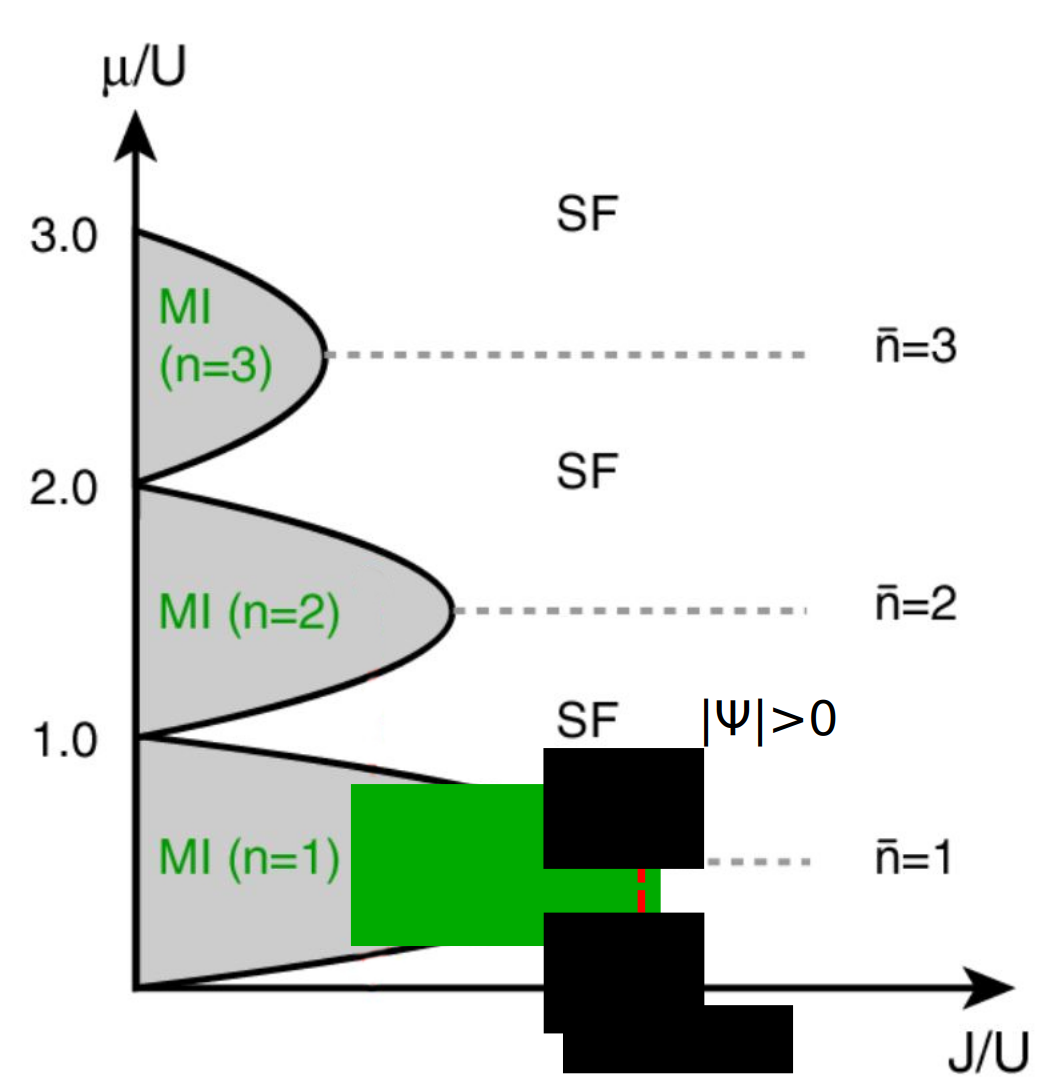
\includegraphics[width = 0.5\textwidth]{Figures/SFMottPhase.pdf}
	\label{fig:SFMOTT}
	\caption{\textit{Phase diagram of Bose-Hubbard model for T = 0. Grey areas mark the Mott Insulator phase for different number of particles per site, while white regions mark the superfluid phase. \cite{greiner}}}
\end{figure}
The $\mu_{\pm}$ curves encloses the region where the system is in the Mott Insulating phase. $(1/\bar{U})_{crit} = (J/U)_{crit}$ can be read off the graph from the point, where the two curves $\mu_{\pm}$ meet. As mentioned earlier, no fluctuations take place in the Mott Insulator, whereby the particle number per site is well defined, while it for the superfluid can take many values. As the chemical potential increases each site can accommodate more particles as long as the increase in chemical potential compensates the increased energy due to interactions between the particles.\\
The mean-field solution of the Bose-Hubbard model is only an approximation, which proves quite inaccurate for one dimension. This is seen when comparing the critical ratio for the mean-field approach, $\left( U/J \right)_{crit}^{MF,1D} = 11.66$, with numerical results computed using the DMRG method, $\left( U/J \right)_{crit}^{DMRG,1D} = 3.37$, \cite{Kuhner2000}. Nevertheless, it gives a good intuitive feeling of the physics taking place and how one can describe them without resorting to diagonalizing the Hamiltonian.\\
\chapter{Quantum Optimal Control Theory}
The fundamental problem of Quantum Optimal Control Theory is to steer the dynamics of a quantum system in a desired way through external fields \cite{Rice2000,Shapiro2003}. Often, the goal is the transfer from an initial state, $\ket{\psi_0}$, to the desired target-state, $\ket{\psi_{\mathrm{target}}}$. The fields responsible for controlling the dynamics of the system are parametrised by a set of control parameters or functions. Optimal control theory determines the parameters, which leads to the desired dynamics of the system \cite{Werschnik2007}.\\ 
In control problems, the Hamiltonian of the system is given as
\begin{equation}
	\hat{H} = \hat{H}_0 + \hat{H}_I = \hat{H}_0 + \sum_{n = 1}^{m}  \hat{H}_n (u_n(t)) \; ,
	\label{eq:ControlHamiltonians}
\end{equation} 
where $\hat{H}_0$ is an uncontrollable drift of the Hamiltonian, $\hat{H}_n$ are the controllable fields, and $u_n(t)$ are the control functions or parameters. A quantum system like this is completely controllable if every unitary operator $\hat{U}$ is accessible from the identity operator $\hat{I}$ via a path $\gamma (t) = \hat{U}(t, t_0)$ satisfying \cite{Schirmer2001}
\begin{equation}
	i \partial_t \hat{U}(t, t_0) = \left( \hat{H}_0 + \hat{H}_I \right) \hat{U}(t, t_0) \; .
\end{equation} 
For an $N$-dimensional Hilbert spaces, a sufficient condition for complete controllability of a quantum system is that the Lie algebra generated by the Hamiltonians in eq. \eqref{eq:ControlHamiltonians},
\begin{equation}
	L_0 = \mathrm{Lie} \left( i \hat{H}_0, i \hat{H}_1 , \ldots , i \hat{H}_m \right) \; ,
\end{equation}
is of dimension $N^2$ \cite{Ramakrishna1995}.\\
Extending these conditions to infinite-dimensional Hilbert spaces and constrained controls is non-trivial \cite{Huang1983}. Therefore, no calculations of the Lie dimensions will be performed for the control problems presented in this thesis.


\section{The Gradient-Ascent Pulse Engineering Method - GRAPE} \label{sec:GRAPE}
The control problem presented in this thesis is steering the system from an initial state in the Superfluid phase to a target-state in the Mott-Insulator phase. This is achieved by varying the lattice depth, which therefore can be considered the control parameter. Hence, the optimal control problem can be stated as follows: 
Suppose the system is initially described by the state $\ket{\psi_0} = \ket{\psi (0)}$, and the potential is varied in the time interval $[ 0 , T]$. The goal is finding the set of control parameters, $\boldsymbol{u}(t)$, which brings the initial state as close as possible to the target state, $\ket{\psi_{\mathrm{target}}}$. This is formulated in terms of a cost function
\begin{equation}
	J_T = \frac{1}{2} \left( 1-|\braket{\psi_{\mathrm{target}} | \psi (T)}|^2 \right) \; ,
	\label{eq:infidelityCost}
\end{equation}
which is given as half the infidelity between the target and the state at $t=T$. The cost function becomes zero, when the terminal state matches the target state up to an arbitrary phase. Hence, the optimal control problem can be formulated as a minimization problem of eq. \eqref{eq:infidelityCost} \cite{Jager2014}.\\
Experimentally, large variations in the control parameter is often hard to achieve. Therefore, an extra term is often added to the cost function, which penalizes strong variations in the control. The new cost function reads
\begin{equation}
	J = J_T + J_R = J_T + \frac{\gamma}{2} \sum_{n=1}^{m} \int_{0}^{T} \left( \pdv{u_n}{t} \right)^2 \mathrm{d}t \; ,
	\label{eq:grapeCost}
\end{equation}
where $\gamma$ weighs the relative importance between matching states and smoothness of the control \cite{Jager2014}. As the state transfer is considered the highest priority, $\gamma$ is set as $\gamma \ll 1$, such that $J_T$ dominates the cost function of eq. \eqref{eq:grapeCost}.\\

A powerful way of performing optimal control is through the Gradient-Ascent Pulse Engineering (GRAPE) method. Through GRAPE, the gradient of the cost function \eqref{eq:grapeCost} can be evaluated and used to update the existing set of controls \cite{Khaneja2005}. Thereby, one achieves an optimization of the cost function.\\
The gradient of the cost function can be derived in multiple ways. A common method \cite{Hohenester2007, Winckel2008, BECcontrol} is introducing a Lagrange multiplier, which forces the dynamics to obey the Schrödinger equations. The derivation utilizes functional derivatives, as time, $\ket{\psi (t)}$, and the Lagrange multiplier are considered continuous functions. Later, the functions are discretized to perform numerical computations. Although this procedure is fairly easy, higher order correction terms of the gradient are absent due to the continuity of the functions. Here, an alternative derivation following \cite{Khaneja2005, deFouquieres2011} is presented in which the discretization is introduced immediately. \\
Assume the transfer time, $T$, is discretized in $M$ equal steps, $\Delta t = T/M$. Therefore, the control become similarly discretized as
\begin{equation}
	u_n = \left( u_n (t_1) , \ldots , u_n (t_M)  \right) \equiv \left( u_n (1) , \ldots , u_n (M)  \right) \; .
\end{equation}
Likewise, the time-evolution of the system during the time step $j$ is given by the propagator
\begin{equation}
	\hat{\mathcal{U}}_j \equiv \hat{\mathcal{U}} (u(t_j)) = \exp \bigg\{ -i \left(  \sum_{n = 1}^{m}  \hat{H}_n (u_n(j))  \right) \Delta t \bigg\} \; . 
\end{equation} 
Thereby, the cost function \eqref{eq:grapeCost} becomes
\begin{equation}
	J = \frac{1}{2} \left( 1 - |\braket{\psi_{\mathrm{target}} | \prod_{j = 1}^{M} \hat{\mathcal{U}}_j | \psi (0)}|^2 \right) + \frac{\gamma}{2} \sum_{n = 1}^{m} \sum_{j = 1}^{M-1} \left( \frac{\Delta u_n (j)}{\Delta t} \right)^2 \Delta t \; ,
	\label{eq:discreteCost}
\end{equation}
where $\Delta u_n (j) =  u_n (j+1) - u_n (j)$. The full gradient of the cost, $\nabla J(\boldsymbol{u})$, is a vector of partial derivatives $\frac{\partial J(\boldsymbol{u})}{\partial u_n (j)}$.\\
First, consider the derivative of the regularization
\begin{align}
	\frac{\partial J_R}{\partial u_n (j)} &= \frac{\gamma}{2} \left( 2 \frac{u_n (j) - u_n (j-1)}{\Delta t^2} - 2 \frac{u_n (j+1) - u_n (j)}{\Delta t^2} \right) \Delta t \nonumber \\
	&= \frac{\gamma}{\Delta t} \left( 2 u_n (j) - u_n (j+1) - u_n (j-1) \right) \; . \label{eq:regularizationGrad}
\end{align}
The part of the gradient related to the regularization depends only on the control, whereby it can be calculated without considering the state of the system.\\ 
Next, consider the derivative of $J_T$. Defining the transfer probability amplitude $\tau \equiv \braket{\psi_{\mathrm{target}} | \psi (T)}$, the derivative of the final infidelity with respect to the control can be written as 
\begin{equation}
	\frac{\partial J_T}{\partial u_n (j)} = - \frac{1}{2} \frac{\partial}{\partial u_n (j)}  \tau^* \tau   = - \Re \left( \tau^* \frac{\partial \tau}{\partial u_n (j)} \right) \; .
	\label{eq:dJTdu}
\end{equation}
From eq. \eqref{eq:dJTdu} it is evident that the derivative of the infidelity only depends on the derivative of the transfer probability amplitude, $\frac{\partial \tau}{\partial u_n (j)}$. This derivative can be rewritten as
\begin{align}
	\frac{\partial \tau}{\partial u_n (j)} &= \frac{\partial }{\partial u_n (j)} \braket{\psi_{\mathrm{target}} | \prod_{j = 1}^{M} \hat{\mathcal{U}}_j | \psi (0)} \nonumber \\
	&= \bra{\psi_{\mathrm{target}}} \hat{\mathcal{U}}_M \ldots \hat{\mathcal{U}}_{j+1} \frac{\partial \hat{\mathcal{U}}_{j}}{\partial u_n (j)} \hat{\mathcal{U}}_{j-1} \ldots \hat{\mathcal{U}}_{1} \ket{\psi (0)}
	\label{eq:dcdu}
\end{align}
Multiplying eq. \eqref{eq:dcdu} with $\tau^*$ to recreate the result of eq. \eqref{eq:dJTdu} yields
\begin{align}
	\tau^* \frac{\partial \tau}{\partial u_n (j)} &=  \braket{\psi(T) | \psi_{\mathrm{target}}} \Braket{\psi_{\mathrm{target}} | \prod_{j' = j +1}^{M} \hat{\mathcal{U}}_{j '} \frac{\partial \hat{\mathcal{U}}_{j}}{\partial u_n (j)} \prod_{j' = 1}^{ j-1} \hat{\mathcal{U}}_{j '} | \psi (0)} \\
	&= i \Braket{\chi (T) | \prod_{j' = j +1}^{M} \hat{\mathcal{U}}_{j '} \frac{\partial \hat{\mathcal{U}}_{j}}{\partial u_n (j)} \prod_{j' = 1}^{ j-1} \hat{\mathcal{U}}_{j '} | \psi (0)} \\
	&= i \Braket{\chi (t_j) |  \frac{\partial \hat{\mathcal{U}}_{j}}{\partial u_n (j)} | \psi (t_{j-1})} \; ,
	\label{eq:gradientForBack}
\end{align}
where $\ket{\chi (T)} \equiv i \ket{\psi_{\mathrm{target}}} \braket{\psi_{\mathrm{target}} | \psi (T)}$ is the projection of the final state unto the target state. Notice how in eq. \eqref{eq:gradientForBack} the state $\ket{\chi (T)}$ has been propagated backwards in time.\\ 
The derivative of the propagator, $\hat{\mathcal{U}}_{j}$, is non-trivial, due to possible non-commutativity between the Hamiltonian and its derivative. This results in a series of higher order corrections to the derivative of propagator.
Expanding the propagator as a Taylor series before taking the derivative gives
\begin{align}
	\frac{\partial \hat{\mathcal{U}}_{j}}{\partial u_n (j)} &= \frac{\partial}{\partial u_n (j)}  \exp \left( -i \hat{H} \Delta t \right) \nonumber \\
	&= \sum_{p = 0}^{\infty} \frac{( -i \Delta t  )^p}{p!} \frac{\partial \hat{H}^p}{\partial u_n (j)} \; .  
	\label{eq:derivTaylorExp}
\end{align}
As mentioned before the Hamiltonian may not commute with its derivative. Therefore, one must be careful when taking the derivative of $\hat{H}^p$. Retaining the ordering of the operators while taking the derivative yields
\begin{align}
	\frac{\partial \hat{\mathcal{U}}_{j}}{\partial u_n (j)} &= \sum_{p=1}^{\infty} \frac{ \left( -i \Delta t \right) ^p }{p!} \sum_{q=0}^{p-1} \hat{H}^q \frac{\partial \hat{H}}{\partial u_n (j)} \hat{H}^{p-q-1} \nonumber \\
	&= \sum_{p=0}^{\infty} \sum_{q=0}^{\infty} \frac{A^p B A^q}{(p+q+1)!} \; , \label{eq:derivTaylorExp2}
\end{align} 
where $A = -i \hat{H} \Delta t$ and $B = -i \partial \hat{H}/\partial u_n (j) \Delta t$ have been defined for notational convenience. Through the standard relations of the gamma function, $\Gamma (z)$, one can derive the identity
\begin{equation}
	\frac{1}{(p+q+1)!} = \frac{1}{p! q !} \int_{0}^{1} (1-\alpha)^p \alpha^q \mathrm{d}\alpha \; .
\end{equation}
Thereby eq. \eqref{eq:derivTaylorExp2} can be expressed as
\begin{align}
	\frac{\partial \hat{\mathcal{U}}_{j}}{\partial u_n (j)} &= \sum_{p=0}^{\infty} \sum_{q=0}^{\infty} \frac{A^p B A^q}{p! q !}  \int_{0}^{1} (1-\alpha)^p \alpha^q \mathrm{d}\alpha \nonumber \\
	&= \int_{0}^{1} \sum_{p=0}^{\infty} \sum_{q=0}^{\infty} \frac{(A (1- \alpha))^p}{p!} B \frac{(A \alpha)^q}{q!}  \mathrm{d}\alpha \nonumber \\
	&= \int_{0}^{1} e^{ (1- \alpha) A} B e^{ \alpha A} \mathrm{d}\alpha \nonumber \\
	 &= e^A \int_{0}^{1} e^{ - \alpha A} B e^{ \alpha A} \mathrm{d}\alpha \; , \label{eq:eq:derivTaylorExp3}
\end{align}
where the expansion of the exponential function has been used to eliminate the sums. Although eq. \eqref{eq:eq:derivTaylorExp3} looks rather simple, however, evaluating the integral in its current form is a fairly hard task. Instead, the integral can be explicitly solved by applying the Baker–Campbell–Hausdorff expansion 
\begin{equation}
	e^X Y e^{-X} = \sum_{k = 0}^{\infty} \frac{ [ X,Y  ]_k }{k!} = Y + [ X,Y  ] + \frac{1}{2!} [ X , [ X,Y  ]] + \frac{1}{3!} [X, [ X , [ X,Y  ]]  ] + ...
\end{equation}
where $[ X , Y ]_k = [ X ,[ X , Y]]_{k-1}$ and $[X,Y]_0 = Y$ is the definition of the recursive commutator \cite{Wilcox1967}. Thus, eq. \eqref{eq:eq:derivTaylorExp3} reads
\begin{align}
	\frac{\partial \hat{\mathcal{U}}_{j}}{\partial u_n (j)} &=  e^A \int_{0}^{1} \sum_{k = 0}^{\infty } \alpha^{k+1} \frac{(-1)^k}{k!} [ A,B  ]_k \mathrm{d}\alpha \nonumber \\
	&= e^A  \sum_{k = 0}^{\infty }  \frac{(-1)^k}{(k+1)!} [ A,B  ]_k \; .
\end{align}
Inserting this final expression for the derivative of the propagator into eq. \eqref{eq:dJTdu}, one finds the exact derivative of the infidelity 
\begin{align}
\frac{\partial J_T}{\partial u_n (j)} &=  - \Re  \Braket{\chi (t_j) | i e^{-i \hat{H} \Delta t}  \sum_{k = 0}^{\infty }  \frac{(-1)^k}{(k+1)!} \left[ -i \hat{H} \Delta t , -i \frac{\partial \hat{H}}{\partial u_n (j)} \Delta t  \right]_k | \psi (t_{j-1})}  \nonumber \\
	&=  - \Re  \Braket{\chi (t_{j-1}) | \sum_{k = 0}^{\infty }  \frac{i^{k+1} \Delta t^{k+1}}{(k+1)!} \left[ \hat{H} , \frac{\partial \hat{H}}{\partial u_n (j)}  \right]_k | \psi (t_{j-1})}  \; . \label{eq:higherOrderGradient}
\end{align}
For small time-steps the higher order corrections can be neglected, however, choosing a larger time-step reduces the run-time of the time-evolution, which is critical when describing many-body systems. Therefore, including higher order contributions increases the accuracy, whereby larger time-steps can be employed. Computing the higher order corrections can be done efficiently by analytically deriving the commutators beforehand. The increase in accuracy achieved depends on the system, as it is determined by the commutator $[ \hat{H} , \partial \hat{H} / \partial u_n (j) ]$ and how the propagator, $\hat{\mathcal{U}}_{j}$, is constructed. In section \ref{sec:modTMDRG} an alternative propagator is constructed using the Suzuki-Trotter expansion, which causes the gradient to be exact to zeroth order.\\
Finally, combining the derivatives of eq. \eqref{eq:regularizationGrad} and \eqref{eq:higherOrderGradient} produces the entries of the gradient vector for the cost function
\begin{equation}
	\frac{\partial J (\boldsymbol{u})}{\partial u_n (j)}  = - \Re \Braket{\chi (t_{j-1}) | \left( i \frac{\partial \hat{H}}{\partial u_n (j)} \Delta t + \mathrm{h.o.} \right)  | \psi (t_{j-1})}  + \frac{\gamma}{\Delta t} \left( 2 u_n (j) - u_n (j+1) - u_n (j-1) \right) \; .
	\label{eq:costGradient}
\end{equation}
Here $\mathrm{h.o.}$ denotes all higher order terms ($k > 0$).\\ 

Through the analytically derived gradient, the cost can be iteratively updated using gradient-based optimization methods until a desired threshold is reached. This forms the framework of the Gradient-Ascent Pulse Engineering (GRAPE) algorithm \cite{Khaneja2005}, which is summarised below:

\begin{algorithm}
\begin{algorithmic}
\caption{GRAPE Algorithm}
\State Choose initial control $\boldsymbol{u}^{(1)}$.
\While{$ J > J_{\mathrm{threshold}}$}
	\State Calculate $\ket{\psi (t_k)} = \prod_{j=1}^{k} \hat{\mathcal{U}}_j \ket{\psi (0)}$ for $k = 1 \ldots M$.
	\State Calculate $\ket{\chi (t_k)} = \prod_{j=M}^{k} \hat{\mathcal{U}}_{j}^{\dag} \ket{\chi (T)}$ for $k = M \ldots 1$. 
	\State Evaluate $\frac{\partial J}{\partial u_n (k)}$ for $k = 1 \ldots M$ and $n = 1 \ldots m$ according to eq. \eqref{eq:costGradient}.
	\State Update controls using gradient such that $J^{(i + 1)} < J^{(i)}$. 
\EndWhile
\end{algorithmic}
\end{algorithm}
The computations are performed under the boundary conditions
\begin{align}
	\boldsymbol{u}(0) &= \text{fixed value} \label{eq:firstBound} \\
	\boldsymbol{u}(T) &= \text{fixed value} \\
	\ket{\psi (0)} &= \ket{\psi_0} \\
	\ket{\chi (T)} &= -i \ket{\psi_{\mathrm{target}}} \braket{\psi_{\mathrm{target}} | \psi (T)} \; .  \label{eq:lastBound}
\end{align}
Figure \ref{fig:ControlUpdate} illustrates an update step of the controls such that the cost function is reduced.
\begin{figure}[!h]
	\centering
	\includegraphics[width=0.7\columnwidth]{Figures/ControlUpdate.pdf} 
	\caption{ \textit{Visualisation of update step $i \to i+1$ the control $\boldsymbol{u}^{(i)}$ resulting in a decreased cost function.}}
	\label{fig:ControlUpdate} 
\end{figure} 
Although the starting guess of the control, $\boldsymbol{u}^{(1)}$, can be completely random, both faster convergence and lower convergence value is achieved by choosing a good starting seed. Clearly, there is no guarantee that the algorithm will converge to the global optimum, as it is based on a gradient ascent procedure \cite{Khaneja2005}. Nevertheless, the algorithm can be made to search a large portion of the parameter space by executing it multiple time for various seeds.  


\section{Gradient-Optimization Using Parametrization - GROUP} \label{sec:GROUP}
The convergence rate of optimal control sequences has been shown to be greatly improved by employing gradient-based methods, such as GRAPE, for updating the control \cite{Jager2014}.
One of the disadvantages of GRAPE is the dimension for the optimization. As the duration of the control pulse is discretised into $M$ time-steps, the control at each of these steps must be optimized. For long durations or small time-steps the resulting dimension of the optimization ($M$) will be very large. One can consider this type of control parametrisation having too many degrees of freedom for the optimization. 
However, by employing a proper parametrisation of the control, the optimization dimension can be drastically reduced \cite{Winckel2008}.\\
The typical choice is employing a chopped basis, which parametrises the control as
\begin{equation}
	u(t) = u_0 (t) + S(t) \sum_{n=1}^{N} c_n f_n (t) \; , \label{eq:controlParametrization}
\end{equation}   
where $f_n$ are the basis functions. In addition, $u_0 (t)$ is the initial control function, and $S (t)$ is a shape function enforcing the boundary conditions of the control, whereby $S(0) = S(T) = 0$ CITE JJ ARTIKEL. The shape function used throughout this thesis consists of two steep sigmoids oriented such that $S$ is unit for most time steps. In the chopped basis the coefficients $c_n$ are optimized rather than the full control, $u(t)$. The basis functions, $f_n$, must be chosen based on physical insight of the system. For the control problem discussed in this thesis, employing a basis of sine functions has proven itself useful, as the sine functions are excellent at describing the smoothly varying control pulses desired CITE JJ. Thus, the basis functions read $f_n = \sin \left( \frac{\omega_n t}{T} \right)$, where $\omega_n = n \pi$.
An extension of this type of chopped basis was done in \cite{Doria2011,Caneva2011}, introducing random shifts to the frequencies resulting in the Chopped RAndom Basis or \textsc{CRAB}. In recent years the \textsc{CRAB} parametrisation has been used together with the Nelder-Mead hill climbing algorithm to solve various control problems \cite{Doria2011,Caneva2011,FrankBloch,Lloyd2014}.\\
The great advantage of employing a reduced basis representation is the drastic reduction in the optimization space, whereby the optimal control can be found much more efficiently. However, artificial minima can be introduced, if the chosen basis is incapable of spanning the part of the optimization space containing the optimal solutions \cite{Rach2015}. Hence, the chopped basis dimension, $N$, must be chosen not too small.\\

The Gradient-Optimization Using Parametrization or \textsc{GROUP} algorithm introduced in JJ CITE combined the chopped basis representation with the gradient based \textsc{GRAPE} algorithm. This of course alters the gradient of the cost functional described in eq. \eqref{eq:costGradient}. The new gradient can be derived using the chain rule
\begin{align}
	\frac{\partial J (\boldsymbol{c})}{\partial c_n} &= \sum_{m = 1}^{M} \frac{\partial J }{\partial u(t_m)} \frac{\partial u(t_m)}{\partial c_n} \nonumber \\
	&= \sum_{m = 1}^{M} \frac{\partial J }{\partial u(t_m)} S(t_m) f_n(t_m) \; , \label{eq:GROUPgradient} 
\end{align}
where only a single control, $u$, has been chosen for cleaner notation. The gradient in \textsc{GROUP} is more complicated than in \textsc{GRAPE} ($\frac{\partial J }{\partial u(t_m)}$, see eq. \eqref{eq:costGradient}). However, the cost of computing the gradient is still dominated by the evaluation of $\frac{\partial J }{\partial u(t_m)}$, as this requires two time-evolutions for the full duration, $T$. Therefore, the chopped basis representation reduces the dimension of the optimization space, thereby reducing the number of elements in the cost gradient, while causing a negligible increase in the computational difficulty of computing the gradient.
In JJREF a comparison between different optimization algorithms for optimal control showed that \textsc{GROUP} outperformed both \textsc{GRAPE} and Nelder-Mead with \textsc{CRAB} in term of fidelity reached and number of function evaluations required.

\subsection{Alteration of constraints through GROUP}
Although GROUP drastically reduces the number of optimization parameters, it comes with the cost of a large increase in constraints.\\
Consider the non-parametrized optimization problem discretized in time. In this case the problem is subjected to the boundaries of eq. \eqref{eq:firstBound}-\eqref{eq:lastBound}. Furthermore, a set of constraints of the control is often needed. Consider the specific case of the control system being a lattice system described by the Bose-Hubbard model and the control being the lattice depth. A minimum value of the control is required, as the lattice depth must be near the tight-binding limit for the model to remain a good description of the system. This constraint must be enforced at all times. In addition to this, an upper limit of the control may be desired to restrict the interval in which the solution is searched for. Thus, the constraints of the optimization problem reads 
\begin{equation}
	 u_{min} \geq u(i) \geq u_{max} \quad \forall i \; .
\end{equation}

Employing the GROUP algorithm causes a parametrization of the control, eq. \eqref{eq:controlParametrization}, which in turn alters the constraints. Most gradient-based optimization algorithms require the Jacobian of the constraints in addition to the gradient of the objective function. Interior point methods, which is the algorithm of choice for solving the control problems described in this thesis, are without exception. Thus, one must also consider the alteration of the Jacobian, which has elements of the general form $\boldsymbol{J}_{ij} = \frac{\partial f_i}{\partial x_j}$.
Since the constraint function is simply the time discretized control itself, the Jacobian is given by
\begin{equation}
	\boldsymbol{J}_{ij} = \frac{\partial u(i)}{\partial c_j} = S(i) f_j (i) \; .
\end{equation}
Thus, the Jacobian of the constraints has $M * N$ entries, where $M$ is the number of time steps, and $N$ is the dimension of the optimization space. However, these elements are fast to retrieve, as they remain constant throughout the optimization. 


\section{Interior Point Method} \label{sec:IntPoint}
Through the gradient of the cost functional, the control functions can be iteratively updated yielding an improved cost. The update of the control functions can be done using various hill-climbing methods.
Interior point methods are modified versions of Newtons method for bound, constrained problems. The methods approach the solution from within the feasible region and provides efficient performance while having better theoretical properties than the standard simplex method \cite{wright}.\\

Here, a linear version of the method will be derived, however, the formalism can easily be extended to non-linear problems \cite{wright}.
Consider the general minimization problem
 \begin{align*}
	\min_{x \in \mathbb{R}^n} \;  & \; c^T x \\
	\text{subject to} \;  & \; A x = b  \\
							& \; x \geq 0 \; ,
\end{align*}
which can be derived from any linear problem through slack variables that transform inequality constraints into equality constraints at the cost of introducing extra variables \cite{ipopt}.

\subsection{Karush–Kuhn–Tucker conditions}
A central concept in mathematical optimization is the Karush–Kuhn–Tucker (KKT) conditions, which are first-order conditions for a solution of a nonlinear problem to be an optimum. The KKT conditions allow inequality constraints, whereby they are more general than Lagrange multipliers. 
\begin{theorem}
	Suppose that $x^*$ is a local solution of the objective function $f \; : \; \mathbb{R}^n \to \mathbb{R}$ with respect to a collection of constraints $\{ c_i(x)  \}_{i=1}^{m}$, where $c_i \; : \; \mathbb{R}^n \to \mathbb{R}$. Let $\mathcal{L}$ be the Lagrangian of the problem. If the subset of the equality constraints $\{ c_i(x) \in \mathcal{E}\}$ has the property that $\{ \nabla c_i(x^*)\}$ is linear independent, then a vector of Lagrange multipliers, $\lambda^*$, exists for which the following holds:
	\begin{subequations}	
	\begin{align}
		\nabla_x \mathcal{L}(x^*,\lambda^*) &= 0 \; ,  \\
		c_i(x^*) &= 0 \; , \qquad \forall i \\
		\lambda_{i}^* &\geq 0 \; , \qquad \forall i \in \mathcal{I} \\
		\lambda_{i}^* c_i(x^*) &= 0 \; , \qquad \forall i \in \mathcal{E} \cup \mathcal{I}
	\end{align}
	\end{subequations}	
	where $\mathcal{E}$ and $\mathcal{I}$ denote the equality and inequality subspaces respectively \cite{wright}.  
\end{theorem}
The KKT conditions is a way of determining, whether a point is an optimum. If $x^*$ satisfies the conditions, its objective value must be lower than the objective point of any other point.


\subsection{Barrier Problems}
In interior point methods the boundaries of the variables are enforced through a barrier function, which keeps the objective function continuously differentiable.
A general, linear optimization problem can be associated with a barrier function
\begin{equation}
	B(x , \mu) = c^T x - \mu \sum_{i=1}^{n} \ln x_i \; ,
\end{equation} 
where the barrier parameter $\mu > 0$. For $\mu \to 0$ one recovers the original problem.
The optimization Lagrangian of the barrier problem is
\begin{equation}
	\mathcal{L}(x, \lambda, s) = c^T x - \mu \sum_{i=1}^{n} \ln x_i - \lambda^T (A x -b) \; ,
\end{equation}
where $\lambda \in \mathbb{R}^m$ is the Lagrange multiplier for the $A x = b$ constraint. Now, let $X = \mathrm{Diag}(x_1 , \ldots , x_n)$, $e = (1,1, \ldots , 1)^T$, $s = \mu X^{-1} e$, and $S = \mathrm{Diag}(s_1 , \ldots , s_n)$. Thereby the KKT conditions of the barrier problem can be stated as 
\begin{subequations}
\begin{align}
	A^T \lambda + s &= c \\
	A x &= b \\
	X S e &= \mu e \; .
\end{align}
\end{subequations}
By adding the barrier term the KKT complementary condition has been "relaxed", as it is no longer equals zero \cite{ipnote}. Again, for $\mu \to 0$ the original conditions are recovered. 


\subsection{Primal-Dual Interior Point Method}
Primal-dual methods optimize an additional, \textit{dual}, problem while optimizing the main, \textit{primal}, problem.
Consider the initial linear problem. Its dual is defined as 
\begin{align*}
	\max_{\lambda \in \mathbb{R}^n} \;  & \; b^T \lambda \\
	\text{subject to} \;  & \; A^T \lambda + s = c  \\
							& \; s \geq 0 \; .
\end{align*}
If either the primal or the dual problem has a solution, then so does the other, and the objective values are equal. If either problem is unbounded, then the other problem is infeasible. If a solution exists, then the optimal solution to the dual problem are the Lagrange multipliers to the primal problem and vice versa \cite{wright}. Note, how the dual of the dual problem is the original problem.
Hence, for primal-dual algorithms triplet of variables, $(x , \lambda , s)$, is considered when computing the optimum of a function.\\

The primal-dual interior point method computes a constrained Newton step, which is used to iterate the variables towards the optimum. Thisis done by solving a primal-dual barrier problem for a given $\mu$, yielding the optimum solution of said subproblem. The optimal solution of the main problem is found by solving these subproblems iteratively for ever decreasing $\mu$ using the previous solution as starting point \cite{ipopt}.\\
The solutions for the primal-dual subproblems are characterized by the KKT conditions. These conditions can be written into a single mapping
 \begin{align}
    F(x , \lambda, s) &= \begin{pmatrix}
           A^T \lambda + s - c \\
           A x - b \\
           X S e
         \end{pmatrix} = 0
  \end{align}
  which has the Jacobian
 \begin{align}
    J(x , \lambda, s) = \begin{pmatrix}
           0 & A^T & I	\\
           A & 0 & 0 	\\
           S & 0 & X
         \end{pmatrix}
  \end{align}
Thus, the Newton direction, $(x_B , \lambda_B , s_B)$, can be written as the solution to the system of equations
\begin{align}
J \begin{pmatrix}
           x_B \\
           \lambda_B \\
           s_B
         \end{pmatrix} = -F
\end{align}
This equation does not take into account the barrier function, however, as stated earlier, the effect of the barrier term is to relax the the KKT complementary condition. This is achieved by setting $X S e = \mu e$, whereby one obtains
\begin{align}
	\begin{pmatrix}
    	 0 & A^T & I    \\
         A & 0 & 0 		\\
         S & 0 & X
    \end{pmatrix} 
    \begin{pmatrix}
    	x_b 		    \\
        \lambda_B		\\
        s_B
    \end{pmatrix} =
    - \begin{pmatrix}
    	  A^T \lambda + s - c 	\\
          A x - b 				\\
          X S e - \mu e
    \end{pmatrix} \; . \label{eq:newtondirection}
\end{align}
Thereby the parameters can be iteratively updated through the calculated Newton direction
\begin{equation}
	(x_{k+1} , \lambda_{k+1} , s _{k+1}) = (x_{k} , \lambda_{k} , s _{k}) + \alpha  (x_B , \lambda_B , s_B) \; , \label{eq:newtonstep}
\end{equation}
where $\alpha$ can be found using a line-search or other more sophisticated methods.
The procedure above can be summarized in the following algorithm \cite{ipnote}:\\
\begin{algorithm}
\begin{algorithmic}
\caption{Primal-Dual Interior Point Algorithm}
\State Choose $\sigma \in (0,1)$ and $\mu_0 > 0$.
\State Choose initial point $(x_0 , \lambda_0 , s_0)$ within feasible region.
\For{$k = 1 , \ldots$}
	\State $\mu_k \gets \sigma \mu_{k-1}$
	\State Calculate the Newton direction using eq. \eqref{eq:newtondirection}.
	\State Compute step-size $\alpha$.
	\State Update parameters according to eq. \eqref{eq:newtonstep}
\EndFor
\end{algorithmic}
\end{algorithm}

The implementation of the interior point algorithm used in this thesis is from the IPOPT library \cite{Wachter2006}, which also approximates the Hessian of the optimization Lagrangian through previous derivatives using the L-BFGS algorithm \cite{Liu1989}. By including information about the second derivative, the algorithm is able to converge in much fewer iterations. 


\section{Quantum Speed Limit}
A subtlety of optimal control problems is that one is only searching for the control, $\boldsymbol{u}(t)$, which steers the initial state into the target-state at time $t = T$. It is often desirable to obtain the desired state in the shortest timespan possible. However, if a solution exists at $t= T_1$, it might not exist at $t = T_2 < T_1$. The shortest duration for which a solution can be found is called the \textit{quantum speed limit} (QSL). A large energy difference to orthogonal states allows for fast oscillations within a system, however, these differences cannot be arbitrarily large. Hence, a lower bound of how fast a system can evolve exists, which in turn leads to the QSL \cite{Caneva2009}.\\
There are several ways of approximating the quantum speed limit, however, there is no known way to reliably determine the QSL for a general state. Therefore, the best option is often to just solve the problem at increasingly shorter durations, until a solution no longer can be found [JJ].\\
If the initial state, $\ket{\psi_0}$, and the target-state, $\ket{\psi_{\mathrm{target}}}$, are orthogonal, one can estimate the QSL from the orthogonalization time, which is how long it takes for a state to become orthogonal to itself.
Consider $\ket{\psi (0)} = \sum_{n}^{\infty} c_n \ket{\phi _n}$, where $\hat{H} \ket{\phi _n} = E_n \ket{\phi _n}$. Following \cite{QSLtoffoli}, the norm squared of the survival probability is given as
\begin{align}
	|S(t)|^2 = |\braket{\psi (0) | \psi (t)}|^2 &= \sum_{n , m = 0}^{\infty} |c_n|^2 |c_m|^2 \cos \left( (E_n - E_m) t \right) \nonumber \\
	&\geq 1 + \frac{4 t}{\pi ^2} \dv{|S(t)|^2}{t} - \frac{4 t^2}{\pi} \Delta E^2 \; ,
\end{align}
where the trigonometric inequality $\cos x \geq 1 - \left( 4 x \sin x - 2 x^2 \right) / \pi^2$ was used, and $\Delta E$ is the energy spread of the state.
Since $|S(t)|^2 \geq 0$, then $\dv{|S(t)|^2}{t} = 0$ whenever $|S(t)| = 0$, which is the case at the orthogonalization time $t = \tau$. This leaves the inequality $0 \geq 1 - 4 \tau^2 \Delta E^2 / \pi^2$, yielding the Mandelstram Tamm bound when solved \cite{Mandelstam1991}
\begin{equation}
	\tau_{\mathrm{MT}} \geq \frac{\pi}{2 \Delta E} \; .
	\label{eq:MandelstamBound}
\end{equation}
Eq. \eqref{eq:MandelstamBound} sets a lower bound of the orthogonalization time, however, the bound was derived using a constant Hamiltonian. In the case of optimal control, the Hamiltonian is time dependent, which can be taken into account by using arguments from differential geometry \cite{Aharonov,beyondQSL}
\begin{equation}
	\tau_{\mathrm{MT}} \geq \frac{\pi}{2} \left( \int_{0}^{T} \Delta E \; \mathrm{d}t \right) ^{-1} \; , \label{eq:MTlimit}
\end{equation}
Equations \eqref{eq:MandelstamBound} and \eqref{eq:MTlimit} show how fast solutions require a large value of $\Delta E$. Since \ref{eq:MTlimit} is dependent on the control $\boldsymbol{u}(t)$, one would have to take an infimum over all controls connecting the initial and target state in order to evaluate the lowest value of the bound. This in itself is a task just as difficult as solving the control problem.\\
For an example of optimal control see Appendix \ref{chap:LZexample}, which illuminates some of the consequences of the quantum speed limit.
\chapter{Matrix Product States}
Attempts to perform numerical analysis of quantum many-body systems using exact diagonalisation are highly limited by system sizes. Due to the large number of possible configurations in a many-body scenario and entanglement coupling various degrees of freedom of the system, the Hilbert space grows too large for exact methods to search.
Consider the Bose-Hubbard model described in eq. \eqref{BHhamil}. The dimension of the corresponding Hilbert space is
\begin{equation}
	D_{\mathcal{H}} = \frac{(N+N_p -1)!}{N_p ! (N-1)!} \; ,
\end{equation}
where $N$ is the number of sites, and $N_p$ is the number of particles. For unit occupancy, $N_p / N = 1$, the Hilbert space grows exponentially with the system size \cite{Dong}. Therefore, descriptions using exact diagonalisation are only possible for small systems.
The invention of the density-matrix renormalization group
(DMRG) marked a turning point for numerical descriptions of quantum many-body systems, as it remains the most powerful method to study one-dimensional lattices \cite{White1992,White1993}. One of the defining differences between the DMRG method and exact diagonalisation is scaling of entanglement in the quantum states. In the DMRG description, systems automatically follow an area law, whereby only a tiny corner of the Hilbert space has to be considered when searching for ground states \cite{Cramer}.\\
Matrix Product States (MPS) are parametrizations of (typically) one dimensional states, where the states and operators are decomposed into networks of tensors. In this description of quantum states it is very easy to measure local properties of quantum many-body systems, and correlations can be computed very efficiently. The matrix product state description has surfaces several times under different names, most notable in \cite{Baxter1968}. However, the connection between the DMRG method and the MPS description made in \cite{Ostlund1995, Dukelsky1998} opened up the possibilities for performing time evolution, finite temperature analysis, and much more \cite{schollwock}.


\section{Entanglement in Quantum Systems and Area Laws}
Entanglement is a fundamental property of quantum mechanics responsible for correlating different degrees of freedom within a quantum system. Thus, the individual parts of a quantum system can not be described alone, as entanglement with the remainder of the system has to be taken into consideration. This drastically complicates any description of the system, which is why exact descriptions of many-body systems are almost impossible. CITE \\
The measure of entanglement within a quantum many-body system is the entanglement entropy, although it is often more instructive to look at the bipartite entanglement entropy, which measures the entanglement between two partitions of the system.
Consider a bipartition of the Hilbert space $\mathcal{H} = \mathcal{H}_A \otimes \mathcal{H}_B$. A state $\ket{\psi} \in \mathcal{H}$ can be decomposed using the \textit{Schmidt decomposition} as
\begin{equation}
	\ket{\psi} = \sum_{\alpha} \Lambda_{\alpha} \ket{\alpha}_A \otimes \ket{\alpha}_B \; ,
\end{equation}
where the states $\{ \ket{\alpha}_{A(B)} \}$ form an orthonormal basis of $\mathcal{H}_{A(B)}$, and $\Lambda_{\alpha} \ge 0$ are the Schmidt coefficients fulfilling $\sum_{\alpha} \Lambda_{\alpha}^2 = 1$ CITE. If only one term contributes to the Schmidt decomposition, the state is obviously a product state i.e. the two parts of the Hilbert space are not mutually entangled. More terms, on the other hand, implies that the state is entangled. From the Schmidt decomposition one can determine the reduced density matrix
\begin{equation}
	\rho_A = \Tr _B \ket{\psi}\bra{\psi} = \sum_{\alpha} \Lambda_{\alpha}^2 \ket{\alpha}_A \bra{\alpha}_A \; .  
\end{equation}
From this one can determine the entanglement entropy of the chosen bipartition, which is defined as the von-Neumann entropy, $S$, of the reduced density matrix given by CITE
\begin{equation}
	S = - \sum_{\alpha} \Lambda_{\alpha}^2 \log \Lambda_{\alpha}^2 \; .
\end{equation}
Quite often, one is not conserned with the actual entanglement entropy of the system, but rather how it scales when the region in question grows in size. It is natural to assume that the entanglement entropy scales with the systems size, the \textit{volume} of the system, since this is the case for thermal systems. However, ground states of quantum many-body systems often follow an \textit{area law}, meaning that the scaling of the entropy is linear in the boundary area of the region. This is especially the case for systems with a gapped and local Hamiltonian \cite{Cramer}.\\
In a one dimensional lattice the boundary of a bipartition consists of only one site. Hence, the entropy will be bounded by a constant independent of the size of both the system and the subsystem, if the system follows an area law. This can be understood intuitively, as only degrees of freedom within the correlation length, $\xi$, of the boundary will be entangled, no matter where in the system the boundary is present \cite{Hastings2007}.\\
This observation is the key to the success of numerical computations for one-dimensional systems, as one only has to consider a small region of the Hilbert space when performing a variational search for the ground state. A highly efficient way of describing one dimensional systems is through Matrix Product States (MPS), which follow an area law by default, as they are constructed through a series of Schmidt decompositions.


\section{Construction of an MPS} \label{sec:construct_MPS}
Matrix products states are parametrisations of one dimensional quantum states through a product of tensors. This parametrisation is especially intuitive for lattice systems, as each lattice site can be represented by a single tensor. These tensors have two different kinds of indices; \textit{physical indices}, $j$, which corresponds to the physical states at a given site, and \textit{bond indices}, which serves to connect neighbouring sites. Tensors can be merged by contracting the bond connecting them, which is achieved by summing over their common index. Hence, equations involving matrix product states tend to grow quite long, whereby they often are described through diagrams. In the diagrammatic representation the physical indices are marked by vertical legs, while bond indices are marked by horisontal legs. When two tensors are connected by a leg, it means that the corresponding bond is contracted. Further details and examples regarding tensor diagrams can be found in Appendix \ref{chap:diagrams}.\\

Consider a chain of $N$ sites with each site having a $d$-dimensional local Hilbert space $\{ \ket{j_n} \}$, where $n = 1, \ldots, N$. Thus, an arbitrary quantum state of this system reads
\begin{equation}
	\ket{\psi} = \sum_{j_1, \ldots, j_N} c_{j_1 \ldots j_N} \ket{j_1, \ldots, j_N} \; .
	\label{eq:arbstate}
\end{equation}
This description of a general state can be parametrised to the MPS form by applying successive Schmidt decomposition. However, in practice this is done through Singular Value Decompositions (SVD), as these are faster to perform numerically. The two approaches are equivalent, as the singular value decomposition is essentially a restatement of the Schmidt decomposition CITE.
Through an SVD, an arbitrary matrix, $A$, of dimensions $(M \times N)$ can be decomposed into three matrices
\begin{equation}
	A = U S V^{\dag} \; .
\end{equation}
These matrices have the following properties \cite{schollwock}:
\begin{itemize}
\item
$U$ is of dimension $(M \times \min(M,N))$ and has orthonormal columns, meaning $U^{\dag}U = I$. If $M \leq N$, then it is also unitary $U U^{\dag} = I$.

\item
$S$ is a positive, diagonal $(\min(M,N) \times \min(M,N))$ matrix. The diagonal elements are singular values, and the number of non-zero entries is the Schmidt rank of $A$.

\item
$V^{\dag}$ is of dimension $(\min(M,N) \times N)$ and has orthonormal rows, meaning $V^{\dag}V = I$. If $M \geq N$, then it is also unitary $V V^{\dag} = I$.
\end{itemize} 
From the general state of eq. \eqref{eq:arbstate} an MPS can be constructed through the following steps:
\begin{enumerate}
\item
The $d^N$-dimensional vector $c_{j_1 \ldots j_N}$ is reshaped into a $(d \times d^{N-1})$ matrix $\Psi_{j_1 , (j_2 \ldots j_n)}$. Performing an SVD on $\Psi$ yields
\begin{equation}
	c_{j_1 \ldots j_N} = \Psi_{j_1 , (j_2 \ldots j_n)} = \sum_{\alpha_1}^{d} U_{j_1 , \alpha_1} S_{\alpha_1 , \alpha_1} (V^{\dag})_{\alpha_1 , (j_2 \ldots j_N)} = \sum_{\alpha_1}^{d} A_{\alpha_1}^{j_1} \Psi_{(\alpha_1 j_2),(j_3 \ldots j_N)} \; ,
\end{equation}
where $U$ has been decomposed into $d$ row vectors $A^{j_1}$ with entries $A_{\alpha_1}^{j_1} = U_{j_1 , \alpha_1}$. In this notation $A_{\alpha_1}^{j_1}$ is a tensor with physical indices $j_1$ and bond indices $\alpha_1$. Furthermore, $S$ and $V^{\dag}$ has been multiplied and reshaped into a $(d^2 \times d^{N-2})$ matrix, $\Psi_{(\alpha_1 j_2),(j_3 \ldots j_N)}$.

\item
The new matrix $\Psi_{(\alpha_1 j_2),(j_3 \ldots j_N)}$ is subjected to an SVD decomposition
\begin{equation}
	c_{j_1 \ldots j_N} = \sum_{\alpha_1}^{d} \sum_{\alpha_2}^{d^2} A_{\alpha_1}^{j_1} U_{(\alpha_1 j_2) , \alpha_2} S_{\alpha_2 , \alpha_2} (V^{\dag})_{\alpha_2 , (j_3 \ldots j_N)} = \sum_{\alpha_1}^{d} \sum_{\alpha_2}^{d^2} A_{\alpha_1}^{j_1} A_{\alpha_1 , \alpha_2}^{j_2} \Psi_{(\alpha_2 j_3),(j_4 \ldots j_N)} \; ,
\end{equation}
where $U$ has been decomposed into $d$ matrices $A^{j_2}$ with entries $A_{\alpha_1 , \alpha_2}^{j_2} = U_{(\alpha_1 j_2) , \alpha_2}$. The matrix $\Psi_{(\alpha_2 j_3),(j_4 \ldots j_N)}$ has dimensions $(d^3 \times d^{N-3})$ and is yet again a product of the matrices $S$ and $V^{\dag}$ from the SVD.

\item
This pattern of applying and SVD to the matrix, replacing $U$, and reshaping into a new matrix is continued throughout the chain leaving 
\begin{equation}
	c_{j_1 \ldots j_N} = \sum_{\alpha_1 , \ldots , \alpha_{N-1}} A_{\alpha_1}^{j_1} A_{\alpha_1 , \alpha_2}^{j_2} \ldots A_{\alpha_{N-2} ,\alpha_{N-1}}^{j_{N-1}} A_{\alpha_{N-1} ,\alpha_{N}}^{j_{N}} = A^{j_1} A^{j_2} \ldots A^{j_{N-1}} A^{j_{N}} \; ,
\end{equation}
where the sum can be recognized as a matrix multiplication allowing a neater notation.
\end{enumerate}
\begin{figure}[h!]
	\centering
	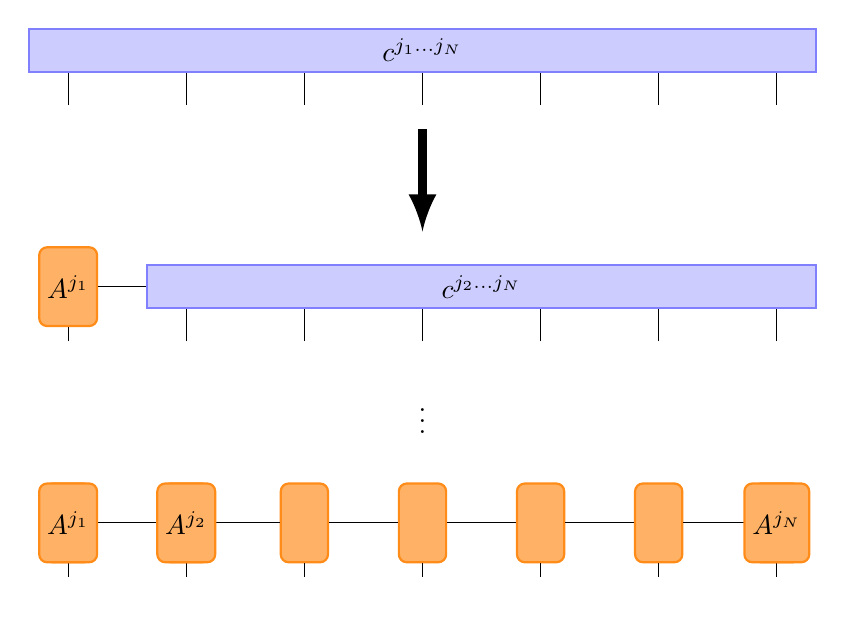
\begin{tikzpicture}[inner sep=1mm]
	\def \numb {7};
	\def \hdist {1.5};
	\def \wid {10};
	\def \wids {8.5};

	\node[tensor, minimum width=\wid cm] (tens1) at (\wid/2 +1, 0) {$c^{j_1 \ldots j_N}$};
	
	\foreach \i in  {1,...,\numb} {
		\node (\i) at (\i*\hdist, -0.8) {};
		\draw[-] (\i) -- (\i |-  tens1.south);	
	};
	
	\draw[->, line width=1.25mm] (\wid/2 +1,-1) -- (\wid/2 +1,-2.3);
	
	\node[tensorl] (blok1) at (1*\hdist, -3) {$A^{j_1}$};
	\node[tensor, minimum width=\wids cm] (tens2) at (\wids/2 +2.5, -3) {$c^{j_2 \ldots j_N}$};
	
	\foreach \i in  {2,...,\numb} {
		\node (\i) at (\i*\hdist, -3.8) {};
		\draw[-] (\i) -- (\i |-  tens2.south);	
	};
	\node (node1) at (1*\hdist, -3.8) {};
	\draw[-] (node1) -- (blok1);
	\draw[-] (tens2) -- (blok1);
	
	\node (dots) at (\wid/2 +1, -4.6) {\vdots};
	
	\foreach \i in  {1,...,\numb} {
		\node[tensorl] (t\i) at (\i*\hdist, -6) {};
		\node (\i) at (\i*\hdist, -6.8) {};
		\draw[-] (t\i) -- (\i);	
	};
	\foreach \i in  {1,...,6} {
		\pgfmathtruncatemacro{\iplusone}{\i + 1};
		\draw[-] (t\i) -- (t\iplusone);	
	};
	
	\node[tensorl] (lab1) at (1*\hdist, -6) {$A^{j_1}$};
	\node[tensorl] (lab2) at (2*\hdist, -6) {$A^{j_2}$};
	\node[tensorl] (labN) at (\numb*\hdist, -6) {$A^{j_N}$};
	
\end{tikzpicture}
	\caption{\textit{Diagrammatic representation of the construction of a left-canonical MPS from an arbitrary quantum state through successive SVD's.}}
	\label{fig:MPSbuild}
\end{figure}
The construction of an MPS is illustrated in figure \ref{fig:MPSbuild}. Thereby, the original state (equation \ref{eq:arbstate}) can be written as a matrix product state in the form \cite{schollwock}
\begin{equation}
	\ket{\psi} = \sum_{j_1, \ldots, j_N} A^{j_1} A^{j_2} \ldots A^{j_{N-1}} A^{j_{N}} \ket{j_1, \ldots, j_N} \; .
	\label{eq:MPS_LC} 
\end{equation}
\\
It is worth examining the properties of this representation. From the dimensions of the components of an SVD, one will notice the dimensions of the matrices $A^{j_n}$ follow a pyramid-like structure $(1 \times d ),(d \times d^2) , \ldots , (d^{N/2 -1} \times d^{N/2}) , (d^{N/2} \times d^{N/2 -1 }), \ldots , (d \times 1)$, where N is taken as even for simplicity. Hence, the matrix dimensions increase exponentially making exact computations practically impossible. However, certain simplifications can be made, which greatly reduces computational time without sacrificing much precision. First, one only needs to keep the non-zero, singular values of the matrices $S$, thus reducing the dimensional factor from $d$ to $r_n$, where $r_n \leq d$ is the Schmidt rank of the n'th decomposition. Secondly, as discussed earlier, only a few terms is needed to accurately describe entanglement across bonds. Therefore, the matrices $S$, $U$ and $V$ can be truncated, by keeping only the $D$ largest singular values, as these contribute the most to the state. Thus, the dimension of the matrices will cap at $D$: $(1 \times d ),(d \times d^2) , \ldots , (d^{n} \times D) , (D \times D), \ldots , ( D \times d^{n}) \ldots  (d \times 1)$, avoiding the otherwise exponential dimensional growth \cite{EntropyScaling}. The amount of singular values needed to be kept in order to produce an accurate approximation of the state is highly dependent of the system. Thus, one often need to perform the same calculation for various values of $D$, in order to gauge how much the matrices can be truncated.


\section{Canonical Forms}
\label{sec:canonical}
The MPS described in equation \ref{eq:MPS_LC} is not unique, as writing 
\begin{equation}
	\tilde{A}^{j_n} = X_{n-1} A^{j_n} X_{n}^{-1}
\end{equation}
describes the same state using different matrices. This gauge freedom allows expressing the MPS in whichever way is most convenient, often resulting in a much lower numerical cost of operations. By choosing a gauge, the MPS is brought into a \textit{canonical form} \cite{Vidal}.

\subsection{Left-canonical matrix product state}
The process of constructing an matrix product state detailed in Section \ref{sec:construct_MPS} brings the MPS in a \textit{left-canonical} form. This implies that all the matrices are left-normalized, such that
\begin{equation}
	\sum_{j_n} A^{j_n \dag} A^{j_n} = I \; .
	\label{eq:LC_ident}
\end{equation}
This is a consequence of the matrix $U$ (from the SVD) fulfilling $U^{\dag}U = I$. Since the matrices $A^{j_n}$ are reshaped from $U$, these properties persists
\begin{align*}
	\delta_{\alpha_n , \alpha_n'} &= \sum_{\alpha_{n-1} j_n} (U^{\dag})_{\alpha_n , (\alpha_{n-1} j_n)} U_{(\alpha_{n-1} j_n), \alpha_n'} \\
	 &= \sum_{\alpha_{n-1} j_n} (A^{j_n \dag})_{\alpha_n , \alpha_{n-1}} A_{\alpha_{n-1}, \alpha_n'}^{j_n} \\
	 &= \sum_{j_n} \left( A^{j_n \dag} A^{j_n} \right)_{\alpha_{n} . \alpha_n'}
\end{align*} 
\begin{figure}[h!]
	\centering
	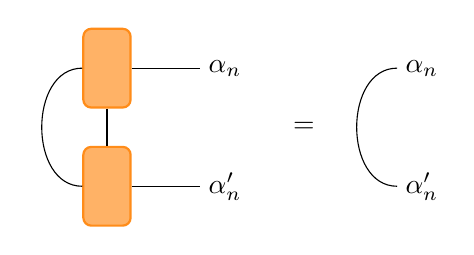
\begin{tikzpicture}[inner sep=1mm]
	\def \vdist {1.5};

	\node[tensorl] (tens1) at (1,0) {};
	\node[tensorl] (tens2) at (1,-\vdist) {}; 
 	
	\node (index1) at (2.5,0) {$\alpha_n$};
	\node (index2) at (2.5,-\vdist) {$\alpha_n '$}; 	
 	
 	\draw[-] (tens1) -- (tens2);
	\draw[-] (tens1) -- (index1);
	\draw[-] (tens2) -- (index2); 	
    \draw[-] (tens1.west) .. controls (0, 0) and (0, -\vdist) .. (tens2.west);
    
    
    \node (eq) at (3.5,-\vdist/2) {$=$};
    
    
 	\node (dummy1) at (5,0) {$\alpha_n$};
 	\node (dummy2) at (5,-\vdist) {$\alpha_n '$};
    
    \draw[-] (dummy1.west) .. controls (4, 0) and (4, -\vdist) .. (dummy2.west);
\end{tikzpicture}
	\caption{\textit{Contraction over the left index (shown as the arc) and the physical index of two left-normalised matrices. The result is $\delta_{\alpha_n , \alpha_n'}$, adding the n'th site to the contraction of all previous sites to the left.}}
	\label{fig:leftNorm}
\end{figure}
Figure \ref{fig:leftNorm} illustrates a contraction of the bonds connecting two left-normalised matrices. As this contraction results in the identity per definition, one can contract left-normalised matrices without any explicit calculation. This is displayed diagrammatically through an arc, which is equivalent to an identity-tensor with two bond indices. 


\subsection{Right-canonical matrix product state}
One could also have built a a right-canonical MPS from eq. \eqref{eq:arbstate}, had one started from other side of the chain. This implies multiplying $U$ and $S$ into the new $\Psi$-matrix, and reshaping $(V^{\dag})_{(\alpha_{n-1} j_n), \alpha_n}$ into matrices $B_{\alpha_{n-1} , \alpha_n}^{j_n}$. Hence, the right-canonical form of the MPS of eq. \eqref{eq:MPS_LC} reads
\begin{equation}
	\ket{\psi} = \sum_{j_1, \ldots, j_N} B^{j_1} B^{j_2} \ldots B^{j_{N-1}} B^{j_{N}} \ket{j_1, \ldots, j_N} \; .
\label{eq:MPS_RC}	 
\end{equation}
In this form all the matrices are right-normalized, whereby 
\begin{equation}
	\sum_{j_n} B^{j_n} B^{j_n \dag} = I \; .
	\label{eq:RC_ident}
\end{equation}
Note how right-normalised matrices are denoted by $B^{j_n}$ opposed to left-normalised matrices, $A^{j_n}$.
Figure \ref{fig:rightNorm} illustrates two right-normalised matrices contracted over their physical index.
\begin{figure}[h!]
	\centering
	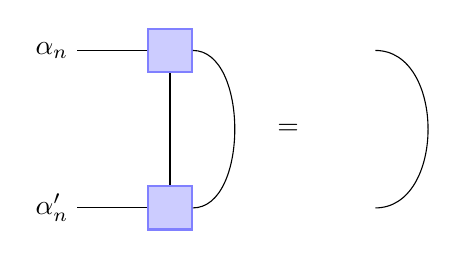
\begin{tikzpicture}[inner sep=1mm]
	\node[tensor] (tens1) at (2.5,0) {};
	\node[tensor] (tens2) at (2.5,-2) {}; 
 	
	\node (index1) at (1,0) {$\alpha_n$};
	\node (index2) at (1,-2) {$\alpha_n '$}; 	
 	
 	\draw[-] (tens1) -- (tens2);
	\draw[-] (tens1) -- (index1);
	\draw[-] (tens2) -- (index2); 	
    \draw[-] (tens1.east) .. controls (3.5, 0) and (3.5, -2) .. (tens2.east);
    
    
    \node (eq) at (4,-1) {$=$};
    
    
 	\node (dummy1) at (5,0) {};
 	\node (dummy2) at (5,-2) {};
    
    \draw[-] (dummy1.east) .. controls (6, 0) and (6, -2) .. (dummy2.east);
\end{tikzpicture}
	\caption{\textit{Contraction over the right index (shown as the arc) and the physical index of two right-normalised matrices.}}
	\label{fig:rightNorm}
\end{figure}


\subsection{Mixed-canonical matrix product state}
In practice one rarely finds use for a purely left- or right-canonical MPS. However, combining the two canonical forms listed above yields the mixed-canonical form. This form results in a natural bi-partitioning of the system into a Schmidt decomposition, and it is especially useful for measuring local properties of the state. CITE\\
Consider the procedure of building an MPS in the left-canonical form, where $c_{j_1 \ldots j_N}$ has been decomposed from the left up until site $n$
\begin{equation}
	c_{j_1 \ldots j_N} = \sum_{\alpha_n} \left( A^{j_1} \ldots  A^{j_n} \right) _{\alpha_n} S_{\alpha_n , \alpha_n} (V^{\dag})_{\alpha_n , (j_{n+1} \ldots j_N)} \; .
\end{equation}
By reshaping $V^{\dag}$  into the matrix $\Psi_{(\alpha_n j_{n+1} \ldots j_{N-1}),j_N}$, one can initiate a successive decomposition from the right, resulting in a set of right-normalized matrices. The final result reads
\begin{equation}
	c_{j_1 \ldots j_N} = A^{j_1} \ldots A^{j_n} S B^{j_{n+1}} \ldots B^{j_N} \; ,
	\label{eq:mixedCanon}
\end{equation}
which is illustrated in figure \ref{fig:mixedCanonical1}.
\begin{figure}[h!]
\centering % <-- add this
\begin{subfigure}[b]{0.45\textwidth}
	\caption{}  	
  	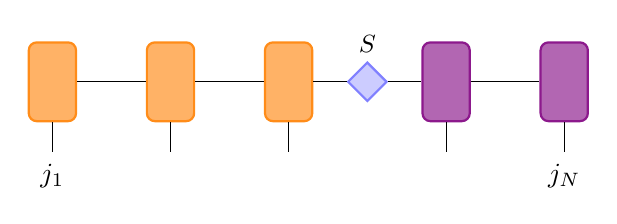
\begin{tikzpicture}[inner sep=1mm]
	\def \hdist {1.5};
	\def \numb {5};
	\def \vleg {1};
	\def \NL {3};

	\foreach \i in  {1,...,\NL} {
		\node[tensorl] (\i) at (\i*\hdist, 0) {};
		\node (index\i) at (\i*\hdist, -\vleg) {};
		\draw[-] (\i) -- (index\i);	
	};
	
	\foreach \i in  {1,...,2} {
		\pgfmathtruncatemacro{\iplusone}{\i + 1};
		\draw[-] (\i) -- (\iplusone);
	};
	
	\foreach \i in  {5,...,6} {
		\node[tensorr] (\i) at (\i*\hdist-\hdist/1.5, 0) {};
		\node (index\i) at (\i*\hdist-\hdist/1.5, -\vleg) {};
		\draw[-] (\i) -- (index\i);	
	};

	\foreach \i in  {5,...,5} {
		\pgfmathtruncatemacro{\iplusone}{\i + 1};
		\draw[-] (\i) -- (\iplusone);
	};
	
	\node[matrix, label={\small $S$}] (S) at (\NL*\hdist+\hdist/1.5,0) {};
	\draw[-] (\NL) -- (S);
	\draw[-] (S) -- (5);
	\node (indexL) at (1*\hdist, -\vleg -0.2) {$j_1$};
	\node (indexR) at (6*\hdist-\hdist/1.5 , -\vleg -0.2) {$j_N$};			
\end{tikzpicture}
	\label{fig:MixedCanonical1}
\end{subfigure}
\hspace{5mm}
\begin{subfigure}[b]{0.45\textwidth}    
	\caption{}  	
  	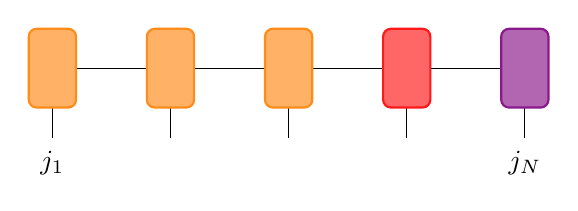
\begin{tikzpicture}[inner sep=1mm]
	\def \hdist {1.5};
	\def \numb {5};
	\def \vleg {1};
	\def \NL {3};

	\foreach \i in  {1,...,\numb} {
		\node[tensor] (\i) at (\i*\hdist, 0) {};
		\node (index\i) at (\i*\hdist, -\vleg) {};
		\draw[-] (\i) -- (index\i);	
	};
	
	\foreach \i in  {1,...,4} {
		\pgfmathtruncatemacro{\iplusone}{\i + 1};
		\draw[-] (\i) -- (\iplusone);
	};
	
	\foreach \i in  {1,...,\NL} {
		\node[tensorl] (\i) at (\i*\hdist, 0) {};
	};
	
	\node[tensorc] (C) at (\numb*\hdist-\hdist, 0) {};
	\node[tensorr] (R) at (\numb*\hdist, 0) {};


	\node (indexL) at (1*\hdist, -\vleg -0.2) {$j_1$};
	\node (indexR) at (\numb*\hdist, -\vleg -0.2) {$j_N$};		
\end{tikzpicture}
	\label{fig:MixedCanonical2}
\end{subfigure}
\caption{\textit{Mixed-canonical form of an MPS. The form \textbf{(i)} directly brings the MPS into the form of a Schmidt decomposition, while the form \textbf{(ii)} is well suited for measuring local properties of the state.}}
\end{figure}
In this form the Schmidt decomposition can be read directly from the form of the MPS by introducing the vectors
\begin{align}
 	\ket{\alpha_n}_A \; &= \; \sum_{j_1 , \ldots , j_n} \left( A^{j_1} \ldots A^{j_n} \right)_{1,\alpha_n} \ket{j_1 , \ldots , j_n}  \label{eq:mixedA} \\
 	\ket{\alpha_n}_B \; &= \; \sum_{j_{n+1} , \ldots , j_N} \left( B^{j_{n+1}} \ldots B^{j_N} \right)_{\alpha_n , 1} \ket{j_{n+1} , \ldots , j_N} \; , \label{eq:mixedB}
\end{align}
whereby the state can be written in the form
\begin{equation}
	\ket{\psi} = \sum_{\alpha_n} S_{\alpha_n , \alpha_n} \ket{\alpha_n}_A \ket{\alpha_n}_B \; .
\end{equation}
In order for this to be a Schmidt decomposition $\sum_{\alpha_n} (S_{\alpha_n , \alpha_n})^2 = 1$, however this condition is fulfilled by default by the SVD. Furthermore, the states $\ket{\alpha_n}_A$ and $\ket{\alpha_n}_B$ have to be orthonormal respectively, which they are by construction.\\
Another useful version of the mixed-canonical form is depicted in figure \ref{fig:MixedCanonical2}, where the matrix $S$ of eq. \eqref{eq:mixedCanon} has been multiplied unto the matrix either to the left or right of it. The result is a central cite, which does not follow any normalisation. This form is advantageous when measuring local properties of a state, as the overlap with itself simplifies to the multiplication of the matrices at the central cite.
 

\subsection{Bringing a matrix product state into canonical form}
Up until now all canonical forms were realised during the construction of the matrix product states. However, any arbitrary MPS can be be brought into a canonical form through a series of SVD's, again exploiting the unitarity or left-/right-normalization of the resulting matrices.\\
Consider a general MPS
\begin{equation}
	\ket{\psi} = \sum_{j_1 , \ldots , j_N} \sum_{\alpha_1 , \ldots } M_{1 , \alpha_1}^{j_1} M_{\alpha_1 , \alpha_2}^{j_2} M_{\alpha_2 , \alpha_3}^{j_3} \ldots \ket{j_1 , \ldots , j_N} \; , 
	\label{eq:generalMPS}
\end{equation}
which has to be brought into a left-canonical form. By grouping the physical and left (row) index of $M_{1 , \alpha_1}^{j_1}$, one can reshape the tensor into a single matrix, $M_{(j_1 , 1) , \alpha_1}$. Applying an SVD yields $M = A S V^{\dag}$, where $A^{\dag} A = I$, such that $A$ is left-normalized as desired. Thus, the left-normalisation of the first tensor of the MPS reads
\begin{align}
\ket{\psi} = & \; \sum_{j_1 , \ldots , j_N} \sum_{\alpha_1 , \ldots } M_{(j_1 , 1) , \alpha_1} M_{\alpha_1 , \alpha_2}^{j_2} M_{\alpha_2 , \alpha_3}^{j_3} \ldots \ket{j_1 , \ldots , j_N} \nonumber \\
= & \; \sum_{j_1 , \ldots , j_N} \sum_{\alpha_1 , \ldots } \sum_{s_1} A_{(j_1 , 1) , s_1} S_{s_1 , s_1} V_{s_1 , \alpha_1}^{\dag} M_{\alpha_1 , \alpha_2}^{j_2} M_{\alpha_2 , \alpha_3}^{j_3} \ldots \ket{j_1 , \ldots , j_N} \nonumber \\
= & \; \sum_{j_1 , \ldots , j_N} \sum_{\alpha_1 , \ldots } \sum_{s_1} A_{1 , s_1}^{j_1} \left( S_{s_1 , s_1} V_{s_1 , \alpha_1}^{\dag} M_{\alpha_1 , \alpha_2}^{j_2} \right) M_{\alpha_2 , \alpha_3}^{j_3} \ldots \ket{j_1 , \ldots , j_N} \nonumber \\
= & \; \sum_{j_1 , \ldots , j_N} \sum_{\alpha_2 , \ldots } \sum_{s_1} A_{1 , s_1}^{j_1} \tilde{M}_{s_1 , \alpha_2}^{j_2} M_{\alpha_2 , \alpha_3}^{j_3} \ldots \ket{j_1 , \ldots , j_N} \; ,
\end{align}
where $\tilde{M}_{s_1 , \alpha_2}^{j_2} = \sum_{\alpha_1} S_{s_1 , s_1} V_{s_1 , \alpha_1}^{\dag} M_{\alpha_1 , \alpha_2}^{j_2}$. This procedure can be iterated through the entire chain, leaving the MPS in the left-canonical form \cite{schollwock}.\\
Likewise, an MPS can be brought into a right-canonical form by grouping the physical index with the right (column) index of $M$ yielding the SVD $M = U S B$, where $B B^{\dag} = I$. Thus, iterating through the chain from the right will produce a right-canonical MPS.

\section{Overlaps and Efficient Contractions}
Great reductions in computational cost can be achieved by contracting the tensor networks in the correct order. Consider the general case of two states $\ket{\psi}$ and $\ket{\phi}$ described by the matrices $M$ and $\tilde{M}$. The overlap between these states reads
\begin{equation}
	\braket{\phi | \psi} = \sum_{j_1 , \ldots , j_N} \tilde{M}^{j_N \dag} \ldots \tilde{M}^{j_1 \dag} M^{j_1} \ldots M^{j_N} \; , 
	\label{eq:overlap}
\end{equation}
which is represented diagrammatically in figure \ref{fig:effCont}.
\begin{figure}[h!]
	\centering
	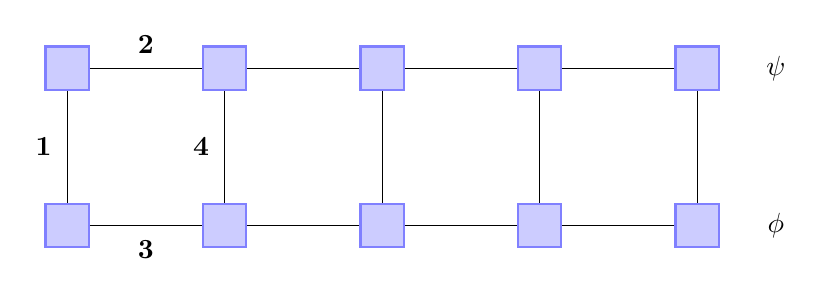
\begin{tikzpicture}[inner sep=1mm]
	\foreach \i in  {1,...,5} {
		\node[tensor] (t\i) at (\i*2-1, 0) {};
		\node[tensor] (b\i) at (\i*2-1, -2) {};
		\draw[-] (t\i) -- (b\i);	
	};
	\foreach \i in  {1,...,4} {
		\pgfmathtruncatemacro{\iplusone}{\i + 1};
		\draw[-] (t\i) -- (t\iplusone);
		\draw[-] (b\i) -- (b\iplusone);
	};
	
	\node (node1) at (0.7, -1) {\textbf{1}};
	\node (node2) at (2, 0.3) {\textbf{2}};
	\node (node3) at (2, -2.3) {\textbf{3}};
	\node (node4) at (2.7, -1) {\textbf{4}};
	
	\node (psi) at (10, 0) {$\ket{\psi}$};
	\node (phi) at (10, -2) {$\bra{\phi}$};
\end{tikzpicture}
	\caption{\textit{Efficient contraction of the overlap between two general states $\ket{\psi}$ and $\ket{\phi}$. By contracting the bonds in the specified order the computational cost is greatly reduced.}}
	\label{fig:effCont}
\end{figure}
The evaluation of the overlap can be drastically sped up by considering the optimal order of contractions, which corresponds to an optimal bracketing of eq. \eqref{eq:overlap}:
\begin{equation}
	\braket{\phi | \psi} = \sum_{j_N} \tilde{M}^{j_N \dag} \left( \ldots \left( \sum_{j_2} \tilde{M}^{j_2 \dag} \left( \sum_{j_1} \tilde{M}^{j_1 \dag} M^{j_1} \right) M^{j_2} \right) \ldots \right) M^{j_N} \; .
	\label{eq:optBrackets}
\end{equation}  
Within the innermost bracket a matrix is formed by multiplying a column and a row vector followed by the summation over the first physical index, $j_1$. In the remaining set of brackets three matrices are multiplied and the corresponding physical index is summed over. However, after the first contraction the complexity of the operation does not increase. Consider the worst case scenario of all the matrices being of dimension $(D \times D)$ with a local Hilbert space of dimension $d$. The total operational cost of the optimal contraction is $\mathrm{O}(N D^3 d)$ compared to otherwise exponential complexity of a random order of contractions \cite{schollwock}. The order of contractions described in eq. \eqref{eq:optBrackets} is illustrated in figure \ref{eq:overlap}.\\
When calculating a norm, $\braket{\psi | \psi}$, the canonical form of the MPS greatly reduces to computational time, as having an either left- or right-canonical MPS implies a norm of 1 without any contractions needed. In the case of a left-canonical for, every matrix product of eq. \eqref{eq:optBrackets} is $I$ due to left-orthogonality. Finally, summing over the final index simply yields 1.


\section{Matrix Product Operators} \label{sec:MPO}
A Matrix Product Operator (MPO) is an operator expressed in the formalism of an MPS. Thus, operators can easily be incorporated as part of the tensor networks, where they are evaluated by contraction over their bonds.\\
Consider a single coefficient of an MPS of the state $\psi$
\begin{equation}
	\braket{j_1 , \ldots , j_N | \psi} = \braket{\boldsymbol{j} | \psi} = M^{j_1} M^{j_2} \ldots M^{j_N} \; . 
\end{equation}
Expressing an operator $\hat{O}$ in the basis of the local states, one can write it in a similar manner
\begin{equation}
	\hat{O} = \sum_{\boldsymbol{j} , \boldsymbol{j'}} \ket{\boldsymbol{j}} \bra{\boldsymbol{j}} \hat{O} \ket{\boldsymbol{j'}} \bra{\boldsymbol{j'}} = \sum_{\boldsymbol{j} , \boldsymbol{j'}} W^{j_1 , j_1 '} W^{j_2 , j_2 '} \ldots W^{j_N , j_N '} \ket{\boldsymbol{j}} \bra{\boldsymbol{j '}} \; ,
	\label{eq:MPOrep}
\end{equation}
where the coefficients are $\bra{\boldsymbol{j}} \hat{O} \ket{\boldsymbol{j'}} = W^{j_1 , j_1 '} W^{j_2 , j_2 '} \ldots W^{j_N , j_N '}$. The matrices $W^{j_n , j_n '}$ are just like the $M$-matrices, except the the representation of the operators needs both an ingoing and an outgoing physical index. This corresponds graphically to having two vertical lines; one corresponding to the ingoing physical state, the other corresponding to the outgoing physical state. A pictorial representation of the operator $\hat{O}$ can be seen in figure \ref{fig:MPOchain}.
\begin{figure}[h!]
	\centering
	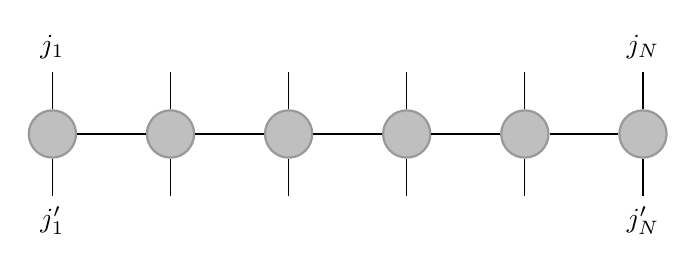
\begin{tikzpicture}[inner sep=1mm]
	\def \numb {6};	
	\def \hdist {1.5};
	
    \foreach \i in {1,...,\numb} {
        \node[operator] (\i) at (\i*\hdist, 0) {};
        \node (t\i) at (\i*\hdist, 0.9) {};
        \node (b\i) at (\i*\hdist, -0.9) {};
        
        \draw[-] (\i) -- (t\i);
        \draw[-] (\i) -- (b\i); 
    };
    
    \foreach \i in {1,...,5} {
        \pgfmathtruncatemacro{\iplusone}{\i + 1};
        \draw[-] (\i) -- (\iplusone);
    };
    
    \node (t1) at (\hdist, 1.1) {$j_1$};
    \node (b1) at (\hdist, -1.1) {$j_1 '$};
    \node (t\numb) at (\numb*\hdist, 1.1) {$j_N$};
    \node (b\numb) at (\numb*\hdist, -1.1) {$j_N '$};
\end{tikzpicture}
	\caption{\textit{An operator $\hat{O}$ expressed in the MPS form (MPO). The resulting matrix product has two vertical lines corresponding to an ingoing and outgoing physical state.}}
	\label{fig:MPOchain}
\end{figure}

\subsection{Applying an MPO to an MPS}
Applying a matrix product operator to a matrix product state is simply a matrix multiplication, where the matching physical indices are summed over:
\begin{align}
	\hat{O} \ket{\psi} &= \sum_{\boldsymbol{j},\boldsymbol{j'}} \left( M^{ j_1 '} M^{j_2 ' } \ldots \right) \left( W^{j_1 ' , j_1} W^{j_2 ' , j_2} \ldots \right) \ket{\boldsymbol{j}} \nonumber \\
	&= \sum_{\boldsymbol{j},\boldsymbol{j'}} \sum_{\boldsymbol{\alpha},\boldsymbol{\beta}} \left( M_{1, \alpha_1}^{ j_1 '} M_{\alpha_1, \alpha_2}^{j_2 '} \ldots \right) \left( W_{1, \beta_1}^{j_1 ' , j_1 } W_{\beta_1, \beta_2}^{j_2 ', j_2 } \ldots \right) \ket{\boldsymbol{j}} \nonumber \\
&= \sum_{\boldsymbol{j},\boldsymbol{j'}} \sum_{\boldsymbol{\alpha},\boldsymbol{\beta}} \left( M_{1, \alpha_1}^{ j_1 '} W_{1, \beta_1}^{j_1 ' , j_1} \right) \left( M_{\alpha_1, \alpha_2}^{j_2 '}  W_{\beta_1, \beta_2}^{j_2 ' , j_2} \right) \ldots \ket{\boldsymbol{j}} \nonumber \\
&= \sum_{\boldsymbol{j}} \sum_{\boldsymbol{\alpha},\boldsymbol{\beta}} N_{(1,1),(\alpha_1 , \beta_1)}^{j_1} N_{(\alpha_1 , \beta_1),(\alpha_2 , \beta_2)}^{j_2} \ldots \ket{\boldsymbol{j}} \nonumber \\
&= \sum_{\boldsymbol{j}} N^{j_1} N^{j_2} \ldots \ket{\boldsymbol{j}} \; = \; \ket{\phi}
\label{eq:optBracketsMPO}
\end{align} 
The result is a new MPS, $\ket{\phi}$, which is described by the matrices $N^{j_n}$ and is illustrated in figure \ref{fig:MPOcont}. These matrices have the dimensions of the product of the dimensions of the original MPS and MPO. Thus, applying an operator leaves the form of the MPS invariant at a cost of increased matrix dimensions.
\begin{figure}[h!]
	\centering
	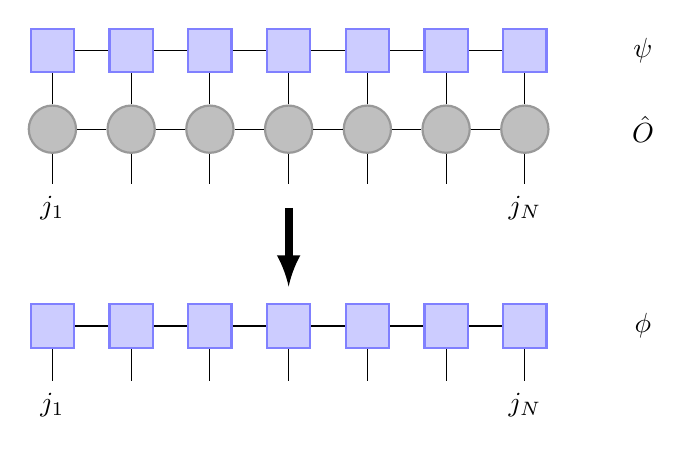
\begin{tikzpicture}[inner sep=1mm]
    \foreach \i in {1,...,7} {
        \node[tensor] (t\i) at (\i, 0) {};
        \node[operator] (o\i) at (\i, -1) {};
        
        \node (b\i) at (\i, -1.8) {};
        
        \draw[-] (t\i) -- (o\i);
        \draw[-] (o\i) -- (b\i); 
    };
    
    \foreach \i in {1,...,6} {
        \pgfmathtruncatemacro{\iplusone}{\i + 1};
        \draw[-] (t\i) -- (t\iplusone);
        \draw[-] (o\i) -- (o\iplusone);
    };
    
    \node (b1) at (1, -2) {$j_1$};
    \node (b7) at (7, -2) {$j_N$};
    
    \node (psi) at (8.5, 0) {$\ket{\psi}$};
    \node (O) at (8.5, -1) {$\hat{O}$};
    
    
    \draw[->, line width=1mm] (4,-2) -- (4,-3);
    
    \foreach \i in {1,...,7} {
        \node[tensor] (t\i) at (\i, -3.5) {};
        
        \node (b\i) at (\i, -4.3) {};
        
        \draw[-] (t\i) -- (b\i); 
    };
    
    \foreach \i in {1,...,6} {
        \pgfmathtruncatemacro{\iplusone}{\i + 1};
        \draw[-] (t\i) -- (t\iplusone);
    };
    
    \node (b1) at (1, -4.5) {$j_1$};
    \node (b7) at (7, -4.5) {$j_N$};
    
    \node (phi) at (8.5, -3.5) {$\ket{\phi}$};
\end{tikzpicture}
	\caption{\textit{Application of an MPO, $\hat{O}$, on an MPS, $\ket{\psi}$. Matching physical indices are contracted resulting in a new MPS, $\ket{\phi}$, with increased matrix dimensions.}}
	\label{fig:MPOcont}
\end{figure}
If the dimension of the MPS is $D$, while the dimension of the MPO is $D_W$, the total computational cost of the operation is $\mathrm{O}(N d^2 D_W ^2 D^2)$.\cite{schollwock, McCulloch}

\section{Correlation Functions and Measurement of Local Properties}
\label{sec:correlationFunctions}
Measuring local properties of a state is achieved by calculating the expectation value of local operators. Consider the local operator $\hat{O}^{[n]}$, where the square brackets denote the site, on which the $\hat{O}$ operates. As $\hat{O}^{[n]}$ is only acts on site $n$, it can be expressed in the basis of said site
\begin{equation}
	\hat{O}^{[n]} = \sum_{j_n , j_n '} O^{j_n , j_n '} \ket{j_n} \bra{j_n '} \; .
	\label{eq:localOperator}
\end{equation}
Applying a local operator to a state implies applying the identity operator on all other sites. The resulting operator, $\hat{O} = \hat{I}^{[1]} \otimes \hat{I}^{[2]} \otimes \ldots \otimes \hat{O}^{[n]} \otimes \ldots \otimes \hat{I}^{[N]}$, can then be expressed as an MPO and readily be applied to a matrix product state. However, the calculation is greatly simplified when considering an MPS in a mixed-canonical form, where all matrices left of site $n$ are left-normalized, while all matrices to the right are right-normalized. In this case, the entire tensor network on either side of site $n$ can be contracted without any calculation. The remaining network needed to be contracted is shown in figure \ref{fig:SingleSiteOperator}, which is simply the sum
\begin{equation}
	\bra{\psi} \hat{O}^{[n]} \ket{\psi} = \sum_{j_n , j_n '} O^{j_n , j_n '} \Tr \left( M^{j_n \dag} M^{j_n '} \right) 
\end{equation}
with the computational cost $\mathrm{O}(D^2 d^2)$ \cite{schollwock}.
\begin{figure}[h!]
\centering % <-- add this
\begin{subfigure}[b]{0.35\textwidth}
  	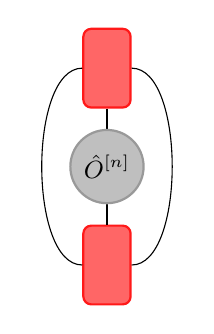
\begin{tikzpicture}[inner sep=1mm]
	\def \vdist {2.5}

	\node[tensorc] (tens1) at (1,0) {};
	\node[tensorc] (tens2) at (1,-\vdist) {}; 
	
	\draw[-] (tens1) -- (tens2);	
	
 	\node[operator] (op) at (1,-\vdist/2) {\small $\hat{O}^{[n]}$};
 	
 
    \draw[-] (tens1.west) .. controls (0, 0) and (0, -\vdist) .. (tens2.west);
    \draw[-] (tens1.east) .. controls (2, 0) and (2, -\vdist) .. (tens2.east);
\end{tikzpicture}
	\caption{}
	\label{fig:SingleSiteOperator}
\end{subfigure}
\begin{subfigure}[b]{0.35\textwidth}    
  	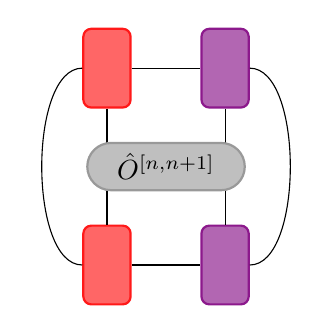
\begin{tikzpicture}[inner sep=1mm]
	\def \vdist {2.5}
	\def \hdist {1.5}
	\def \wid {2}

	\node[tensorc] (tens1) at (1,0) {};
	\node[tensorc] (tens2) at (1,-\vdist) {};
	\node[tensorr] (tens3) at (1 + \hdist,0) {};
	\node[tensorr] (tens4) at (1 + \hdist,-\vdist) {};

	\draw[-] (tens1) -- (tens2);
 	\draw[-] (tens3) -- (tens4);
 	\draw[-] (tens1) -- (tens3);
 	\draw[-] (tens2) -- (tens4);
	 
 	\node[twositeop, minimum width= \wid cm] (op) at (1 + \hdist/2 ,-\vdist/2) { $\hat{O}^{[n, n+1]}$};
 	
 
    \draw[-] (tens1.west) .. controls (0, 0) and (0, -\vdist) .. (tens2.west);
    \draw[-] (tens3.east) .. controls (2+\hdist, 0) and (2+\hdist, -\vdist) .. (tens4.east);
\end{tikzpicture}
	\caption{}
	\label{fig:DoubleSiteOperator}
\end{subfigure}
\caption{\textit{Measurement of local properties of a matrix product state in the mixed-canonical form.}}
\end{figure}
Very similar is the case of multiple-site local operator. However, sites on which the operator act can not be contracted explicitly. Thus, the resulting tensor network will look like the example shown in figure \ref{fig:DoubleSiteOperator}, where a two-site operator is measured.\\

Also correlation functions are calculated efficiently using matrix product states in the mixed-canonical form. Consider the correlation $\bra{\psi} \hat{O}^{[n]} \hat{Q}^{[n+k]} \ket{\psi}$, whose corresponding tensor network is shown in figure \ref{fig:CorrelationFunction}.
\begin{figure}[h!]
	\centering
	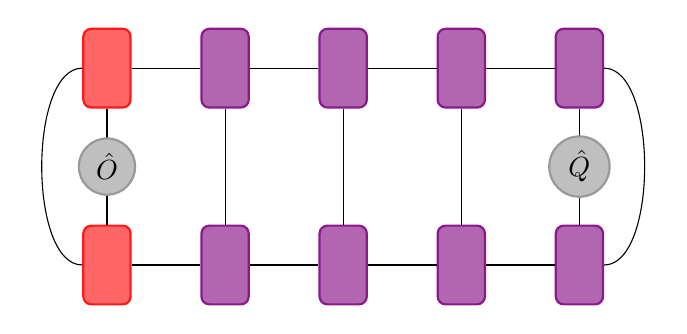
\begin{tikzpicture}[inner sep=1mm]
	\def \vdist {2.5};
	\def \hdist {1.5};
	\def \wid {2};
	\def \numb {5};

	\node[tensorc] (tt1) at (1*\hdist,0) {};
	\node[tensorc] (tb1) at (1*\hdist,-\vdist) {};
	
	 \foreach \i in {2,...,\numb} {
        \node[tensorr] (tt\i) at (\i*\hdist, 0) {};
		\node[tensorr] (tb\i) at (\i*\hdist,-\vdist) {};
           
        \draw[-] (tt\i) -- (tb\i);
    };
    
    \foreach \i in {2,...,4} {
        \pgfmathtruncatemacro{\iplusone}{\i + 1};
        \draw[-] (tt\i) -- (tt\iplusone);
        \draw[-] (tb\i) -- (tb\iplusone);
	};

	\draw[-] (tt1) -- (tb1);
 	\draw[-] (tt1) -- (tt2);
 	\draw[-] (tb1) -- (tb2);
 	 
 	\node[operator] (op1) at (1*\hdist,-\vdist/2) {$\hat{O}$};
	\node[operator] (op2) at (\numb*\hdist,-\vdist/2) { $\hat{Q}$};
  
 
    \draw[-] (tt1.west) .. controls (\hdist-1, 0) and (\hdist-1, -\vdist) .. (tb1.west);
    \draw[-] (tt\numb.east) .. controls (1+\numb*\hdist, 0) and (1+\numb*\hdist, -\vdist) .. (tb\numb.east);
\end{tikzpicture}
	\caption{\textit{Tensor network for the correlation function $\bra{\psi} \hat{O}^{[n]} \hat{Q}^{[n+4]} \ket{\psi}$. The outer parts of the network are implicitly contracted to identities following the mixed-canonical form of the MPS.}}
	\label{fig:CorrelationFunction}
\end{figure}
Again, having brought the MPS unto a mixed-canonical form results in the outer parts of the network being explicitly contracted as identities. However, the otherwise right-normalised tensors between the two operators can not be contracted as identities, as the right-most operator breaks the canonical form. Thus, one has to contract a network of length $k+1$, which is done most efficiently following the optimal bracketing described in eq. \eqref{eq:optBracketsMPO}. The complexity of the entire contraction is of order $O(k D^3 d)$.

\subsection{Correlation length}
Although the MPS formalism excels at describing one dimensional systems, it struggles with describing long ranged correlations, due to how it is constructed.
Consider a general MPS in no particular canonical form, as described in eq. \eqref{eq:generalMPS}. The \textit{transfer operator} is defined as
\begin{equation}
	\hat{E}^{[n]} = \sum_{\alpha_{n-1}, \alpha_{n-1}'} \sum_{\alpha_{n}, \alpha_{n}'} \left( \sum_{j_n} M^{[n] j_n *} \otimes  M^{[n] j_n} \right)_{(\alpha_{n-1} \alpha_{n-1}'),(\alpha_{n}  \alpha_{n}')} \left( \ket{\alpha_{n-1}}\bra{\alpha_{n-1}'} \right) \left( \ket{\alpha_{n}}\bra{\alpha_{n}'} \right) \; ,
\end{equation}   
where the expression in the brackets is the matrix elements of the operator, and $\alpha_n$ are the physical indices of the matrices. The transfer operator is essentially a complete, positive map from operators defined on a block of the lattice of length $n-1$ to a block of length $n$, such that
\begin{equation}
	\{ \ket{\alpha_{n-1}}\bra{\alpha_{n-1}'} \} \to \{ \ket{\alpha_{n}}\bra{\alpha_{n}'} \} \; .
\end{equation}
One important property of the transfer operator, or transfer matrix, is that all eigenvalues $|\lambda_k| \leq 1 $ \cite{schollwock}. \\
Generalizing the transfer operator to contraction with an operator $\hat{O}$ gives
\begin{equation}
	E_{O}^{[n]} = \sum_{j_n , j_n '} O^{j_n , j_n '} M^{[n] j_n *} \otimes  M^{[n] j_n '} \; .
\end{equation}
Using this one can write the correlation function of two general operators on sites $i$ and $j$ as
\begin{align}
	\bra{\psi} \hat{O}^{[i]} \hat{O}^{[j]} \ket{\psi} &= \Tr E^{[1]} \ldots E^{[i-1]} E_{O}^{[i]} E^{[i+1]} \ldots E^{[j-1]} E_{O}^{[j]} E^{[j+1]} \ldots E^{[N]} \nonumber \\
	&= \Tr E_{O}^{[i]} E^{[j-i-1]} E_{O}^{[j]} E^{[L-j+i-1]} \nonumber \\ 
	&= \sum_{l , k} \bra{l} E_{O}^{[i]} \ket{k} \lambda_{k}^{j-i-1} \bra{k} E_{O}^{[j]} \ket{l} \lambda_{l}^{N-j+i-1} \nonumber \\ 
	&= \sum_{k} \bra{1} E_{O}^{[i]} \ket{k} \lambda_{k}^{j-i-1} \bra{k} E_{O}^{[j]} \ket{1} \qquad (\mathrm{for } N \to \infty)
\end{align}
where $\lambda$ is the eigenvalues of the transfer matrix. Since $|\lambda_k| \leq 1 $, only the leading eigenvalue $\lambda_1 = 1$ remains as $N \to \infty$. Defining the distance between two sites as $r = |j - i -1|$ and the correlation decay, or correlation length, as $\xi_k = -1/\ln \lambda_k$, the correlation function can be written as
\begin{equation}
	\frac{\bra{\psi} \hat{O}^{[i]} \hat{O}^{[j]} \ket{\psi}}{\braket{\psi | \psi}} = c_1 + \sum_{k = 2} c_k e^{-r/ \xi_k} \; , \label{eq:corrfunction}
\end{equation}
where $c_k = \bra{1} E_{O}^{[i]} \ket{k} \bra{k} E_{O}^{[j]} \ket{1}$. \cite{schollwock} \\
According to eq. \eqref{eq:corrfunction}, correlation functions are given by a linear combination of exponential functions in the MPS description. As eq. \eqref{eq:corrfunction} was derived without any assumptions regarding neither the MPS nor the operators, the results can be considered general. Thus, any finite-dimensional MPS will only be able to approximate the true correlation of a system.\\
This is the cause of the difficulty of describing the long range correlations, such as the Superfluid single-particle correlations. While single-particle correlations decay exponentially for the Mott-Insulator, it decays following a power-law for Superfluids
\begin{equation}
	\braket{\hat{a}_{i}^{\dag} \hat{a}_{j}} \sim |i - j|^{-K_b /2} \; ,
	\label{eq:superfluidCorrelation}
\end{equation}
where $K_b$ is the Tomonaga-Luttinger parameter \cite{characPhases}. For short distances eq. \eqref{eq:corrfunction} is able to accurately approximate a power-law, however, only the slowest exponential decay will survive, as distances grow larger. Hence, the correlation turns into a pure exponential decay with $\xi = -1/ \ln \lambda$, where $\lambda$ is the largest eigenvalue of $\hat{E}$ contributing to the correlation.\\
To demonstrate the correlation properties of matrix product states, consider figure \ref{fig:DensityMatrices}.
\begin{figure}[h!]
    \centering
    \includegraphics[width=\textwidth]{Figures/DensityMatrices.pdf}
    \caption{\textit{Density matrix of a 50 site system for various fractions of $U/J$. In \textbf{iv} the matrix entries of the 15th row is plotted as a function of distance from the diagonal, $r$. }}
    \label{fig:DensityMatrices}
\end{figure}
The figure depict the density matrix, with entries $\rho_{i,j} = \bra{\psi} \hat{a}_{i}^{\dag} \hat{a}_{j} \ket{\psi}$, of a system of size $N = 50$ with unit occupancy. The ground state $\ket{\psi}$ was found using the DMRG algorithm detailed in Section \ref{sec:DMRG}.
Figures \ref{fig:DensityMatrices}.i and \ref{fig:DensityMatrices}.iii show the density matrix plotted for the Superfluid and the Mott-Insulator limit respectively. In the Superfluid limit, long-range correlations are present, which is seen by large off-diagonal elements. However, since all correlations decay exponentially in the MPS description, the algorithm has difficulty approximating the very long range correlations of the system. This is visualized in figure \ref{fig:DensityMatrices}.iv, where the correlation function is plotted against distance from the diagonal. The Superfluid graph has a hump on it, which is an artifact of the DMRG algorithm. Due to the very long correlation length, the graph should be almost flat except for the rapid drop in the end, which is due to the open boundary conditions.\\
In the Mott-Insulator limit no interaction takes place between sites, and the correlation length is zero. Hence, the correlation matrix contains only diagonal elements of equal magnitude. Figure \ref{fig:DensityMatrices}.iii shows some off-diagonal elements of non-zero magnitude, however, this system is not a pure Mott-Insulator, as $U/J = 12$. Nevertheless, the correlations are well described by only a single exponential function, as seen by the figure.\\
Finally, figure \ref{fig:DensityMatrices}.ii illustrates the density matrix for a system with $U/J = 0.5$, which is primarily as Superfluid. The particles are not completely de-localized, which is noticeable from the well defined diagonal. Plotting the correlation function reveals the best approximation being a power-law, thus confirming the system is indeed a Superfluid. 




\chapter{Tensor Network Algorithms}
Although matrix product states enables analytical treatment of certain classes of quantum states \cite{Baxter1968,Affleck1987}, their real power becomes evident when performing numerical computations. These computations require algorithms, which are capable of exploiting the properties of the matrix product states. The Density-Matrix Renormalization Group (DMRG) was developed as the most powerful numerical method to study one-dimensional quantum lattice systems \cite{White1992,White1993}. Years later the connection between the DMRG method and matrix product states was made, as these two approaches share many features \cite{Ostlund1995, Dukelsky1998}. Formulating the DMRG method in the MPS language made several extensions to the algorithm possible, which would otherwise have been very difficult to express within the DMRG framework \cite{schollwock}. Among these extensions one finds the tDMRG algorithm, which borrows elements from DMRG in order to perform time-evolution of a matrix product state.\\
This chapter covers variational ground state search through the DMRG method and time-evolution of matrix product states through the tDMRG algorithm.


\section{Variational Ground State Search}
For large systems exact diagonalization of the Hamiltonian is impossible, whereby one must resort to variational methods in order to find ground states. This involves finding the MPS, $\ket{\psi}$, which minimizes
\begin{equation}
	E = \frac{\bra{\psi} \hat{H} \ket{\psi}}{\braket{\psi | \psi}} \; .
\end{equation}
The most efficient way to do this, is to express the Hamiltonian as an MPO as described in eq. \eqref{eq:MPOrep}, whereby it easily can be applied to an MPS. While this may seem difficult at first, it can actually be done without any lengthy calculations. An example is given in Appendix \ref{chap:buildMPO}, where the Bose-Hubbard Hamiltonian is formulated as tensors.

\subsection{Efficient Application of a Hamiltonian to an MPS}
In section \ref{sec:MPO} it was explained how to apply an MPO to an MPS, and it was shown how to efficiently evaluate local operators. However, since $\hat{H} \ket{\psi}$ must be evaluated many times during variational methods, one must find even more efficient way of applying the operator.\\
Consider an MPS in a mixed-canonical form
\begin{align}
	\ket{\psi} &= \sum_{\boldsymbol{j}} A^{j_1} \ldots A^{j_{n-1}} \Psi^{j_n} B^{j_{n+1}} \ldots B^{j_{N}} \ket{\boldsymbol{j}} \nonumber \\
	&= \sum_{\alpha_{n-1} , \alpha_{n}} \ket{\alpha_{n-1}}_A \Psi_{\alpha_{n-1} , \alpha_{n}}^{j_n}  \ket{\alpha_{n}}_B \; ,
	\label{eq:MPSmixedsingle}
\end{align}
where $\Psi^{j_n}$ is the central site, and $\ket{\alpha_{n-1}}_A$ and $\ket{\alpha_{n}}_B$ are block states introduced in eq. \eqref{eq:mixedA} and \eqref{eq:mixedB} respectively.
Huge reductions in computational cost of the variational search can be found by re-using as many calculations as possible. In the basis $\{ \ket{\alpha_{n-1} } \; , \; \ket{ j_n } \; , \; \ket{\alpha_{n} } \}$ the individual matrix elements of the Hamiltonian can be expressed as
\begin{equation*}
	\bra{\alpha_{n-1} j_n \alpha_{n}} \hat{H} \ket{\alpha_{n-1} ' j_n ' \alpha_{n} '} = \sum_{\boldsymbol{j} , \boldsymbol{j'}}  W^{j_1 , j_1 '} \ldots W^{j_N , j_N '}  \braket{\alpha_{n-1} j_n \alpha_{n} | \boldsymbol{j}} \braket{\boldsymbol{j'} | \alpha_{n-1} ' j_n ' \alpha_{n} '} \; . 
\end{equation*}
Since the basis of local states $\{ \ket{\boldsymbol{j}} \}$ shares a state with the basis $\{ \ket{\alpha_{n-1} } \; , \; \ket{ j_n } \; , \; \ket{\alpha_{n} } \}$, the above expression can be re-written using $\sum_{\boldsymbol{j}} \braket{j_n | \boldsymbol{j}} = \sum_{\boldsymbol{j *}} \ket{ \boldsymbol{j *}}$, where "$\boldsymbol{*}$" means "excluding $j_n$". Thus,
\begin{align}
&	\bra{\alpha_{n-1} j_n \alpha_{n}} \hat{H} \ket{\alpha_{n-1} ' j_n ' \alpha_{n} '} = \nonumber \\
 &= \sum_{\boldsymbol{j *} , \boldsymbol{j' * }}  W^{j_1 , j_1 '} \ldots W^{j_n , j_n '} \ldots W^{j_N , j_N '} \nonumber \\
	& \qquad \times \braket{\alpha_{n-1} | j_1 \ldots j_{n-1}} \braket{\alpha_{n} | j_{n+1} \ldots j_{N}} \braket{j_1 ' \ldots j_{n-1} ' | \alpha_{n-1} '} \braket{j_{n+1} ' \ldots j_{N} ' | \alpha_{n} '} \nonumber \\
	&= \sum_{\boldsymbol{j *} , \boldsymbol{j' * }}  W^{j_1 , j_1 '} \ldots W^{j_n , j_n '} \ldots W^{j_N , j_N '} \nonumber \\
	& \qquad \times \left( A^{j_1} \ldots A^{j_{n-1}} \right)_{1 , \alpha_{n-1}}^{*} \left( B^{j_{n+1}} \ldots B^{j_{N}} \right)_{ \alpha_{n} , 1}^{*} \left( A^{j_1 '} \ldots A^{j_{n-1} '} \right)_{1 , \alpha_{n-1} '} \left( B^{j_{n+1} '} \ldots B^{j_{N} '} \right)_{ \alpha_{n} ' , 1} \nonumber \\
	&= \sum_{\alpha_n , \beta_n , \alpha_n '}
	\left( \sum_{j_1 , j_1 '} A_{1 , \alpha_1}^{j_1 *} W_{1, \beta_1}^{j_1 , j_1 '} A_{1 , \alpha_1 '}^{j_1 '} \right)
	\left( \sum_{j_2 , j_2 '} A_{\alpha_1 , \alpha_2}^{j_2 *} W_{\beta_1, \beta_2}^{j_2 , j_2 '} A_{\alpha_1 ' , \alpha_2 '}^{j_2 '} \right)
	\ldots W_{\beta_{n_1}, \beta_n}^{j_n , j_n '} \nonumber \\
	& \qquad \times \left( \sum_{j_{n+1} , j_{n+1} '} B_{\alpha_n , \alpha_{n+1}}^{j_{n+1} *} W_{\beta_n, \beta_{n+1}}^{j_{n+1} , j_{n+1} '} B_{\alpha_n ', \alpha_{n+1} '}^{j_{n+1} '} \right)
	\left( \sum_{j_{N} , j_{N} '} B_{\alpha_{N-1} , 1}^{j_{N} *} W_{\beta_{N-1}, 1}^{j_{N} , j_{N} '} B_{\alpha_{N-1}' , 1 }^{j_{N} '} \right)  \; .
\end{align}  
While this expression may seem terrible complicated due to all the indices, it is actually rather easy to understand. First, the matrix element is written excluding the local basis state $\ket{j_n}$. Next, the Hamilton MPO is projected into the block states of A, $\ket{\alpha_{n-1}}_A$, and B, $\ket{\alpha_{n}}_B$. Finally, the matrices are grouped according to their expansion in the local basis. Working with the above expression appears cumbersome, but it is merely a decoupling of the system into three distinct parts, which can be seen in figure \ref{fig:singleElemHamil}.
\begin{figure}[h!]
	\centering
	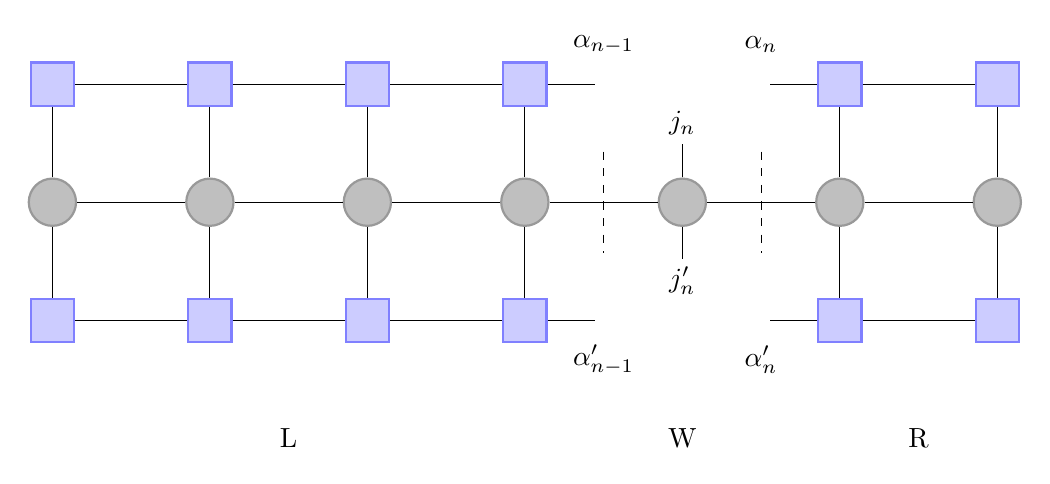
\begin{tikzpicture}[inner sep=1mm]
    \foreach \i in {1,...,4} {
        \node[tensor] (tt\i) at (2* \i -1, 0) {};
        \node[operator] (o\i) at (2* \i -1, -1.5) {};
        \node[tensor] (tb\i) at (2* \i -1, -3) {};
        
        
        \draw[-] (tt\i) -- (o\i);
        \draw[-] (o\i) -- (tb\i);
    };
    \foreach \i in {6,...,7} {
        \node[tensor] (tt\i) at (2* \i -1, 0) {};
        \node[operator] (o\i) at (2* \i -1, -1.5) {};
        \node[tensor] (tb\i) at (2* \i -1, -3) {};
        
        
        \draw[-] (tt\i) -- (o\i);
        \draw[-] (o\i) -- (tb\i);
    };
        \foreach \i in {1,...,3} {
        \pgfmathtruncatemacro{\iplusone}{\i + 1};
        \draw[-] (tt\i) -- (tt\iplusone);
        \draw[-] (tb\i) -- (tb\iplusone);
        \draw[-] (o\i) -- (o\iplusone);
    };
    \draw[-] (tt6) -- (tt7);
    \draw[-] (tb6) -- (tb7);
    \draw[-] (o6) -- (o7);
    
    
       
	\node[operator] (o5) at (2* 5 -1, -1.5) {};    
    
    \node (a1) at (8,0.5) {$\alpha_{n-1}$};
    \node (a2) at (10,0.5) {$\alpha_{n}$};
    \node (a1p) at (8,-3.5) {$\alpha_{n-1} '$};
    \node (a2p) at (10,-3.5) {$\alpha_{n} '$};
    \node (j) at (9,-0.5) {$j_n$};
    \node (jp) at (9,-2.5) {$j_n '$};
    
    \node (a1d) at (8,0) {};
    \node (a2d) at (10,0) {};
    \node (a1pd) at (8,-3) {};
    \node (a2pd) at (10,-3) {};
    
    \draw[-] (tt4) -- (a1d);
    \draw[-] (tt6) -- (a2d);
    \draw[-] (tb4) -- (a1pd);
    \draw[-] (tb6) -- (a2pd);
    \draw[-] (o5) -- (j);
    \draw[-] (o5) -- (jp);
    \draw[-] (o5) -- (o4);
    \draw[-] (o5) -- (o6);
    
    \node (d1) at (8,-0.75) {};
    \node (d2) at (8,-2.25) {};
   	\draw[dashed] (d1) -- (d2);
   	\node (d3) at (10,-0.75) {};
    \node (d4) at (10,-2.25) {};
   	\draw[dashed] (d3) -- (d4);
   	
   	
   	\node (L) at (4,-4.5) {L};
   	\node (W) at (9,-4.5) {W};
   	\node (R) at (12,-4.5) {R};
\end{tikzpicture}
	\caption{\textit{Representation of the matrix element $\bra{\alpha_{n-1} j_n \alpha_{n}} \hat{H} \ket{\alpha_{n-1} ' j_n ' \alpha_{n} '}$ as an tensor network. Expressing the matrix element in this form decouples the network in three parts: The matrices of the MPO, $W^{[n]}$, connecting the physical sites of the matrix element, and contracted parts L and R consisting of the rest of the MPO and the left- and right-normalised part of the MPS respectively.}}
	\label{fig:singleElemHamil}
\end{figure}
Since both the left and right side of the network is connected, one can contract these parts into two separate tensors $L$ and $R$ called "environments":
\begin{align}
	L_{\alpha_{n-1}, \beta_{n-1} , \alpha_{n-1} '} &= \sum_{ \substack{ \{ \alpha_i \beta_i \alpha_i ' \} \\ i < n-1}} \left( \sum_{j_1 , j_1 '} A_{1 , \alpha_1}^{j_1 *} W_{1, \beta_1}^{j_1 , j_1 '} A_{1 , \alpha_1 '}^{j_1 '} \right) \ldots \left( \sum_{j_{n-1} , j_{n-1} '} A_{\alpha_{n-2} , \alpha_{n-1}}^{j_{n-1} *} W_{\beta_{n-2}, \beta_{n-1}}^{j_{n-1} , j_{n-1} '} A_{\alpha_{n-2} ' , \alpha_{n-1} '}^{j_{n-1} '} \right) \label{eq:Ltensor} \\
	R_{\alpha_{n} ,\beta_{n} , \alpha_{n} '} &= \sum_{ \substack{ \{ \alpha_i \beta_i \alpha_i ' \} \\ i > n}} \left( \sum_{j_{n+1} , j_{n+1} '} B_{\alpha_n , \alpha_{n+1}}^{j_{n+1} *} W_{\beta_n, \beta_{n+1}}^{j_{n+1} , j_{n+1} '} B_{\alpha_n ', \alpha_{n+1} '}^{j_{n+1} '} \right) \left( \sum_{j_{N} , j_{N} '} B_{\alpha_{N-1} , 1}^{j_{N} *} W_{\beta_{N-1}, 1}^{j_{N} , j_{N} '} B_{\alpha_{N-1}' , 1 }^{j_{N} '} \right) \label{eq:Rtensor}
\end{align}
From these contractions, the obvious tripartite structure of the Hamiltonian matrix element, as seen in figure \ref{fig:singleElemHamil}, can be written in a compact way
\begin{equation}
	\bra{\alpha_{n-1} j_n \alpha_{n}} \hat{H} \ket{\alpha_{n-1} ' j_n ' \alpha_{n} '} = \sum_{\beta_{n-1} , \beta_{n}} L_{\alpha_{n-1}, \beta_{n-1} , \alpha_{n-1} '} \; W_{\beta_{n_1}, \beta_n}^{j_n , j_n '} \; R_{\alpha_{n} ,\beta_{n} , \alpha_{n} '} \; .
\end{equation}
Finally, applying this parametrization of the Hamiltonian to the MPS of eq. \eqref{eq:MPSmixedsingle} yields \cite{schollwock}
\begin{equation}
	\hat{H} \ket{\psi} = \sum_{\beta_{n-1} , \beta_{n}} \sum_{\alpha_{n-1}' , j_n ', \alpha_{n}'} L_{\alpha_{n-1}, \beta_{n-1} , \alpha_{n-1} '} \; W_{\beta_{n_1}, \beta_n}^{j_n , j_n '} \; R_{\alpha_{n} ,\beta_{n} , \alpha_{n} '} \; \Psi_{\alpha_{n-1} ' , \alpha_{n} '}^{j_n '} \ket{\alpha_{n-1}}_A \ket{j_n} \ket{\alpha_{n}}_B \; .
	\label{eq:HPsi}
\end{equation}
As mentioned earlier, evaluating $\hat{H} \ket{\psi}$ must be done many times during a variational search of the ground state, hence this operation must be executed as fast as possible. Examining eq. \eqref{eq:HPsi} one will notice, that while the boundaries of $L$ and $R$ will change depending on which site is being optimized, the bulk of the two tensors remain constant through a lot of the calculations. Instead of calculating $L$ and $R$ from eq. \eqref{eq:Ltensor} and \eqref{eq:Rtensor} for every evaluation of eq. \eqref{eq:HPsi}, one can iteratively build them, since they only change by one column of the network at a time. Thus, a large number of computations can be reused.\\
Consider the construction of the tensor $L^{[i]}$. This can be built iteratively from the left by contracting the previous left-tensor $L^{[i-1]}$ with the i'th column of the network consisting of $A^{[i]}$, $W^{[i]}$ and $A^{[i] \dag}$
\begin{equation}
	L_{\alpha_i , \beta_i , \alpha_i '}^{[i]} = \sum_{\substack{ j_i , j_i ' \\ \alpha_{i-1} , \beta_{i-1} , \alpha_{i-1} '}} W_{\beta_{i-1} , \beta_i}^{[i] j_i , j_i '} \left( A^{[i] j_i \dag} \right)_{\alpha_i , \alpha_{i-1}} L_{\alpha_{i-1} , \beta_{i-1} , \alpha_{i-1} '}^{[i-1]} A_{\alpha_{i-1} ' , \alpha_i '}^{[i] j_i '} \; .
\end{equation}
This iterative update of $L^{[i]}$ can be seen illustrated in figure \ref{fig:buildLTensor}. The square-bracket notation has been re-introduced to keep track of the tensors relation to the physical sites. In order to remain consistent with notation, the dummy scalars $L_{\alpha_0 , \beta_0 , \alpha_0 '}^{[0]}  = 1  = \alpha_0 , \beta_0 , \alpha_0 '$ has been introduced.\\
\begin{figure}[h!]
	\centering
	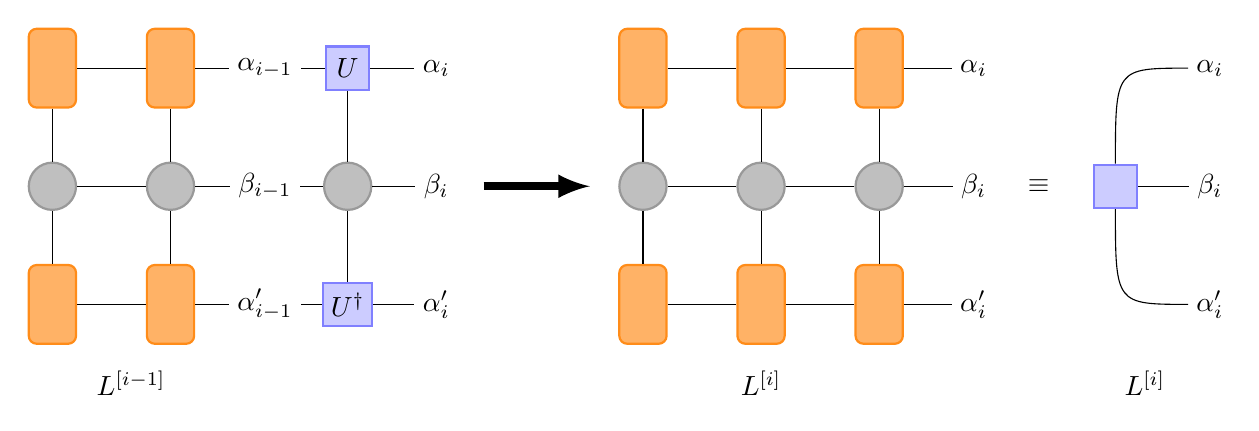
\begin{tikzpicture}[inner sep=1mm]
	\def \numb {2};
	\def \hdist {1.5};
	\def \offset {6};

    \foreach \i in {1,...,\numb} {
        \node[tensorl] (tt\i) at (\i*\hdist, 0) {};
        \node[operator] (o\i) at (\i*\hdist, -1.5) {};
        \node[tensorl] (tb\i) at (\i*\hdist, -3) {};  
        
        \draw[-] (tt\i) -- (o\i);
        \draw[-] (o\i) -- (tb\i);
    };
    \foreach \i in {1,...,1} {
        \pgfmathtruncatemacro{\iplusone}{\i + 1};
        \draw[-] (tt\i) -- (tt\iplusone);
        \draw[-] (tb\i) -- (tb\iplusone);
        \draw[-] (o\i) -- (o\iplusone);
    };
    \foreach \i in {\offset,...,8} {
        \node[tensorl] (tt\i) at (\i*\hdist, 0) {};
        \node[operator] (o\i) at (\i*\hdist, -1.5) {};
        \node[tensorl] (tb\i) at (\i*\hdist, -3) {};  
        
        \draw[-] (tt\i) -- (o\i);
        \draw[-] (o\i) -- (tb\i);
    };
    \foreach \i in {\offset,...,7} {
        \pgfmathtruncatemacro{\iplusone}{\i + 1};
        \draw[-] (tt\i) -- (tt\iplusone);
        \draw[-] (tb\i) -- (tb\iplusone);
        \draw[-] (o\i) -- (o\iplusone);
    };
    
    \node[tensor] (tt) at (\numb*\hdist+1.5*\hdist, 0) {$U$};
    \node[operator] (o) at (\numb*\hdist+1.5*\hdist, -1.5) {};
    \node[tensor] (tb) at (\numb*\hdist+1.5*\hdist, -3) {$U^{\dag}$};

	\draw[-] (tt) -- (o);
	\draw[-] (tb) -- (o);
    
    \node (at1) at (\numb*\hdist+0.8*\hdist, 0) {$\alpha_{i-1}$};
    \node (at2) at (\numb*\hdist+2.25*\hdist, 0) {$\alpha_{i}$};
    \node (ab1) at (\numb*\hdist+0.8*\hdist, -3) {$\alpha_{i-1} '$};
    \node (ab2) at (\numb*\hdist+2.25*\hdist, -3) {$\alpha_{i} '$};
    \node (b1) at (\numb*\hdist+0.8*\hdist, -1.5) {$\beta_{i-1}$};
    \node (b2) at (\numb*\hdist+2.25*\hdist, -1.5) {$\beta_{i}$};
    
    \draw[-] (tt\numb) -- (at1);
    \draw[-] (tb\numb) -- (ab1);
    \draw[-] (o\numb) -- (b1);
    \draw[-] (tt) -- (at1);
    \draw[-] (tb) -- (ab1);
    \draw[-] (o) -- (b1);
    \draw[-] (tt) -- (at2);
    \draw[-] (tb) -- (ab2);
    \draw[-] (o) -- (b2);
    
    
    \draw[->, line width=1mm] (\numb*\hdist+2.65*\hdist,-1.5) -- (\numb*\hdist+3.55*\hdist,-1.5);
    
    \node (at3) at (\offset*\hdist+\numb*\hdist+0.8*\hdist, 0) {$\alpha_{i}$};
    \node (ab3) at (\offset*\hdist+\numb*\hdist+0.8*\hdist, -3) {$\alpha_{i} '$};
    \node (b3) at (\offset*\hdist+\numb*\hdist+0.8*\hdist, -1.5) {$\beta_{i}$};
    \draw[-] (tt8) -- (at3);
    \draw[-] (tb8) -- (ab3);
    \draw[-] (o8) -- (b3);
    
    \node (L1) at (2.5,-4) {$L^{[i-1]}$};
    \node (L2) at (\offset*\hdist+\hdist,-4) {$L^{[i]}$};

    
    \node (eq) at (\offset*\hdist+\numb*\hdist+1.35*\hdist,-1.5) {$\equiv$};
    

    \node (dummy1) at (\offset*\hdist+\numb*\hdist+2.8*\hdist,0) {$\alpha_{i}$};
 	\node (dummy2) at (\offset*\hdist+\numb*\hdist+2.8*\hdist,-3) {$\alpha_{i} '$};
 	\node (dummy3) at (\offset*\hdist+\numb*\hdist+2.8*\hdist,-1.5) {$\beta_{i}$};
	\node[tensor] (mat) at (\offset*\hdist+\numb*\hdist+2*\hdist , -1.5) {};    
    
    \draw[-] (dummy1.west) .. controls (\offset*\hdist+\numb*\hdist+2*\hdist, 0) .. (mat.north);
    \draw[-] (dummy2.west) .. controls (\offset*\hdist+\numb*\hdist+2*\hdist, -3) .. (mat.south);
	\draw[-] (mat) -- (dummy3);   
	
	
	\node (L3) at (\offset*\hdist+\numb*\hdist+2.25*\hdist,-4) {$L^{[i]}$}; 
\end{tikzpicture}
	\caption{\textit{Iterative update from $L^{[i-1]}$ to $L^{[i]}$. This is done through a contraction of $L^{[i-1]}$ with $A^{[i]}$, $W^{[i]}$ and $A^{[i] \dag}$. The result is a tensor with three horizontal legs.}}
	\label{fig:buildLTensor}
\end{figure}
It is important to store every iteration of $L^{[i]}$, since $L$ will grow and shrink constantly throughout the variational search of the ground state, whereby every iteration of $L^{[i]}$ will be used multiple times.
The same applies when building the right environment, $R$. Here one starts from the right and moves left when iteratively contracting the tensor. By applying optimal bracketing, the computational cost of updating the environments scales as $\mathrm{O}(d D^3 D_W)$.
  

\subsection{Iterative Ground State Search and the DMRG Algorithm} \label{sec:DMRG}
In order to find the ground state of the system on can introduce a Lagrangian multiplier, $\lambda$, and extremize
\begin{equation}
	\bra{\psi} \hat{H} \ket{\psi} - \lambda \braket{\psi | \psi} \; ,
	\label{eq:lagrange}
\end{equation}
whereby the desired ground state, $\ket{\psi}$, and ground state energy, $\lambda^0$, will be reached.\\
Trying to optimize an entire MPS at once is a highly non-linear problem involving an extremely large number of variables. However, the problem can be linearised by only considering the variables of a single tensor (site) at a time, while keeping the rest of the MPS constant. By varying just a single tensor at a time, one will continuously find states lower in energy, until convergence is reached. However, this procedure is very prone to getting stuck in a local extrema. To circumvent this, one can consider two sites at a time and optimize with regards to a two-site tensor, created by momentarily merging the two sites \cite{WhiteDMRG}.\\
Consider the variation of the tensors $M^{[n]}$ and $M^{[n+1]}$. Expressing the minimization problem of eq. \eqref{eq:lagrange} in terms of the left and right environments (as done in eq. \eqref{eq:HPsi}) yields
\begin{align}
	\bra{\psi} \hat{H} \ket{\psi} &= \sum_{\substack{j_n , j_n ' \\ j_{n+1} , j_{n+1} '}} \sum_{\alpha_{n-1} ' , \alpha_n ', \alpha_{n+1} '} \sum_{\alpha_{n-1} , \alpha_n , \alpha_{n+1}} \sum_{\beta_{n-1} , \beta_n , \beta_{n+1}} L_{\alpha_{n-1}, \beta_{n-1} , \alpha_{n-1} '}^{[n-1]} \; W_{\beta_{n_1}, \beta_n}^{[n] j_n , j_n '} \; W_{\beta_{n}, \beta_{n+1}}^{[n+1] j_{n+1} , j_{n+1} '} \nonumber \\
	& \qquad \times R_{\alpha_{n+1} ,\beta_{n+1} , \alpha_{n+1} '}^{[n+2]} \; M_{\alpha_{n-1} , \alpha_{n}}^{[n] j_n } \; M_{\alpha_{n-1} ' , \alpha_{n} '}^{[n] j_n ' *} \; M_{\alpha_{n} , \alpha_{n+1}}^{[n+1] j_{n+1} } \; M_{\alpha_{n} ' , \alpha_{n+1} '}^{[n+1] j_{n+1} ' *}  \label{eq:twositeHamil}\\
	\braket{\psi | \psi} &= \sum_{j_n , j_{n+1} } \sum_{\substack{\alpha_{n-1} ' \\ \alpha_n ', \alpha_{n+1} '}} \sum_{\substack{\alpha_{n-1} , \alpha_n \\ \alpha_{n+1}}} \Psi_{\alpha_{n-1},\alpha_{n-1}'}^{A} \; M_{\alpha_{n-1} , \alpha_{n}}^{[n] j_n } \; M_{\alpha_{n-1} ' , \alpha_{n} '}^{[n] j_n ' *} \; M_{\alpha_{n} , \alpha_{n+1}}^{[n+1] j_{n+1} } \; M_{\alpha_{n} ' , \alpha_{n+1} '}^{[n+1] j_{n+1} ' *} \; \Psi_{\alpha_{n+1},\alpha_{n+1}'}^{B} \; , \label{eq:twositeOverlap}
\end{align}
where the Hamiltonian from eq. \eqref{eq:HPsi} has been re-ordered to accommodate examining two sites, $n$ and $n+1$, at a time, and 
\begin{align}
\Psi_{\alpha_{n-1},\alpha_{n-1}'}^{A} &= \sum_{j_1 , \ldots , j_{n-1}} \left( M^{j_{n-1} \dag} \ldots M^{j_{1} \dag} M^{j_1} \ldots M^{j_{n-1}} \right) _{\alpha_{n-1} , \alpha_{n-1} '} \label{eq:psiA} \\
\Psi_{\alpha_{n+1},\alpha_{n+1}'}^{B} &= \sum_{j_{n+2} , \ldots , j_{N}} \left( M^{j_{n+2} } \ldots M^{j_{N} } M^{j_N \dag} \ldots M^{j_{n+2} \dag} \right) _{\alpha_{n+1} ', \alpha_{n+1} } \; .
\end{align}
Further simplifications can be made for mixed-canonical forms, if sites $1$ through $n-1$ are left-normalized, and sites $n+2$ through $N$ are right-normalized, whereby
\begin{equation}
	\Psi_{\alpha_{n-1},\alpha_{n-1}'}^{A} = \delta_{\alpha_{n-1},\alpha_{n-1}'} \qquad , \qquad \Psi_{\alpha_{n+1},\alpha_{n+1}'}^{B} = \delta_{\alpha_{n+1},\alpha_{n+1}'} \; .
\end{equation}
Finding the extremum of eq. \eqref{eq:lagrange} with respect to $M_{\alpha_{n-1} ' , \alpha_{n} '}^{[n] j_n ' *} \; M_{\alpha_{n} ' , \alpha_{n+1} '}^{[n+1] j_{n+1} ' *}$ is done through the following sequence:

\subsubsection{Two-site update for iterative ground state search}
\begin{enumerate}
\item
\textbf{Merge:} Contract the two matrices $M^{[n]}$ and $M^{[n+1]}$ over the bond $\alpha_{n}$ creating a two-site tensor
\begin{equation}
\Theta_{\alpha_{n-1} , \alpha_{n+1}}^{j_n , j_{n+1}} = \sum_{\alpha_n} M_{\alpha_{n-1} , \alpha_{n}}^{[n] j_n } \;  M_{\alpha_{n} , \alpha_{n+1}}^{[n+1] j_{n+1} } 
\end{equation}

\item
\textbf{Solve eigenproblem:} This yields an eigenvalue problem, which can be seen by reshaping
\begin{align}
	H_{( \alpha_{n-1}  j_n  j_{n+1}, \alpha_{n+1}),(\alpha_{n-1}'  j_n '  j_{n+1}', \alpha_{n+1}')} &= \nonumber \\
	= \; \sum_{\substack{\beta_{n-1} , \beta_n \\ \beta_{n+1}}} L_{\alpha_{n-1}, \beta_{n-1} , \alpha_{n-1} '}^{[n-1]} & \; W_{\beta_{n_1}, \beta_n}^{[n] j_n , j_n '} \; W_{\beta_{n}, \beta_{n+1}}^{[n+1] j_{n+1} , j_{n+1} '}\;  R_{\alpha_{n+1} ,\beta_{n+1} , \alpha_{n+1} '}^{[n+2]} \\
	v_{ \alpha_{n-1} j_n j_{n+1} \alpha_{n+1}} &= \; \Theta_{\alpha_{n-1} , \alpha_{n+1}}^{j_n , j_{n+1}}
\end{align}
such that
\begin{equation}
	H v - \lambda v = 0 \; .
	\label{eq:eigprob}
\end{equation}
Solving this for the lowest eigenvalue $\lambda_0$ yields $v_{ \alpha_{n-1} j_n j_{n+1} \alpha_{n+1}}^0$, which can be reshaped back to the now optimized two-site tensor, $\tilde{\Theta}_{\alpha_{n-1} , \alpha_{n+1}}^{j_n , j_{n+1}}$.

\item
\textbf{Unmerge:} Reshape the updated $\tilde{\Theta}_{\alpha_{n-1} , \alpha_{n+1}}^{j_n , j_{n+1}}$ to a matrix and perform an SVD yielding
\begin{equation}
	\tilde{\Theta}_{(j_n \alpha_{n-1} ) ,(j_{n+1}  \alpha_{n+1} )} = \sum_{\alpha_n} U_{\alpha_{n-1} , \alpha_{n}}^{j_n} S_{\alpha_n , \alpha_n} (V^{\dag})_{\alpha_{n} , \alpha_{n+1}}^{j_{n+1}} \; .
\end{equation}
This causes the bond dimension to increase $D \rightarrow d D$, which must be truncated by keeping only the $D$ largest singular values of $S$. 

\item
\textbf{Update environments:} The last step depends on which direction, one is iterating trough the chain. Here, the left- and right-normalization of $U$ and $V^{\dag}$ is used to update the environments.\\
\textit{Going right}: Update the left environment
\begin{equation}
	\tilde{L}_{\alpha_{n}, \beta_{n} , \alpha_{n} '}^{[n]} = \sum_{\substack{ j_{n} , j_{n} ' \\ \alpha_{n-1} , \beta_{n-1} , \alpha_{n-1} '}} L_{\alpha_{n-1}, \beta_{n-1} , \alpha_{n-1} '}^{[n-1]} \; U_{\alpha_{n-1} , \alpha_{n}}^{j_n} \; W_{\beta_{n-1} , \beta_{n}}^{[n] j_n , j_n '} \; U_{\alpha_{n-1} ', \alpha_{n}'}^{j_n ' *} \; ,
\label{eq:updateLeft}
\end{equation}
and build the matrix of the right site
\begin{equation}
	\tilde{M}_{\alpha_{n} , \alpha_{n+1}}^{[n+1] j_{n+1} } = \sum_{\alpha_n}  S_{\alpha_n , \alpha_n} (V^{\dag})_{\alpha_{n} , \alpha_{n+1}}^{j_{n+1}} \; .
\end{equation}\\ 
\textit{Going left}: Update the right environment
\begin{equation}
	\tilde{R}_{\alpha_{n}, \beta_{n} , \alpha_{n} '}^{[n+1]} = \sum_{\substack{ j_{n+1} , j_{n+1} ' \\ \alpha_{n+1} , \beta_{n+1} , \alpha_{n+1} '}} R_{\alpha_{n+1}, \beta_{n+1} , \alpha_{n+1} '}^{[n+2]} \; \left( V^{\dag} \right)_{\alpha_{n} , \alpha_{n+1}}^{j_{n+1}} \; W_{\beta_{n} , \beta_{n+1}}^{[n+1] j_{n+1} , j_{n+1} '} \; \left( V^{\dag} \right)_{\alpha_{n} , \alpha_{n+1}}^{j_{n+1} *} \; ,
	\label{eq:updateRight}
\end{equation}
and build the matrix of the left site
\begin{equation}
	\tilde{M}_{\alpha_{n-1} , \alpha_{n}}^{[n] j_{n} } = \sum_{\alpha_n} U_{\alpha_{n-1} , \alpha_{n}}^{j_n} S_{\alpha_n , \alpha_n}  \; .
\end{equation} 
 
\end{enumerate}
This concludes the two-site update sequence, which is illustrated in figure \ref{fig:twoSiteUpdate}. After performing the sequence, one can move \textit{one site} to either left or right, depending on which direction, one is iterating.

\renewcommand{\thesubfigure}{\arabic{subfigure}}
\begin{figure}[h!]
	\centering
	\begin{subfigure}{\textwidth}
		\centering
		\caption{\textbf{Merge:}}
		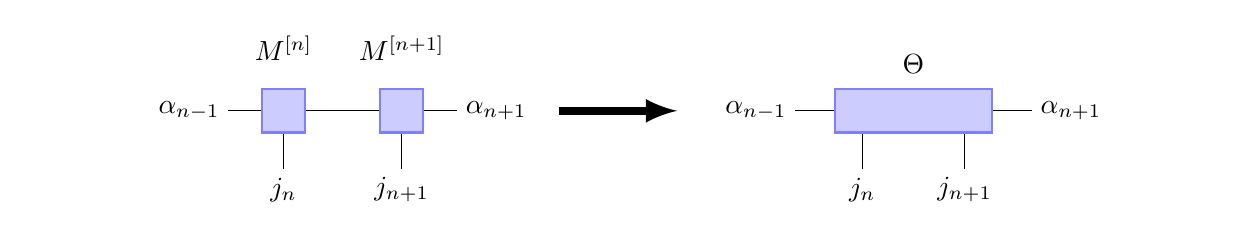
\begin{tikzpicture}[inner sep=1mm]
	\def \imgcenter {5.25};
	\def \imgwidth {15};
	\node[minimum width=\imgwidth cm] (fake) at (\imgcenter ,0) {};


    \node[tensor] (M1) at (1 , 0) {};
    \node[tensor] (M2) at (2.5 , 0) {};
	\node[tensor, minimum width=2cm] (sig) at (9, 0) {};
	
	\node (j1) at (1 ,-1) {$j_n$};
	\node (j2) at (2.5 ,-1) {$j_{n+1}$};
	\node (a1) at (-0.2 ,0) {$\alpha_{n-1}$};
	\node (a2) at (3.7 ,0) {$\alpha_{n+1}$};    
    
	\draw[-] (M1) -- (j1);
	\draw[-] (M1) -- (a1);
	\draw[-] (M1) -- (M2);
	\draw[-] (M2) -- (j2);
	\draw[-] (M2) -- (a2);
	
	
	\node (node1) at (8.35, -1) {$j_n$};
	\node (node2) at (9.65, -1) {$j_{n+1}$};
	\node (as1) at (7 ,0) {$\alpha_{n-1}$};
	\node (as2) at (11 ,0) {$\alpha_{n+1}$};
	
	\draw[-] (node1) -- (node1 |-  sig.south);
	\draw[-] (node2) -- (node2 |-  sig.south);
	\draw[-] (sig) -- (as1);
	\draw[-] (sig) -- (as2);		
	
	\draw[->, line width=1mm] (4.5,0) -- (6,0);
	
	\node (Mlab1) at (1,0.8) {$M^{[n]}$};
	\node (Mlab2) at (2.5,0.8) {$M^{[n+1]}$};
	\node (Siglab) at (9,0.6) {$\Theta$};
	
	
\end{tikzpicture}
	\end{subfigure}\\[.8cm]
	
	\begin{subfigure}{\textwidth}
		\centering
		\caption{\textbf{Solve eigenprobem:}}
		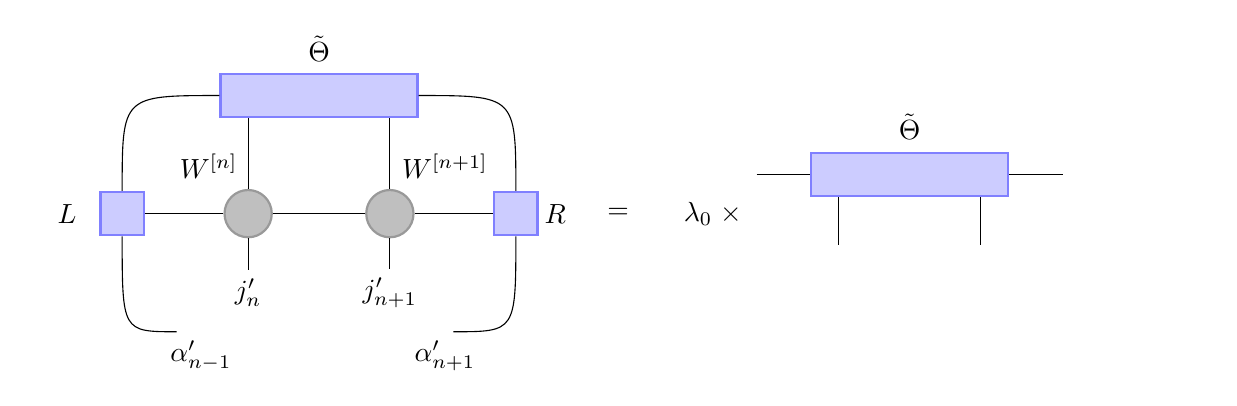
\begin{tikzpicture}[inner sep=1mm]
	\def \imgcenter {5.8};
	\def \imgwidth {15};
	\node[minimum width=\imgwidth cm] (fake) at (\imgcenter ,0) {};	
	
	
	\node[tensor, minimum width=2.5cm] (theta) at (2, 0) {};
	\node[operator] (W1) at (1.1,-1.5) {};
	\node[operator] (W2) at (2.9,-1.5) {};	
	
	\node (dummy1) at (0.3,-3) {};
 	\node (dummy2) at (3.6,-3) {};
	\node[tensor] (L) at (-0.5 , -1.5) {};
	\node[tensor] (R) at (4.5 , -1.5) {};    
    
    \draw[-] (dummy1.west) .. controls (-0.5, -3) .. (L.south);
    \draw[-] (dummy2.east) .. controls (4.5, -3) .. (R.south);
    \draw[-] (theta.west) .. controls (-0.5, 0) .. (L.north);
    \draw[-] (theta.east) .. controls (4.5, 0) .. (R.north);
	
	\draw[-] (L) -- (W1);
	\draw[-] (W1) -- (W2);
	\draw[-] (W2) -- (R);
	\draw[-] (W1) -- (W1 |-  theta.south);
	\draw[-] (W2) -- (W2 |-  theta.south);
	
	\node (j1) at (1.1 , -2.5) {$j_{n}'$};
	\node (j2) at (2.9 , -2.5) {$j_{n+1}'$};
	\draw[-] (W1) -- (j1);
	\draw[-] (W2) -- (j2);
	
	\node (a1) at (0.5 , -3.3) {$\alpha_{n-1}'$};
	\node (a2) at (3.6 , -3.3) {$\alpha_{n+1}'$};
	\node (Llab) at (-1.2 , -1.5) {$L$};
	\node (Rlab) at (5 , -1.5) {$R$};	
	\node (Thetalab) at (2 , 0.6) {$\tilde{\Theta}$};
	\node (W1lab) at (0.6 , -0.9) {$W^{[n]}$};
	\node (W2lab) at (3.6 , -0.9) {$W^{[n+1]}$};
	
	
	\def \offsetx {7.5};
	\def \offsety {-1};
	\node[tensor, minimum width=2.5cm] (theta2) at (2+\offsetx, \offsety) {};
	\node (d1) at (1.1 +\offsetx, -1+ \offsety) {};
	\node (d2) at (2.9 +\offsetx, -1 + \offsety) {};
	\node (d3) at (2+\offsetx - 1.25 - 0.8, 0+\offsety) {};
	\node (d4) at (2+\offsetx + 1.25 + 0.8, 0+\offsety) {};
	
	\draw[-] (d1) -- (d1 |-  theta2.south);
	\draw[-] (d2) -- (d2 |-  theta2.south);
	\draw[-] (d3) -- (theta2);
	\draw[-] (d4) -- (theta2);
	
	\node (Thetalab2) at (2 +\offsetx, 0.6 + \offsety) {$\tilde{\Theta}$};
	
	
	\node (eq) at (5.8 , -1.5) {$=$};
	\node (lambda) at (7 , -1.5) {$\lambda_0 \;  \times$};	
\end{tikzpicture}
	\end{subfigure}\\[.8cm]

	\begin{subfigure}{\textwidth}
		\centering
		\caption{\textbf{Unmerge:}}
		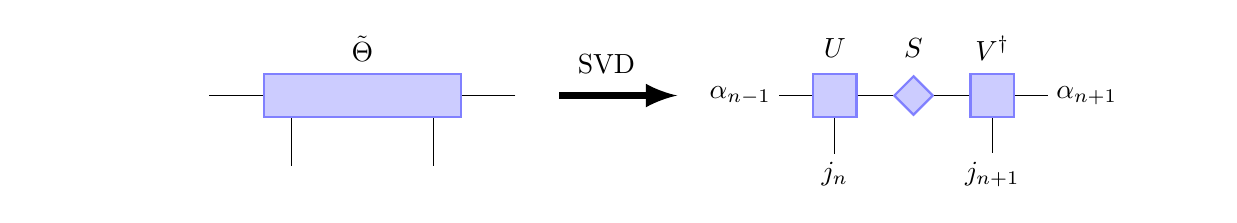
\begin{tikzpicture}[inner sep=1mm]	
	\def \center {2};
	\def \width {2.5};
	\def \offsetx {8};
	\def \xspace {1};
	\def \imgcenter {\offsetx -2.75};
	\def \imgwidth {15};
	\node[minimum width=\imgwidth cm] (fake) at (\imgcenter ,0) {};
	
	
	\node[tensor, minimum width=\width cm] (theta) at (\center, 0) {};
	
	\node (d1) at (\center - \width/2 + 0.35,-1) {};
	\node (d2) at (\center + \width/2 - 0.35,-1) {};
	\node (d3) at (\center - \width/2 - 0.8, 0) {};
	\node (d4) at (\center + \width/2 + 0.8, 0) {};
	
	\draw[-] (d1) -- (d1 |-  theta.south);
	\draw[-] (d2) -- (d2 |-  theta.south);
	\draw[-] (d3) -- (theta);
	\draw[-] (d4) -- (theta);	
	
	\node (thetalab) at (\center , 0 + 0.6) {$\tilde{\Theta}$};
	
	
	\node[tensor] (U) at (\offsetx , 0) {};
	\node[matrix] (S) at (\offsetx + \xspace, 0) {};
    \node[tensor] (V) at (\offsetx + 2*\xspace , 0) {};
	
	
	\node (j1) at (\offsetx ,-1) {$j_n$};
	\node (j2) at (\offsetx + 2*\xspace ,-1) {$j_{n+1}$};
	\node (a1) at (\offsetx -1.2 ,0) {$\alpha_{n-1}$};
	\node (a2) at (\offsetx + 2*\xspace +1.2 ,0) {$\alpha_{n+1}$};    
    
	\node (Ulab) at (\offsetx , 0.6) {$U$};
	\node (Slab) at (\offsetx + \xspace , 0.6) {$S$};
	\node (Vlab) at (\offsetx + 2*\xspace , 0.6) {$V^{\dag}$};    
    
	\draw[-] (U) -- (j1);
	\draw[-] (U) -- (a1);
	\draw[-] (U) -- (S);
	\draw[-] (V) -- (S);
	\draw[-] (V) -- (j2);
	\draw[-] (V) -- (a2);
	
	\draw[->, line width=1mm] (\offsetx-3.5 ,0) -- (\offsetx-2,0);
	\node (SVD) at (\offsetx-2.9 ,0.4) {SVD};
\end{tikzpicture}
	\end{subfigure}\\[.8cm]

	\begin{subfigure}{\textwidth}
		\centering
		\caption{\textbf{Update environments:}}
		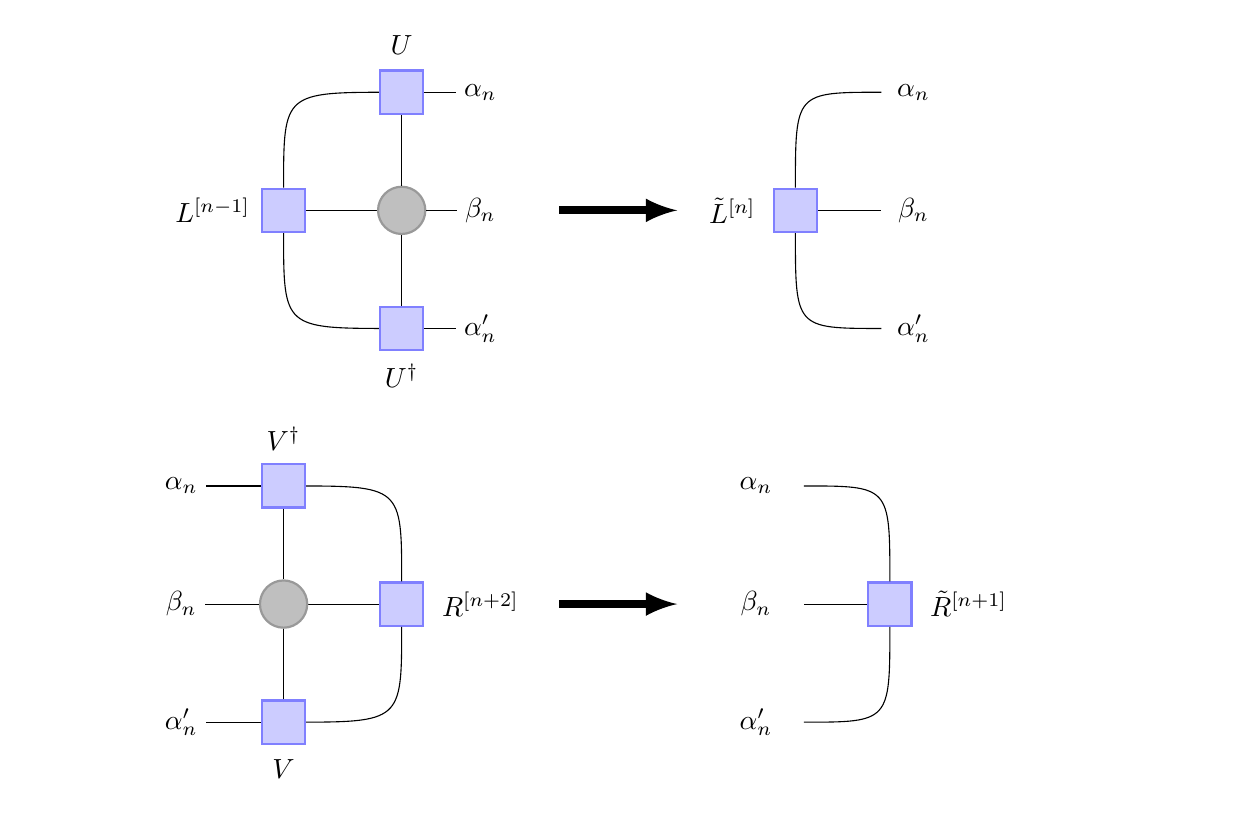
\begin{tikzpicture}[inner sep=1mm]
	\def \offsetx {6};
	\def \offsety {-5};
	\def \imgcenter {\offsetx -2.25};
	\def \imgwidth {15};
	\node[minimum width=\imgwidth cm] (fake) at (\imgcenter ,0) {};
	

	\Left{-0.5}{-1.5}{1.5};
	\node[tensor] (U1) at (1,0) {};	
	\node[tensor] (U2) at (1,-3) {};	
	\node[operator] (W) at (1,-1.5) {};

	\node (a1) at (2,0) {$\alpha_n$};
	\node (a2) at (2,-3) {$\alpha_n '$};
	\node (b) at (2,-1.5) {$\beta_n$};
	
	\draw[-] (U1) -- (W);
	\draw[-] (U2) -- (W);
	\draw[-] (U1) -- (a1);
	\draw[-] (U2) -- (a2);
	\draw[-] (W) -- (b);
	
	\node (L1) at (-1.4,-1.5) {$L^{[n-1]}$};
	\node (U1lab) at (1,0.6) {$U$};
	\node (U2lab) at (1,-3.6) {$U^{\dag}$};
	
	
	\draw[->, line width=1mm] (\offsetx-3 ,-1.5) -- (\offsetx-1.5,-1.5);
	
	
	\Left{\offsetx}{-1.5}{1.2};
	\node (L2) at (\offsetx -0.8,-1.5) {$\tilde{L}^{[n]}$};
	\node (a1) at (\offsetx+1.5,0) {$\alpha_n$};
	\node (a2) at (\offsetx+1.5,-3) {$\alpha_n '$};
	\node (b) at (\offsetx+1.5,-1.5) {$\beta_n$};
	
	%%----------------%%
	
	\Right{1}{-1.5 + \offsety}{1.5};
	\node[tensor] (U1) at (-0.5,0 + \offsety) {};	
	\node[tensor] (U2) at (-0.5,-3 + \offsety) {};	
	\node[operator] (W) at (-0.5,-1.5 + \offsety) {};

	\node (a1) at (-1.8,0 + \offsety) {$\alpha_{n}$};
	\node (a2) at (-1.8,-3 + \offsety) {$\alpha_{n} '$};
	\node (b) at (-1.8,-1.5 + \offsety) {$\beta_{n}$};
	
	\draw[-] (U1) -- (W);
	\draw[-] (U2) -- (W);
	\draw[-] (U1) -- (a1);
	\draw[-] (U2) -- (a2);
	\draw[-] (W) -- (b);
	
	\node (R1) at (2,-1.5 + \offsety) {$R^{[n+2]}$};
	\node (V1lab) at (-0.5,0.6 + \offsety) {$V^{\dag}$};
	\node (V2lab) at (-0.5,-3.6 + \offsety) {$V$};
	
	
	\draw[->, line width=1mm] (\offsetx-3 ,-1.5 + \offsety) -- (\offsetx-1.5,-1.5 + \offsety);
	
	
	\Right{\offsetx + 1.2}{-1.5 + \offsety}{1.2};
	\node (R2) at (\offsetx +2.2,-1.5 + \offsety) {$\tilde{R}^{[n+1]}$};
	\node (a1) at (\offsetx -0.5,0 + \offsety) {$\alpha_{n}$};
	\node (a2) at (\offsetx -0.5,-3 + \offsety) {$\alpha_{n} '$};
	\node (b) at (\offsetx -0.5,-1.5 + \offsety) {$\beta_{n}$};
\end{tikzpicture}
	\end{subfigure}
	
	
	\caption{\textit{A diagrammatic representation of the two-site update sequence for iterative ground state search. In step \textbf{(4)}, which environment is updated is determined by the direction of iteration.}}
	\label{fig:twoSiteUpdate}
\end{figure}

Some comments regarding this sequence are in order: The matrices of the eigenvalue problem have dimensions $( d^2 D^2 \times d^2 D^2)$, which is generally too much for exact diagonalization, however, since only the lowest eigenvalue is of interest, one can use an iterative eigensolver \cite{Lanczos}. Furthermore, if the MPS is not in the proper mixed-canonical form, the eigenvalue problem turns into a generalized eigenvalue problem, which can be numerically quite demanding. Thus, updating the left and right environments in step (4) is necessary, since it leads to great simplifications in step (2). Lastly, one could also consider just a single site when updating, however, this method is very prone to getting stuck \cite{WhiteSingleSite}. By updating two sites at once, one actually optimizes the bond between them. Hence, after updating the two sites, one must only iterate a single site. Optimization is done with regards to the current configuration, whereby it depends on previous updates. To compensate for this, one must sweep through the entire system multiple times, which leads to the following algorithm for iterative ground state search, which follows the structure of the DMRG algorithm:

\begin{algorithm}
\begin{algorithmic}
\caption{Iterative ground state search}
\State Choose $\ket{\psi}$ right-normalized.
\State Calculate tensor $R^{[i]}$ iteratively for $i = N \ldots 1$.
\While{Stopping criteria not met} 
	\For{$n = 1 \ldots N-1$} \Comment{Left sweep}
		\State Perform two-site update on $M^{[n]}$ and $M^{[n+1]}$.
		\State Update $L^{[n]}$ according to eq. \eqref{eq:updateLeft}
	\EndFor
	\For{$n = N-1 \ldots 1$} \Comment{Right sweep}
		\State Perform two-site update on $M^{[n]}$ and $M^{[n+1]}$.
		\State Update $R^{[n]}$ according to eq. \eqref{eq:updateRight}
	\EndFor
\EndWhile
\end{algorithmic}
\end{algorithm}


\subsection{Calculation of Condensate Fraction using DMRG Algorithm}
To illustrate the power of the DMRG algorithm, the following numerical analysis was conducted. As the system of interest is the Bose-Hubbard model described in eq. \eqref{BHhamil}, a suitable benchmark for the algorithm is attempting to calculate the critical point of the phase transition between the Superfluid and Mott-Insulator. The critical point was determined using the DMRG algorithm in \cite{Kuhner2000} by studying the correlations of the system. Here, an alternative approach is presented, which examines the correlation function.\\

According to the Penrose-Onsager criterion, a Bose-Einstein condensate, and by extension the Superfluid state, is present if and only if the largest eigenvalue, $\lambda_1$, of the single-particle density matrix, $\rho^{(1)}$, is macroscopic
\begin{equation}
	f_c = \frac{\lambda_1}{N_{\mathrm{particles}}} > 0 \; ,
	\label{eq:condensateFraction}
\end{equation} 
where $f_c$ is the condensate fraction, and $N_{\mathrm{particles}}$ is the total number of particles \cite{PenroseOnsager}. The condensate fraction can be used to determine which phase dominates the system, as
\begin{align}
	\lim_{N_{\mathrm{particles}} \to \infty} f_{c}^{\mathrm{SF}} &\to 1 \label{eq:SF_lim} \\
	\lim_{N_{\mathrm{particles}} \to \infty} f_{c}^{\mathrm{MI}} &\to 0 \; , \label{eq:MI_lim}
\end{align}
when the filling-fraction, $n = N_{\mathrm{particles}}/N_{\mathrm{sites}}$, is held constant.\\

To calculate the condensate fraction, the ground state of the system was found using the a version of the DMRG algorithm implemented in the ITensor library \cite{ITensor}. Using the computed ground state, $\ket{\psi}$, the entries of the density matrix were calculated
\begin{equation}
	\rho_{i,j} = \bra{\psi} \hat{a}_{i}^{\dag} \hat{a}_{j} \ket{\psi} \; .
\end{equation}
Lastly, the condensate fraction was determined through eq. \eqref{eq:condensateFraction}.
The calculation was performed with varying $U/J$ for various system sizes of unit occupancy. The DMRG algorithm was set to perform 5 sweeps with a maximum bond dimension of 200.
In order to gauge the accuracy of the algorithm, the results for system sizes 4-10 were compared to a similar calculation using exact diagonalisation.
\begin{figure}[h!]
    \centering
    \includegraphics[width=0.7\textwidth]{Figures/CondensateFractionCompare.pdf}
 \caption{\textit{Condensate fraction calculated using the DMRG algorithm with 20 sweeps. The condensate fractions of the smaller systems ($N = 4 \ldots 10$) are compared with result obtained through exact diagonalisation.}}
 \label{fig:CondensateFraction}
\end{figure}
The upper part of figure \ref{fig:CondensateFraction} shows the condensate fraction for various $U/J$ calculated using the DMRG algorithm. In the limit $U/J = 0$, the condensate fraction is unit for the smaller systems, confirming the system is indeed in the Superfluid phase. The condensate fraction never reaches zero, as $U/J$ increases, since this is only achieved in the thermodynamic limit. However, the condensate fraction does decrease with increasing particle number, as would be expected. The lower half of figure \ref{fig:CondensateFraction}  displays the results of the DMRG calculation compared with exact diagonalisation. For small systems the two approaches obtain very similar results.\\
Attempting to use exact diagonalisation for large systems is futile, due to the exponential scaling of the Hilbert space \cite{Vidal2003}. However, this is not an issue using matrix product states, as the formalism only considers a tiny corner of the Hilbert space by following an area law. 
The dashed lines of figure \ref{fig:CondensateFraction} shows the results of the DMRG calculations for up to 50 particles. The condensate fraction behaves as expected in the $U/J \gg 1$ limit, as it tends towards zero for larger particle numbers. Note, in the Superfluid limit the condensate fraction does not quite reach 1. This is due to difficulty of describing long-range correlations when using matrix product states. An extensive explanation of this is given in Section \ref{sec:correlationFunctions}.
This is not an issue for smaller systems, as the correlation length is limited by the system size, due to boundary effects having an influence on a much larger part of the system. \\
Some measures can be taken to minimize errors, when using the DMRG algorithm. Accurately describing long range correlations requires multiple sweeps, as the algorithm has to iteratively approximate an almost constant function with a series of exponentials. Figure \ref{fig:sweepdependence} displays the condensate fraction in the Superfluid limit as a function of number of sweeps. Clearly, performing more sweeps yields a better result.
\begin{figure}[h!]
    \centering
    \includegraphics[width=0.7\textwidth]{Figures/CFsweeps.pdf}
    \caption{\textit{Condensate fraction as a function of number of sweeps of the DMRG algorithm in the Superfluid limit. A max bond dimension of 250 was used.}}
    \label{fig:sweepdependence}
\end{figure}
Furthermore, increasing the maximal bond dimension, $D$, results in a more accurate long-range representation of correlations. Thus, calculating correlation functions for various values of $D$ is a great way of estimating the convergence of the correlations for a given length scale \cite{schollwock}.\\

In \cite{Kuhner2000} the critical point of phase transition between the Superfluid and Mott-Insulator is determined as $\left( \frac{U}{J} \right)_{crit} = 3.37$. The result is achieved through examining the correlations of the systems. While correlations in Mott-Insulators decay exponentially, Superfluids have a decay of correlations following the power-law given in eq. \eqref{sec:correlationFunctions}. As a result, the interface between the two phases, has correlations following a power law determined by the Luttinger liquid parameter. The critical point, which is located at the tip of the Mott-lobes, is computed by determining the point, at which the Luttinger liquid parameter is $K =  \frac{1}{2}$ \cite{Kuhner2000}.\\
Examining figure \ref{fig:CondensateFraction}, one notices a hump on the graph in the vicinity of this critical ratio, but no clear indication of a phase transition is present. In the thermodynamic limit, one would expect the condensate fraction to drop to zero, as the critical ratio is reached (as observed in 2D by \cite{Spielman2008}). However, at 50 particles the condensate fraction is only around $ f_c = 0.5$. One could extrapolate data from computations using different particle numbers in order to determine the location of the critical point. However, this would require computations using larger systems in order to minimize the boundary effects.


\section{Time Evolution of Matrix Product States}
A central component of Optimal Control is time evolution. In order to compute any optimal control sequence, it is crucial to have a fast and accurate time evolution algorithm. However, also the construction of the time evolution operator must be taken into account, as exponentiating a tensor spanning the entire system, such as most Hamiltonians, is no easy task. In fact, since the time evolution operator is constantly altered when optimizing control parameters, the time spent exponentiating the Hamiltonian must be taken into account of the total runtime. Thus, both an efficient time evolution algorithm and an efficient operator exponentiation is needed when performing optimal control.\\
Several algorithms for time evolving matrix product states exist, however, they all origin from the same ideas proposed in \cite{Vidal2003,Vidal2004}. The most widely used of these algorithms is the tDMRG algorithm, which gets its name from its similarity with the ground state search algorithm described in Section \ref{sec:DMRG}. The tDMRG algorithm has been utilized in several instances to simulate the dynamics of one-dimensional systems CITE, and it has even been previously used in conjunction with the CRAB algorithm to perform optimal control of the Superfluid to Mott-Insulator phase transition \cite{FrankBloch,Doria2011}.\\
Although the standard algorithms for time evolution are quite efficient, further improvements can be made to the algorithms when tailoring to the problem at hand. Therefore, a modified version of the tDMRG algorithm is proposed in Section \ref{sec:modTMDRG}, which directly utilizes the properties of the Bose-Hubbard Hamiltonian.


\subsection{The tDMRG Algorithm}
Consider the time evolution of a quantum state
\begin{equation}
	\ket{\psi (t)} = \hat{\mathcal{U}}(t) \ket{\psi (0)} \; ,
\end{equation}
where $\hat{\mathcal{U}}(t) = \e^{ - \im \hat{H} t }$ is the time evolution operator. 
Time evolution of a matrix product states is done in a manner similar to that of ground state search, as the bonds between the tensors are evolved rather than the tensors themselves. Thus, the time evolution operator must be decomposed into two-site tensors. The simplest realisation of this is achieved, when considering a Hamiltonian containing only nearest-neighbour interactions.
Assume the Hamiltonian is a sum of two-site operators of the form $\hat{H} = \sum_{n} \hat{h}^{[n , n+1]}$. One can decompose this into a sum over even and odd bonds
\begin{equation}
	\hat{H} = \hat{H}_{\mathrm{odd}} \; + \; \hat{H}_{\mathrm{even}} = \sum_{n \; \mathrm{odd}} \hat{h}^{[n , n+1]} \; + \; \sum_{n \; \mathrm{even}} \hat{h}^{[n , n+1]} \; .
\end{equation}  
Exponentiating the Hamiltonian is non-trivial due to the non-commutativity of the operators
\begin{equation}
	[ \hat{h}_{\mathrm{odd}}^{[n , n+1]} \; , \; \hat{h}_{\mathrm{even}}^{[n , n+1]} ] \neq 0 \; .
\end{equation}
Considering a small time slice, $\delta t$, the exponentiation can be achieved through the Trotter-Suzuki expansion \cite{Suzuki}. To first order this reads
\begin{equation}
	\e^{- \im \hat{H} \; \Delta t} = \e^{- \im \hat{H}_{\mathrm{odd}} \; \Delta t } \e^{- \im \hat{H}_{\mathrm{even}} \; \Delta t} \; + \; \;  \mathrm{O}(\Delta t^2) \; ,
\end{equation}
where the error is due to the non-commutativity of the bond Hamiltonians. Thus, the time evolution operator can be expressed as the product
\begin{equation}
	\hat{\mathcal{U}}(\Delta t) \approx \left( \prod_{n \; \mathrm{odd}} \hat{\mathcal{U}}^{[n,n+1]} (\Delta t) \right) \left( \prod_{n \; \mathrm{even}} \hat{\mathcal{U}}^{[n,n+1]} (\Delta t) \right) \; ,
\end{equation}
where
\begin{equation}
	\hat{\mathcal{U}}^{[n,n+1]} (\Delta t) = \e^{- \im \hat{h}^{[n , n+1]} \; \Delta t } \; .
\end{equation}
The result is an MPO performing an infinitesimal time step on the odd bonds, and another MPO evolving the even bonds. An illustration of this is shown in Figure \ref{fig:oddevenops}.
\begin{figure}[h!]
	\centering
	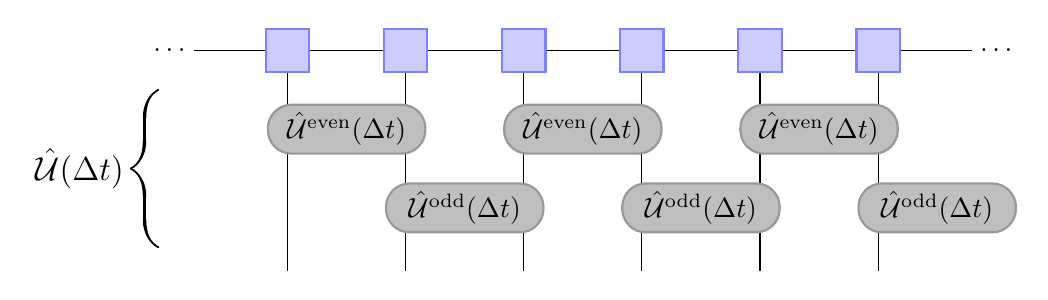
\begin{tikzpicture}[inner sep=1mm]
	\def \reldist {1.5};
	\def \numb {6};
	\def \wid {2}

	\foreach \i in  {1,...,\numb} {
		\node[tensor] (t\i) at (\i * \reldist, 0) {};
		\draw[-] (t\i) -- (\i * \reldist , -2.8);	
	};
	
	\foreach \i in {1,...,5} {
        \pgfmathtruncatemacro{\iplusone}{\i + 1};
        \draw[-] (t\i) -- (t\iplusone);
	};
	
	\foreach \i in {1,3,5} {
        \node[twositeop, minimum width= \wid cm] (op\i) at (\reldist*\i + \wid/2 -0.25,-1) {$\hat{\mathcal{U}}^{\mathrm{even}} (\Delta t)$};
	};
	
	\foreach \i in {2,4,6} {
        \node[twositeop, minimum width= \wid cm] (op\i) at (\reldist*\i + \wid/2 -0.25,-2) {$\hat{\mathcal{U}}^{\mathrm{odd}} (\Delta t)$};
	};	
	
	\node (dot1) at (0,0) {$\dots$};
	\node (dot2) at (\numb * \reldist + \reldist,0) {$\dots$};
	\draw[-] (t1) -- (dot1);
	\draw[-] (t\numb) -- (dot2);
	
	\draw[decoration={calligraphic brace,amplitude=10pt}, decorate, line width=1.25pt, xshift=-4pt, yshift=0pt]
(0, -2.5) -- (0,-0.5) node [black,midway,xshift=-1.0cm] 
{\large $\hat{\mathcal{U}} ( \Delta t)$};
	
\end{tikzpicture}
	\caption{\textit{Approximation of each time step $\delta t$ using a Trotter-Suzuki decomposition, such that the time evolution operator is expressed as a product of unitary two-site operators.}}
	\label{fig:oddevenops}
\end{figure}
The tDMRG algorithm describes the most efficient and accurate way of contracting the tensor network detailed in Figure \ref{fig:oddevenops}. The algorithm gets its name from its similarity with the DMRG algorithm detailed in Section \ref{sec:DMRG}. In fact, the merge and unmerge procedure of the two algorithms is completely identical, whereby they only differ in the steps of applying the operator and proceeding to the next site. The following procedure details a time evolution step of the $n$'th bond \cite{schollwock}.

\subsubsection{Infinitesimal time-step update for tDMRG}
\begin{enumerate}
\item
\textbf{Merge:} Contract tensors $M^{[n]}$ and $M^{[n+1]}$ over the bond $\alpha_{n}$ creating a two-site tensor $\Theta^{j_n , j_{n+1}}$.

\item
\textbf{Apply unitary:} The two-site time evolution operator, $\hat{\mathcal{U}}^{[n, n+1]}$, is applied to $\Theta^{j_n , j_{n+1}}$
\begin{equation}
	\tilde{\Theta}_{\alpha_{n-1} , \alpha_{n+1}}^{j_n , j_{n+1} } = \sum_{j_n ', j_{n+1}'} U^{j_n  j_{n+1} , j_n '  j_{n+1}'} \; \Phi_{\alpha_{n-1} , \alpha_{n+1}}^{j_n ', j_{n+1} ' } \; .
\end{equation}

\item
\textbf{Unmerge:} Reshape $\tilde{\Phi}_{\alpha_{n-1} , \alpha_{n+1}}^{j_n ', j_{n+1} '}$ to a matrix and decompose it through an SVD. Applying $\hat{\mathcal{U}}^{[n, n+1]}$ causes an increase in bond dimension, $D \rightarrow d^2 D$, which must be truncated by keeping only the $D$ largest singular values from the SVD. 

\item
\textbf{Progress:}  Next, the center cite of the MPS must be shifted by two, in order to update the next even (odd) bond. This is achieved by merging tensors $M^{[n+1]}$ and $M^{[n+2]}$ and performing a second SVD, while reshaping the resulting $U$-matrices to left-normalised tensors to retain the canonical form. The product of the second SVD must be truncated as well, however, no loss of information will occur, as the Schmidt rank of the matrix $S$ will be at most $D$ following the first SVD. 
\end{enumerate}
Following the procedure will leave the MPS in position for application ofthe unitary $\hat{\mathcal{U}}^{[n+2 , n+3]}$. The efficiency of the tDMRG algorithm also depends on the sequence in which bonds are evolved. A simple, yet effective way is iterating from left to right when evolving even bonds, while iterating right to left when evolving odd bonds. Thereby, the centered cite of the mixed-canonical form is moved continuously through the MPS, rather than having to be reset when reaching the end of the system.\\

Although the tDMRG algorithm is a very powerful algorithm, an even higher efficiency can be achieved when tailoring the algorithm to the problem. In this case the problem is optimal control of the Superfluid to Mott-Insulator transition. Thus, the Hamiltonian contains both nearest-neighbour and on-site terms. Furthermore, the Hamiltonian is time dependent, and it is continuously modified in the process of searching for optimal control parameters. The following algorithm is a modification of the tDMRG algorithm, which accommodates the requirements of performing optimal control.


\subsection{Modified Time Evolution Algorithm for Optimal Control}
\label{sec:modTMDRG}
In order to efficiently conduct optimal control of a Bose-Hubbard system, a slightly modified version of the tDMRG algorithm was employed. As the Hamiltonian is changing with every time step, one has to account for the time spent exponentiating the operators when considering the runtime of the algorithm. A general operator $\hat{W}$ can be exponentiated through the series expansion
\begin{equation}
	\exp \left( \hat{W} \right) = \sum_{k = 0}^{\infty} \frac{\hat{W}^k}{k!} = \hat{\mathds{1}} + \hat{W} \Bigl(  \hat{\mathds{1}} + \frac{\hat{W}}{2} \Bigl( \hat{\mathds{1}} + \frac{\hat{W}}{3} \Bigl( \ldots
\label{eq:exponentialSeries}
\end{equation}
The number of terms needed in the expansion to accurately describe the exponentiation depends on the operator. Performing the exponentiation through a series expansion is a relatively expensive operator. Therefore, it is crucial to find an easier way of constructing the time evolution operator.
One method is by considering the form of the Bose-Hubbard Hamiltonian. The most natural choice of control parameter is the lattice depth, $V_0$, as it is controllable experimentally. The lattice depth determines both the tunneling matrix element, $J$ (eq. \eqref{eq:BHparamJ}), and the interaction matrix element, $U$ (eq. \eqref{eq:BHparamU}), and has served as control parameter in other studies CITE.   
Unfortunately exponentiating the hopping terms of the Bose-Hubbard Hamiltonian is a relatively costly computation. Therefore, it was concluded that keeping $J$ fixed and using $U$ as the control parameter was the better option. Due to the diagonal form of the number operator, $\hat{n}_i$, the exponentiation of the interaction term can be built directly without the need for the series expansion of eq. \eqref{eq:exponentialSeries}.
However, simply exponentiating the different terms of the Bose-Hubbard Hamiltonian separately is not possible, as the operators do not commute. Therefore, one must expand the time evolution operator into its components through the Suzuki-Trotter expansion. To second order the Suzuki-Trotter expansion reads
\begin{equation}
	\exp\left(  ( \hat{V} + \hat{W}  ) \delta \right) = \exp\left(  \hat{V} \delta /2  \right) \exp\left(  \hat{W} \delta   \right) \exp\left(  \hat{V} \delta /2  \right) + O(\delta^3) \; . \label{eq:SuzukiTrotter}
\end{equation}
Once again, the error is due to the non-commutativity of operators. Thus, the time evolution operator can be divided into a sequence of tensors, where
\begin{align}
	\hat{\mathcal{U}}_{J}^{[i,i+1]} (\Delta t) &= \exp \left( -i J ( \hat{a}_{i}^{\dag} \hat{a}_{i+1} + \hat{a}_{i+1}^{\dag} \hat{a}_{i} ) \Delta t \right) \\
	\hat{\mathcal{U}}_{U}^{[i]} (\Delta t /2) &= \exp \left( -i \frac{U}{2} \hat{n}_i (\hat{n}_i -1) \Delta t /2 \right) \; .
\end{align}
\begin{figure}[h!]
	\centering
	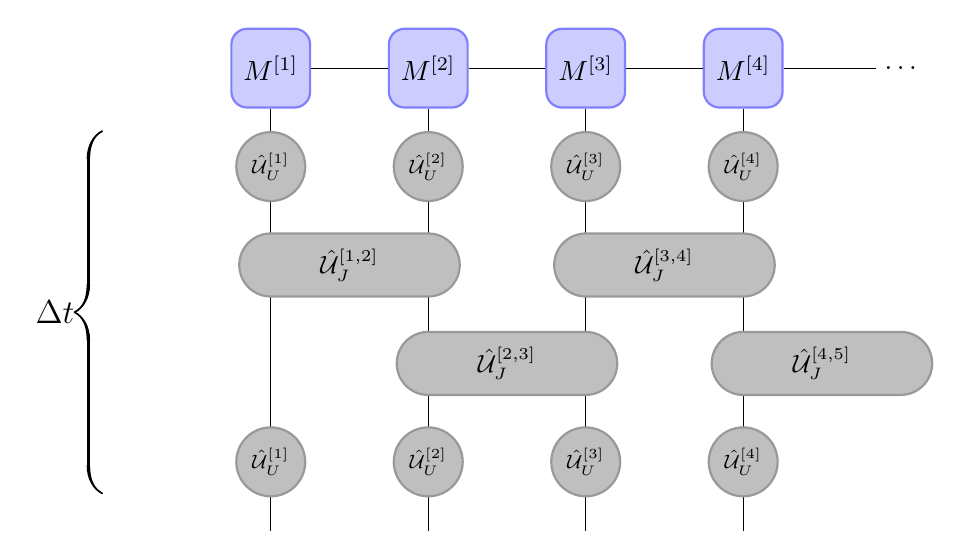
\begin{tikzpicture}[inner sep=1mm]
\def \reldist {2};
\def \numb {4};
\def \wid {2.8};
\def \size {1.0};
\def \hi {0.8};
\def \vert {1.25};
\def \rad {0.4};

	
\foreach \i in  {1,...,\numb} {
	\node[tensor,minimum width= \size cm,minimum height= \size cm, rounded corners = 0.2cm] (A\i)
	at (\i * \reldist, 0) {$M^{[ \i ]}$};
	\draw[-] (A\i) -- (\i * \reldist , -4.7*\vert);	
};

\foreach \i in {1,...,3} {
    \pgfmathtruncatemacro{\iplusone}{\i + 1};
    \draw[-] (A\i) -- (A\iplusone);
};


\foreach \i in  {1,...,\numb} {
	\node[operator,minimum width= \hi cm,minimum height= \hi cm] (op\i)
	at (\i * \reldist, -\vert )
	{\scriptsize $\hat{\mathcal{U}}_{U}^{[ \i ]}$};	
};

\foreach \i in {1,...,\numb} {
	\pgfmathtruncatemacro{\j}{\i + 1};
    \node[twositeop, minimum width= \wid cm,minimum height= \hi cm,rounded corners = \rad cm] (eop\i)
    at (\reldist*\i + \reldist/2, {-2*\vert - Mod(\j,2) *\vert })
    {\small $\hat{\mathcal{U}}_{J}^{[ \i , \j ]} $};
};

\foreach \i in  {1,...,\numb} {
	\node[operator,minimum width= \hi cm,minimum height= \hi cm] (op\i)
	at (\i * \reldist, -4*\vert )
	{\scriptsize $\hat{\mathcal{U}}_{U}^{[ \i ]}$};	
};




\draw[decoration={calligraphic brace,amplitude=10pt}, decorate, line width=1.25pt, xshift=-4pt, yshift=0pt]
(0, -4*\vert -0.4) -- (0,-0.8) node [black,midway,xshift=-0.6cm] 
{\large $\Delta t$};


	\node (dot2) at (\numb * \reldist + 2,0) {$\dots$};

	\draw[-] (A\numb) -- (dot2);
	
	
\end{tikzpicture}
	\caption{\textit{Tensor diagram depicting a single time step of the modified rDMRG algorithm. The time evolution operator has been subjected to a Suzuki-Trotter expansion as detailed in eq. \eqref{eq:SuzukiTrotter}. The tensors of the upper part of the network are contracted with the MPS while sweeping from left to right, whereas the lower part is applied with a right-to-left sweep.}}
	\label{fig:ModifiedTEBD}
\end{figure}
A single time step, $\Delta t$, using the expanded operator is represented diagrammatically in figure \ref{fig:ModifiedTEBD}. At first glance, the tensor network resulting from the Suzuki-Trotter expansion may seem rather extensive, however, it can be contracted in a very efficient manner. The upper part of the network is contracted in a left-to-right sweeping manner, where the position of the center cite, and thereby the normalisation of the MPS, is pushed to the right following each step. Likewise, the lower part of the network is contracted though a right-to-left sweep such that the MPS returns to its original form centered on the first site after applying the final operator. Thereby, the MPS is immediately ready for the subsequent time-propagation.\\
\begin{figure}[h!]
\centering % <-- add this
\begin{subfigure}[b]{0.4\textwidth}
	\caption{}  
  	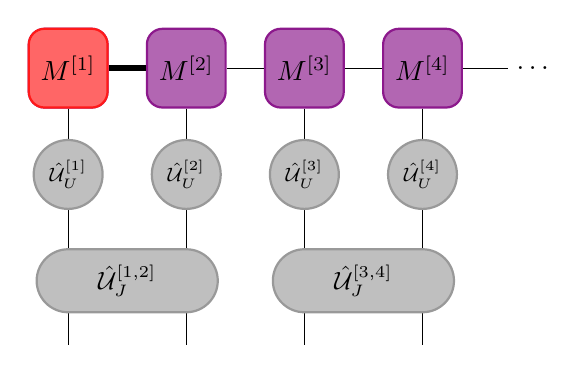
\begin{tikzpicture}[inner sep=1mm]
\def \reldist {1.5};
\def \numb {4};
\def \wid {2.3};
\def \size {1.0};
\def \hi {0.8};
\def \rad {0.4};
\def \vert {1.35};


\foreach \i in  {1,...,\numb} {
	\node[tensorr,minimum width= \size cm,minimum height= \size cm, rounded corners = 0.2cm] (A\i)
	at (\i * \reldist, 0) {$M^{[ \i ]}$};
	\draw[-] (A\i) -- (\i * \reldist , -2.5*\vert);	
};

\foreach \i in {1,...,3} {
    \pgfmathtruncatemacro{\iplusone}{\i + 1};
    \draw[-] (A\i) -- (A\iplusone);
};

\node[tensorc,minimum width= \size cm,minimum height= \size cm, rounded corners = 0.2cm] (C) at (1 * \reldist, 0) {$M^{[1]}$};


\foreach \i in  {1,...,\numb} {
	\draw[-] (A\i) -- (\i * \reldist , -2.6 *\vert);	
};

\draw[-,line width=0.8mm] (A1) -- (A2);

\foreach \i in  {1,...,\numb} {
	\node[operator,minimum width= \hi cm,minimum height= \hi cm] (op\i)
	at (\i * \reldist, -\vert)
	{\scriptsize $\hat{\mathcal{U}}_{U}^{[ \i ]}$};	
};

\foreach \i in {1,3} {
	\pgfmathtruncatemacro{\j}{\i + 1};
    \node[twositeop, minimum width= \wid cm,minimum height= \hi cm,rounded corners = \rad cm] (top\i)
    at (\reldist*\i + \reldist/2, -2*\vert)
    {\small $\hat{\mathcal{U}}_{J}^{[ \i , \j ]} $};
};


\node (dot2) at (\numb * \reldist + 1.4,0) {$\dots$};
\draw[-] (A\numb) -- (dot2);
	
	
\end{tikzpicture}
\end{subfigure}
\hspace{10mm}
\begin{subfigure}[b]{0.4\textwidth}
	\caption{}    
  	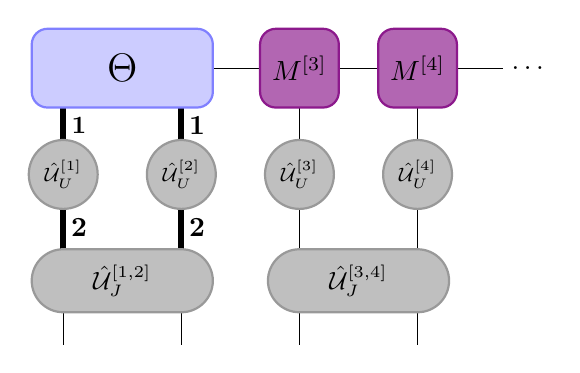
\begin{tikzpicture}[inner sep=1mm]
\def \reldist {1.5};
\def \numb {4};
\def \wid {2.3};
\def \size {1.0};
\def \hi {0.8};
\def \rad {0.4};
\def \vert {1.35};


\foreach \i in  {1,...,\numb} {
	\node[operator] (A\i)
	at (\i * \reldist, 0) {};
	\draw[-] (A\i) -- (\i * \reldist , -2.5*\vert);	
};

\foreach \i in {1,...,3} {
    \pgfmathtruncatemacro{\iplusone}{\i + 1};
    \draw[-] (A\i) -- (A\iplusone);
};


\foreach \i in  {1,...,\numb} {
	\draw[-] (A\i) -- (\i * \reldist , -2.6 *\vert);	
};

\node[operator] (d1) at (1 * \reldist, -\vert) {};
\node[operator] (d2) at (2 * \reldist, -\vert) {};
\node[operator] (dd1) at (1 * \reldist, -2*\vert) {};
\node[operator] (dd2) at (2 * \reldist, -2*\vert) {};


\draw[-,line width=0.8mm] (A1) -- (d1);
\draw[-,line width=0.8mm] (A2) -- (d2);
\draw[-,line width=0.8mm] (dd1) -- (d1);
\draw[-,line width=0.8mm] (dd2) -- (d2);

\foreach \i in  {1,...,\numb} {
	\node[operator,minimum width= \hi cm,minimum height= \hi cm] (op\i)
	at (\i * \reldist, -\vert)
	{\scriptsize $\hat{\mathcal{U}}_{U}^{[ \i ]}$};	
};

\foreach \i in {1,3} {
	\pgfmathtruncatemacro{\j}{\i + 1};
    \node[twositeop, minimum width= \wid cm,minimum height= \hi cm,rounded corners = \rad cm] (top\i)
    at (\reldist*\i + \reldist/2, -2*\vert)
    {\small $\hat{\mathcal{U}}_{J}^{[ \i , \j ]} $};
};


\node (dot2) at (\numb * \reldist + 1.4,0) {$\dots$};
\draw[-] (A\numb) -- (dot2);

\foreach \i in  {3,...,\numb} {
	\node[tensorr,minimum width= \size cm,minimum height= \size cm, rounded corners = 0.2cm] (B\i)
	at (\i * \reldist, 0) {$M^{[ \i ]}$};
};
\node[tensor,minimum width= \wid cm,minimum height= \size cm, rounded corners = 0.2cm] (AA) at (\reldist*1 + \reldist/2, 0) {\Large $\Theta$};



	\node (node1) at (\reldist +0.2, -0.5*\vert -0.05) {\small \textbf{1}};
	\node (node2) at (2*\reldist +0.2, -0.5*\vert -0.05) {\textbf{1}};
	\node (node3) at (\reldist +0.2, -1.5*\vert) {\textbf{2}};
	\node (node4) at (2*\reldist +0.2, -1.5*\vert) {\textbf{2}};	
	
\end{tikzpicture}
\end{subfigure}
\\ % <-- add this
\vspace{5mm}
\begin{subfigure}[b]{0.4\textwidth}
	\caption{}    	
  	\input{Diagrams/TrotterStep4.tex}
\end{subfigure}
\hspace{10mm}
\begin{subfigure}[b]{0.4\textwidth}
	\caption{}  
  	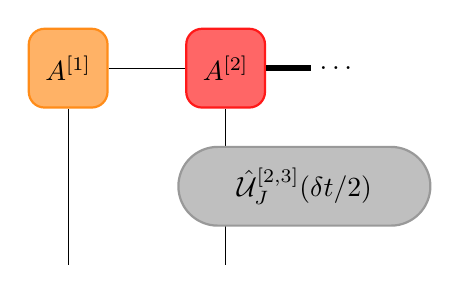
\begin{tikzpicture}[inner sep=1mm]
\def \reldist {2};
\def \numb {2};
\def \wid {3.2};
\def \size {1.0};
\def \rad {0.5};



\node[tensorl,minimum width= \size cm,minimum height= \size cm, rounded corners = 0.2cm] (A1) at (1 * \reldist, 0) {$A^{[1]}$};

\node[tensorc,minimum width= \size cm,minimum height= \size cm, rounded corners = 0.2cm] (A2) at (2 * \reldist, 0) {$A^{[2]}$};


\foreach \i in  {1,...,\numb} {
	\draw[-] (A\i) -- (\i * \reldist , -2.5);	
};

\draw[-] (A1) -- (A2);    

\node[twositeop, minimum width= \wid cm,minimum height= \size cm,rounded corners = \rad cm] (fop2)
    at (\reldist*2 + \reldist/2, -1.5 )
    {$\hat{\mathcal{U}}_{J}^{[2,3]}(\delta t /2)$};


\node (dot2) at (\numb * \reldist + 1.4,0) {$\dots$};
\draw[-,line width=0.8mm] (A\numb) -- (dot2);
	
	
\end{tikzpicture}
\end{subfigure}
\caption{\textit{Sequence of contractions for modified tDMRG algorithm during left to right sweep. Step \textbf{(i)}: MPS is centered on site 1. Tensors $M^{[1]}$ and $M^{[2]}$ are contracted. Step \textbf{(ii)}: Two-site tensor, $\Theta$, is contracted with operators in numbered sequence. The propagated two-site tensor is split using an SVD in step \textbf{(iii)}, followed by a contraction to the right. Lastly, in step \textbf{(iv)}, the two-site tensor of $M^{[2]}$ and $M^{[3]}$ is split using another SVD, whereby the center (and thereby the normalisation) is pushed to site 3.}}
\label{fig:TEBDContraction}
\end{figure}
The sequence of contractions of the left-to-right sweep is shown in figure \ref{fig:TEBDContraction}. The MPS is initially centered on the first tensor, while its remaining tensors are all right-normalised. By contracting the bonds marked with a bold line, the operators are efficiently applied to the MPS. In step (iii) the two-site tensor, $\Theta$, is split using an SVD, where the bond dimension of the tensors is truncated. This is crucial in order to maintain a reduced dimensionality, which would otherwise result in a significant increase in contraction time. In the final step (iv), the central cite of the MPS is moved to the start of the next two-site operator through another site merge and subsequent SVD. This step is exactly as in the original tDMRG algorithm. Thereby the normalisation of the MPS is "pushed" to the right and contained in a single site, which makes it easy to deal with in the end of the time evolution step.\\
As the center reaches the end of the MPS, the direction of the sweep is reversed. The right-to-left sweep is very similar to the sequence described above. The main difference is in the order of contractions, as the $\hat{\mathcal{U}}_{J}^{[i,i+1]} (\Delta t)$-operator is applied before the $\hat{\mathcal{U}}_{U}^{[i]} (\Delta t /2)$-operator. As the sweep, and thereby the central cite, reaches the first site of the MPS, the central site is divided by its norm. Thereby the MPS is normalised and in the same configuration as before the time step. Thus, further propagations can be performed readily.\\ 
Additional precision is achieved when evaluating the potential at the beginning and end points of the time interval CITE DANIEL STECK. Thus, the left-to-right sweep applies the operator $\hat{\mathcal{U}}_{U(t)}^{[i]} (\Delta t /2)$, while the right-to-left sweep applies $\hat{\mathcal{U}}_{U(t + \Delta t)}^{[i]} (\Delta t /2)$.


\subsubsection{Gradient of Suzuki-Trotter propagator}
In section \ref{sec:GRAPE} the derivative of the cost function with regards to the control was derived for a general propagator. However, expanding the propagator using the Suzuki-Trotter expansion while having a diagonal control Hamiltonian causes all higher order contributions of the gradient to drop out. Instead, the precision of the gradient is solely determined by the order of the expansion.\\
Consider the gradient entries for the cost function
\begin{equation}
	\frac{\partial J}{\partial u_n (t_j)} = - \Re \Braket{\chi (t_j) | i \frac{ \partial \hat{\mathcal{U}}_{j}}{\partial u_n (t_j)} | \psi (t_{j-1})} \; ,
\end{equation}
where the derivative of a general propagator with respect to the control is given by
\begin{equation}
	\frac{\partial \hat{\mathcal{U}}_{j}}{\partial u_n (t_j)} = e^{-i \hat{H} (u_n (t_j)) \Delta t}  \sum_{k = 0}^{\infty }  \frac{i^k \Delta t^{k+1}}{(k+1)!} \left[ \hat{H} (u_n (t_j)) , \frac{\partial \hat{H} (u_n (t_j))}{\partial u_n (t_j)}  \right]_k \;.
\end{equation}
The algorithm in this instance employs a Suzuki-Trotter expansion of the propagator while considering the control at both start and end of the step. For cleaner notation the Hamiltonian, which in this case is the Bose-Hubbard Hamiltonian of eq. \eqref{BHhamil}, will be parametrized as $\hat{H}(U(t_j)) \equiv \hat{H}_J + U(t_j) \hat{H}_U$. Note, that the control in this instance is the interaction strength, $u_n (t_j) \equiv U (t_j)$. Thus, the full propagator reads
\begin{equation}
	\hat{\mathcal{U}}_{j}^{\mathrm{ST}} = \exp \left( -i U(t_j) \hat{H}_U \Delta t /2 \right) \exp \left( -i \hat{H}_J \Delta t \right) \exp \left( -i  U(t_{j-1}) \hat{H}_U  \Delta t /2 \right)  \equiv \hat{\mathcal{U}}_{j}^{U} \hat{\mathcal{U}}_{j}^{J} \hat{\mathcal{U}}_{j-1}^{U} \; .
\end{equation}
Since the control at times $t_j$ and $t_{j-1}$ both contribute to $\hat{\mathcal{U}}_{j}^{\mathrm{ST}}$, the elements of the cost gradient are
\begin{equation}
	\frac{\partial J}{\partial U (t_j)} = - \Re \Braket{\chi (t_j) | i  \frac{\partial \hat{\mathcal{U}}_{j}^{\mathrm{ST}}}{\partial U (t_j)} | \psi (t_{j-1})} - \Re \Braket{\chi (t_{j+1}) | i \frac{ \partial \hat{\mathcal{U}}_{j+1}^{\mathrm{ST}}}{\partial U (t_j)} | \psi (t_{j})} \; . \label{eq:STcostderiv}
\end{equation}
Further examining the derivative of the first propagator reveals
\begin{align}
	\frac{\partial \hat{\mathcal{U}}_{j}^{\mathrm{ST}}}{\partial U (t_j)} &=  \frac{\partial \hat{\mathcal{U}}_{j}^{U}}{\partial U (t_j)} \hat{\mathcal{U}}_{j}^{J} \hat{\mathcal{U}}_{j-1}^{U} \nonumber \\
	&=  \exp \left( -i U (t_j) \hat{H}_U  \Delta t /2 \right)  \sum_{k = 0}^{\infty }  \frac{i^k \Delta t^{k+1}}{(k+1)!} \left[ U (t_j) \hat{H}_U  ,  \hat{H}_U \right]_k \hat{\mathcal{U}}_{j}^{J} \hat{\mathcal{U}}_{j-1}^{U} \nonumber \\
	&= \left(  \hat{H}_U \Delta t /2 \right) \exp \left( -i U(t_j) \hat{H}_U  \Delta t /2 \right)   \hat{\mathcal{U}}_{j}^{J} \hat{\mathcal{U}}_{j-1}^{U} \nonumber \\
	&= \left(  \hat{H}_U \Delta t /2 \right) \hat{\mathcal{U}}_{j}^{\mathrm{ST}} \; . \label{eq:STpropderiv1}
\end{align}
Since $\hat{H}_U$ is diagonal, the following relation apply for the recursive commutator 
\begin{equation}
	\left[ U (t_j) \hat{H}_U  ,  \hat{H}_U \right]_k =  
	\begin{cases}
    	\hat{H}_U, & \text{if $k = 0$}.\\
    	0, & \text{otherwise}.
  	\end{cases} \; ,
\end{equation}  
which causes all higher-order contributions to the derivative of the propagator to drop out.\\
Likewise, the derivative of the second propagator is
\begin{equation}
	\frac{\partial \hat{\mathcal{U}}_{j+1}^{\mathrm{ST}}}{\partial u_n (j)} =  \hat{\mathcal{U}}_{j+1}^{\mathrm{ST}} \left(  \hat{H}_U \Delta t /2 \right) \; . \label{eq:STpropderiv2}
\end{equation}
Inserting the derivatives of eq. \eqref{eq:STpropderiv1} and \eqref{eq:STpropderiv2} into the derivative of the cost (eq. \eqref{eq:STcostderiv}) yields
\begin{align}
	\frac{\partial J}{\partial U (t_j)} &= - \Re \Braket{\chi (t_j) | i  \left(  \hat{H}_U \Delta t /2 \right) \hat{\mathcal{U}}_{j}^{\mathrm{ST}} | \psi (t_{j-1})} - \Re \Braket{\chi (t_{j+1}) | i \hat{\mathcal{U}}_{j+1}^{\mathrm{ST}} \left(  \hat{H}_U \Delta t /2 \right) | \psi (t_{j})} \nonumber \\
	&= - \Re \Braket{\chi (t_j) | i    \hat{H}_U \Delta t /2  | \psi (t_{j})} - \Re \Braket{\chi (t_{j}) | i    \hat{H}_U \Delta t /2   | \psi (t_{j})} \nonumber \\
	&= - \Re \Braket{\chi (t_j) | i \hat{H}_U \Delta t | \psi (t_{j})} \; . \label{eq:STcostgrad}
\end{align}  
Thus, the combination of the Suzuki-Trotter expansion and a diagonal control Hamiltonian eliminates all higher order contributions to the gradient. Thereby, the gradient of the cost is exact up to the order of the expansion.
\begin{figure}[h!]
    \centering
    \includegraphics[width=0.8\textwidth]{Figures/CompareGradientsGRAPE.pdf}
    \caption{\textit{\textbf{(a)}: Numerical gradient along with gradient calculated via eq. \eqref{eq:STcostgrad}. \textbf{(b)}: Difference between the two gradients. \textbf{(c)}: Absolute relative difference between the two gradients.}}
    \label{fig:CompareGradientsGRAPE}
\end{figure}
A comparison between a numerically calculated gradient and the analytically derived gradient of eq. \eqref{eq:STcostgrad} can be seen in Figure \ref{fig:CompareGradientsGRAPE}. The difference between the two gradients is largest at the beginning of the sequence, due to the accumulated error from the time evolution, since $\ket{\chi (0)}$ is derived from two time evolutions over the entire duration.


\subsubsection{Time complexity of time-evolution algorithms}
The Suzuki-Trotter expansion \eqref{eq:SuzukiTrotter} does not determine the ordering of the operators. Thus, an alternative algorithm exists, where the half-step is taken through the $\hat{\mathcal{U}}_{J}^{[i,i+1]}$ operator. However, applying the two-site operators are in general more time consuming than applying two single-site operator.
\begin{figure}[h!]
    \centering
    \includegraphics[width=0.7\textwidth]{Figures/CompareRuntime.pdf}
    \caption{\textit{Runtime of performing 100 time steps with various algorithms in Bose Hubbard system with unit occupancy. Solid lines are systems with a local Fock space of dimension $N$, while dashed lines are systems with a constant Fock space dimension of 5.}}
    \label{fig:CompareRuntime}
\end{figure}
A comparison between the run-times of various time-evolution algorithms in shown in Figure \ref{fig:CompareRuntime}. The two tDMRG algorithms are the one described above using a half-step of $\hat{\mathcal{U}}_{J}$ and $\hat{\mathcal{U}}_{U}$ respectively. The MPO-based algorithm builds the propagator using ITensor library methods following \cite{Pollmann2015}, and the resulting MPO is applied to the MPS according to eq. \eqref{eq:optBracketsMPO}. This method has an error of order $O(\Delta t ^2)$, which is less accurate than the second-order Trotter expansion.
In Section \ref{sec:MPO} the cost of applying an MPO to an MPS was given by $\mathrm{O}(N d^2 D_W ^2 D^2)$. Considering the single-site tensors of the tDMRG algorithms, $D_W$ is zero. Since $d = N$ for the solid lines in Figure \ref{fig:CompareRuntime}, the runtime of the algorithm will have a cubic scaling with the system size. However, a much better scaling can be achieved by truncating the local Hilbert space, such that $d$ is kept constant resulting in a runtime scaling linearly with the system size.
Consider the case of the Bose Hubbard model, eq. \eqref{BHhamil}. The interaction term scales quadratically with the number of particles at a given site, which causes a huge energy penalty even in low end of the tight binding limit. Thus, for large systems with unit occupation, neglecting contributions from states with a majority of the particles at a single site is a reasonable approximation.
Therefore, the modified tDMRG algorithm can be applied to very large systems at a low cost, if the dimension of the physical index of the MPS is restricted to a reasonable fraction of the number of particles.   
\chapter{Results}


summarize the methods used \\
explain how chapter is ordered/which things are examined



\section{Characterization of Methods on Small System}

\subsection{Seed selection}
The success of an optimization process is often dependent on the quality of the initial starting point or seed. Poor seeding strategies can lead to failure in finding optimal solutions when conducting local searches in complex optimization landscapes \cite{Sorensen2016}. This has been demonstrated to occur in constrained quantum control problems \cite{Zhdanov2015}, which is exactly the type of problem examined in this thesis. Hence, the type of seed used for the optimization must be chosen carefully.\\ 
In CITEZAC different adiabatic lattice ramps from the superfluid to Mott-insulator phase were examined. The study concluded that ramping the lattice slowly around the point of the phase transition results in an improved final fidelity. This is very similar to an avoided crossing in a two-level system, $\{ \ket{1} , \ket{2} \}$, due to an external perturbation. In this scenario $\ket{1}$ is the ground state in one asymptotic limit of the external parameter, while $\ket{2}$ is the ground state in the other limit. A transfer $\ket{1} \to \ket{2}$ while remaining in the ground state can be achieved by adiabatically sweeping over the external parameter, whereas a rapid change in this external parameter will result in the final state being excited.\\
Thus, a ramp sequence was proposed in CITEZAC, which has an initial sigmoid shape followed by a slow increase in the lattice depth around the phase transition point. Following this, the lattice follows an exponential ramp to its final depth. Examining other attempts of optimizing the ramp sequence of the Bose-Hubbard model \cite{Doria2011,FrankBloch} shows similar traits in their results. Thus, choosing seeds with a slow ramp across the point of the phase transition followed by a rapid increase in lattice depth should yield good optimization results.


%----------------------------------------------------------------------------------------
%	BIBLIOGRAPHY
%----------------------------------------------------------------------------------------

\printbibliography[heading=bibintoc]

%----------------------------------------------------------------------------------------
%	THESIS CONTENT - APPENDICES
%----------------------------------------------------------------------------------------

\appendix % Cue to tell LaTeX that the following "chapters" are Appendices

\chapter{Example: Quantum Speed Limit in Landau-Zener Model} \label{chap:LZexample}
To illustrate concepts from quantum optimal control theory, a state transfer within the Landau-Zener model is optimized using the GRAPE algorithm.\\
The Landau-Zener model is a two-level system with the general Hamiltonian
\begin{align}
	\hat{H}_{\mathrm{LZ}} = \begin{pmatrix}
    	 \Delta (t) & \Omega_R    \\
         \Omega_R & -\Delta (t) 		
    \end{pmatrix}  = \Omega_R \hat{\sigma}_x + \Delta (t) \hat{\sigma}_z \; , \label{eq:LZhamiltonian}
\end{align}
where $\Omega_R$ is the positive Rabi-frequency, $\Delta (t)$ is the detuning, and $\hat{\sigma}_i$ are the Pauli spin matrices. In such a system the detuning will be the control parameter, as it is easily to manipulate in an experimental setup. An advantage of the Landau-Zener system is that an analytical solution to the control problem exists for arbitrary initial and final states. Two level systems can be illustrated on the Bloch sphere, which depicts the population of the two levels along with the relative phases. Consider the transfer between the initial state
\begin{equation}
\lvert \psi_0 \rangle = \cos{\left(\frac{\theta_0}{2}\right)} \lvert 0 \rangle + e^{i\phi_0}\sin{\left(\frac{\theta_0}{2}\right)}\lvert 1 \rangle 
\end{equation}
and final state
\begin{equation}
\lvert \psi_T \rangle = \cos{\left(\frac{\theta_T}{2}\right)} \lvert 0 \rangle + e^{i\phi_T}\sin{\left(\frac{\theta_T}{2}\right)}\lvert 1 \rangle \; ,
\end{equation}
which are both expressed in terms of the angles of the Bloch sphere.
In CITE the quantum speed limit of such a state transfer was derived to be 
\begin{equation}
	T_{\mathrm{QSL}} = \lvert \frac{\theta_T - \theta_0}{2 \Omega_R} \rvert \; . 
\end{equation}
Consider the case of $\ket{\psi_0} = \ket{0}$ and $\ket{\psi_T} = \ket{1}$, whereby the quantum speed limit is $T_{\mathrm{QSL}} = \frac{\pi}{2 \Omega_R}$. 

\subsubsection{Optimal control using GRAPE} 
In this example $\Omega_R = 1$ for simplicity. Examining the Hamiltonian of eq. \eqref{eq:LZhamiltonian}, it is clear that the state transfer $\ket{0} \to \ket{1}$ can be achieved efficiently by letting $u(t) \equiv \Delta (t) = 0$ for the entire duration. To avoid this the control is subjected to the boundary conditions $u(0) = 0$ and $u(T) = 2 T$.\\
\begin{figure}[h!]
\centering % <-- add this
\begin{subfigure}[b]{0.48\textwidth}
	\caption{}  
  	\includegraphics[width=\textwidth]{Figures/LZcontrol1.pdf}
\end{subfigure}
\hspace{3mm}
\begin{subfigure}[b]{0.48\textwidth}
	\caption{}    
  	\includegraphics[width=\textwidth]{Figures/LZpath1.pdf}
\end{subfigure}

\caption{\textit{Optimal control of LZ-system using GRAPE for $T_1 = \pi / 2$. \textbf{(a)}: Initial and optimized control sequence. \textbf{(b)}: Path traced out on the Bloch sphere by the quantum state, as it is evolved according to the control.}}
\label{fig:LZopt1}
\end{figure}
Figure \ref{fig:LZopt1} displays the results of optimizing the state transfer using the GRAPE algorithm for duration $T_1 = \pi / 2$. The algorithm takes an initial linear seed, which clearly does not reach the target state. Clearly, the optimized control achieves perfect transfer. This is as expected, as the quantum speed limit for the transfer is $T_{\mathrm{QSL}} = T_1 = \pi / 2$, whereby a solution should exist for this duration. However, any duration shorter should not be sufficient to reach the target state.\\ 
\begin{figure}[h!]
\centering % <-- add this
\begin{subfigure}[b]{0.48\textwidth}
	\caption{}  
  	\includegraphics[width=\textwidth]{Figures/LZcontrol2.pdf}
\end{subfigure}
\hspace{3mm}
\begin{subfigure}[b]{0.48\textwidth}
	\caption{}    
  	\includegraphics[width=\textwidth]{Figures/LZpath2.pdf}
\end{subfigure}

\caption{\textit{Optimal control of LZ-system using GRAPE for $T_2 = 2$. \textbf{(a)}: Initial and optimized control sequence. \textbf{(b)}: Path traced out on the Bloch sphere by the quantum state, as it is evolved according to the control.}}
\label{fig:LZopt2}
\end{figure}
Next, consider figure \ref{fig:LZopt2}, which shows the optimization results for duration $T_2 =  2$. As this duration is larger than the quantum speed limit, a solution exist for $T_2$. However, the path of the state on the Bloch sphere is much less direct than for the previous case. This is a consequence of how the optimal control is formulated, as one is searching for a control resulting in $\ket{\psi (T)} = \ket{\psi _{\mathrm{Target}}}$. Thus, the path of state has no impact on the cost.\\ For large duration solutions to the control problem generally become more abundant CITE. Figures \ref{fig:LZopt1} and \ref{fig:LZopt2} illustrate this point, as many different paths from $\ket{\psi _0} \to \ket{\psi _{\mathrm{Target}}}$ are possible for large durations, whereas only few possible solutions are available at durations close to the quantum speed limit.
\chapter{Diagrammatic Representation of Matrix Product States} \label{chap:diagrams}

Due to the many indices, equations describing contractions of matrix product states are often quite hard to read. Therefore, the equations are often represented graphically through diagrams. Many variations of diagrams exists, however, they all follow some general rules:
\begin{itemize}
\item
Tensors are represented by nodes.
\item
Indices are represented by lines. Horisontal lines are \textit{bond indices}, while vertical lines are \textit{physical indices}.
\item
Tensors connected by a line are contracted over said bond.
\end{itemize}
Through these basic rules, most equations involving matrix product states can be expressed through diagrams. In this instance, the color or shape of a node provides information regarding the properties of the tensor. Therefore, the tensors shown in this thesis follow these guidelines:
\begin{itemize}
\item
Tensors part of an MPS are square-like. The color of the tensor denotes its normalisation, as shown in figure \ref{fig:MPStensors}. These different types of normalisation are the essence of MPS canonical forms (see Section \ref{sec:canonical}).
\item
Tensors part of MPO's are grey and circular/elliptical depending on the number of sites they span over. These tensors have two vertical legs compared two the one leg of the MPS tensors.
\item
Matrices (tensors without any physical index) are depicted as a diamond. These often occur after a singular value decomposition. 
\end{itemize} 


\begin{figure}[h!]
\centering % <-- add this
\begin{subfigure}[t]{0.2\textwidth}
	\caption{}  	
  	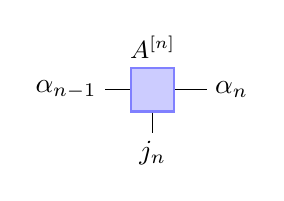
\begin{tikzpicture}[inner sep=1mm]
	\node[tensor, label={\small $A^{[n]}$}] (tensor1) at (0, 0) {};
	\node (index1) at (0, -0.8) {$j_n$};
	\node (index2) at (1.0, 0) {$\alpha_{n}$};
	\node (index3) at (-1.1, 0) {$\alpha_{n-1}$};
	
	\draw[-] (tensor1) -- (index1);
	\draw[-] (tensor1) -- (index2);
	\draw[-] (tensor1) -- (index3);
\end{tikzpicture}
\end{subfigure}
\hspace{5mm}
\begin{subfigure}[t]{0.2\textwidth}    
	\caption{}  	
  	\input{Diagrams/singleLTensor.tex}
\end{subfigure}
\hspace{5mm}
\begin{subfigure}[t]{0.2\textwidth}    
	\caption{}  	
  	\input{Diagrams/singleRTensor.tex}
\end{subfigure}
\hspace{5mm}
\begin{subfigure}[t]{0.2\textwidth}    
	\caption{}  	
  	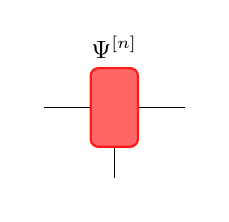
\begin{tikzpicture}[inner sep=1mm]
	\node[tensorc, label={\small $\Psi^{[n]}$}] (tensor1) at (0, 0) {};
	\node (index1) at (0, -1) {};
	\node (index2) at (1, 0) {};
	\node (index3) at (-1, 0) {};
	
	\draw[-] (tensor1) -- (index1);
	\draw[-] (tensor1) -- (index2);
	\draw[-] (tensor1) -- (index3);
\end{tikzpicture}
\end{subfigure}
\caption{\textit{The four different types of MPS tensors used in diagrams. \textbf{(i)} General tensor of un-specified normalisation. The indices corresponding to the tensor are labeled. The remaining tensors are: Left-normalised \textbf{(ii)}, right-normalised \textbf{(iii)}, central cite \textbf{(iv)}. }}
\label{fig:MPStensors}
\end{figure}
	

\chapter{Example: Building an MPO from a Hamiltonian}
\label{chap:buildMPO}
Consider the Bose-Hubbard Hamiltonian , which consists of both nearest-neighbour tunneling terms and on-site interactions terms
\begin{equation}
	\hat{H} = - J \sum_{\langle i,j \rangle} \hat{a}_{i}^{\dag} \hat{a}_{j} + \frac{U}{2} \sum_{i} \hat{n}_i \left( \hat{n}_i -1 \right) \; .
	\label{eq:BHhamil}
\end{equation}
The Hamiltonian can be expressed as a sum of strings of operators - most of these being identities just like in equation \ref{eq:localOperator}. Moving through such a string from the right, one will at some point encounter one of 3 non-trivial operators. This can be summarized as 4 different possible states of the string of operators on a given bond:
\begin{enumerate}
	\item
	Only identities to the right of the bond.
	\item
	An $\hat{a}^{\dag}$ operator just to the right of the bond.
	\item
	An $\hat{a}$ operator just to the right of the bond.
	\item
	A completed tunneling \textit{or} the interaction term, $\frac{U}{2} \hat{n} \left( \hat{n} -1 \right)$, somewhere to the right.
\end{enumerate}
When moving through the string of operators from the right, only certain transitions between these state are possible. For instance $\boldsymbol{1 \rightarrow 1}$, where one starts in state 1, and the next operator is an identity. Likewise, $\boldsymbol{1 \rightarrow 2,3,4}$ are all possible, since these transitions represent the next operator being non-trivial. Next, $\boldsymbol{2 \rightarrow 4}$ completes the hopping $-J \hat{a}^{\dag} \hat{a}$ - a similar transition exists for the other hopping term $\boldsymbol{3 \rightarrow 4}$. Finally, the transition $\boldsymbol{4 \rightarrow 4}$ is needed to continue iterating through the operator chain after having passed the non-trivial operators. This can be encoded in the operator-valued matrix
\begin{equation}
 W^{[i]} \: = \: \begin{pmatrix}
\hat{I} & 0 & 0 & 0  \\
\hat{a}^{\dag} & 0 & 0 & 0  \\
\hat{a} & 0 & 0 & 0 \\
\frac{U}{2} \hat{n} \left( \hat{n} -1 \right) & -J \hat{a} & -J \hat{a}^{\dag} &  \hat{I}
\end{pmatrix} \; ,
\label{eq:MPOmatrix}
\end{equation}
which contains all the allowed transitions between the five state \cite{schollwock}. When one starts moving through the operator chain from the right side, one obviously begins in state 1 and ends in state 4. This can be encoded in the two vectors
\begin{equation*}
 \vec{v}_{left} = (0 , 0 , 0  , 1) \quad , \quad \vec{v}_{right} = (1  , 0 ,0 , 0)^T \; .
\end{equation*}
Thus, the Bose-Hubbard Hamiltonian can be written as an MPO 
\begin{equation}
	\hat{H} = \sum_{\boldsymbol{j}, \boldsymbol{j'}} \vec{v}_{left} \; W^{[1] j_1 , j_1 '} W^{[2] j_2 , j_2 '} \ldots W^{[N] j_N , j_N '} \; \vec{v}_{right} \; \ket{\boldsymbol{j}} \bra{\boldsymbol{j'}} \; .
	\label{eq:MPOhamiltonian}
\end{equation}
Often, the two closing vectors are implicitly multiplied unto the outer matrices for a cleaner notation. Observe how all of this was done without having to do a single numerical computation. The resulting MPO can now readily be applied to an MPS.


%----------------------------------------------------------------------------------------

\end{document}  
